% ===========================================================================
% MAIN FILE — APV-AD Paper
% Amidou Maiga — Erciyes University
% Compile on Overleaf: pdflatex → bibtex → pdflatex → pdflatex
% ===========================================================================

\documentclass[12pt, a4paper]{article}

% ── Encoding & language ─────────────────────────────────────────────────────
\usepackage[utf8]{inputenc}
\usepackage[T1]{fontenc}
\usepackage[english]{babel}

% ── Mathematics ─────────────────────────────────────────────────────────────
\usepackage{amsmath, amssymb}

% ── Graphics & tables ───────────────────────────────────────────────────────
\usepackage{graphicx}
\usepackage{booktabs}
\usepackage{tabularx}
\usepackage{multirow}
\usepackage{multicol}
\usepackage{caption}
\usepackage{subcaption}
\usepackage[table]{xcolor}
\usepackage{float}
\usepackage{makecell}

% ── Layout ──────────────────────────────────────────────────────────────────
\usepackage{geometry}
\geometry{a4paper, margin=2.5cm}
\usepackage{setspace}
\onehalfspacing
\usepackage{parskip}
\setlength{\parindent}{1cm}

% ── Lists ───────────────────────────────────────────────────────────────────
\usepackage{enumitem}

% ── Units ───────────────────────────────────────────────────────────────────
\usepackage{siunitx}
\sisetup{separate-uncertainty=true}
\DeclareSIUnit{\MWh}{MWh}
\DeclareSIUnit{\kWh}{kWh}
\DeclareSIUnit{\Wp}{W_{p}}

% ── Algorithm ───────────────────────────────────────────────────────────────
\usepackage[ruled, vlined, linesnumbered]{algorithm2e}

% ── Hyperlinks ──────────────────────────────────────────────────────────────
\usepackage{hyperref}
\hypersetup{
    colorlinks = true,
    linkcolor  = blue,
    citecolor  = blue,
    urlcolor   = blue,
    pdftitle   = {Integrated APV-AD Optimization Across Four Climate Zones},
    pdfauthor  = {Amidou Maiga},
}

% ── Bibliography ────────────────────────────────────────────────────────────
\usepackage{natbib}
\bibliographystyle{unsrtnat}

% ── Table font size ─────────────────────────────────────────────────────────
\usepackage{etoolbox}
\AtBeginEnvironment{table}{\small}

% ── Custom commands (shared across all sections) ─────────────────────────────
\newcommand{\eLER}{\textit{eLER}}
\newcommand{\LERcrop}{$LER_{\text{crop}}$}
\newcommand{\LERPV}{$LER_{\text{PV}}$}
\newcommand{\LERbio}{$LER_{\text{biogas}}$}
\newcommand{\LERtwoC}{$LER_{\text{2C}}$}
\newcommand{\MWhha}{MWh\,ha\textsuperscript{$-1$}}
\newcommand{\kWhha}{kWh\,ha\textsuperscript{$-1$}}
\newcommand{\tCOtwo}{tCO$_2$}

% ===========================================================================
% TITLE PAGE
% ===========================================================================
\title{
    \Large\textbf{Integrated Bifacial Agrivoltaic--Anaerobic Digestion
    Optimization Across Four Climate Zones}\\[0.8em]
    \large A Novel Extended Land Equivalent Ratio Framework
    for the Food--Energy--Water Nexus
}

\author{
    \textbf{Amidou Maiga}\\[0.4em]
    \small Department of Energy Systems Engineering\\
    \small Erciyes University, Kayseri, Turkey\\
    \small \texttt{4012550005@erciyes.edu.tr}
}

\date{}

% ===========================================================================
\begin{document}

\maketitle
\thispagestyle{empty}

% ── Abstract ────────────────────────────────────────────────────────────────
% ===========================================================================
% ABSTRACT
% File: sections/00_abstract.tex
% ===========================================================================

\begin{abstract}
\noindent
Land-use competition between food production and renewable energy deployment
is among the most pressing resource conflicts of the energy transition,
particularly in semi-arid regions where solar irradiance is high but
agricultural land is limited. This study develops and applies an integrated
optimization framework for bifacial agrivoltaic (APV) and on-farm anaerobic
digestion (AD) systems across four distinct climate zones: Konya, Turkey
(K\"{o}ppen BSk, cold semi-arid), Almer\'{i}a, Spain (BSh, hot semi-arid),
Ouagadougou, Burkina Faso (BSh, tropical semi-arid), and Freiburg,
Germany (Cfb, oceanic temperate).

Hourly PVGIS-SARAH3 Typical Meteorological Year data drive a coupled
six-model simulation pipeline covering bifacial PV power, tomato crop
yield via PAR integral, evapotranspiration reduction, anaerobic digestion
with Arrhenius temperature correction, and digester thermal management.
Six design variables --- panel tilt ($\beta$), row spacing
($d_{\text{row}}$), module height ($H_m$), digester volume
($V_{\text{dig}}$), hydraulic retention time (HRT), and PV heating
fraction ($f_{\text{PV,heat}}$) --- are jointly optimized using
Differential Evolution to maximize a novel three-component extended Land
Equivalent Ratio:
\[
    eLER = LER_{\text{crop}} + LER_{\text{PV}} + LER_{\text{biogas}}
\]

Optimized eLER values reach 1.653 (Konya), 1.659 (Almer\'{i}a), 1.725
(Ouagadougou), and 1.758 (Freiburg). All sites exceed the two-component
agrivoltaic benchmark when the biogas term is included, and
$LER_{\text{2C}}$ alone ranges from 1.031 to 1.089, confirming that the
APV system outperforms two separate monocultures at every site. A
counter-intuitive climate-gradient result emerges: Freiburg, with the
lowest annual solar resource (\SI{1150}{kWh.m^{-2}}), achieves the
highest eLER (1.758), exceeding Konya (\SI{1650}{kWh.m^{-2}}, eLER =
1.653). This inversion is driven by PAR saturation: at high irradiance,
the open-field PAR integral exceeds the tomato light saturation point
(\SI{174}{W.m^{-2}}), inflating the $LER_{\text{crop}}$ denominator and
penalizing high-irradiance sites.

The optimizer converges to the physical constraint boundary
($d_{\text{row}} = \SI{3.03}{m}$, $H_m = \SI{1.50}{m}$) at all four
sites, a structural boundary-convergence result that quantifies the eLER
penalty of any additional mechanical access requirement. A 4E analysis
(Energetic, Economic, Energo-economic, Environmental) reveals annual PV
yields of 1{,}354--1{,}583~MWh\,ha$^{-1}$, NPV values of
\SIrange{169}{981}{k\$}, and IRR of \SIrange{11.8}{31.1}{\percent} under
the baseline scenario (S0). The carbon-credit scenario (S6) is the
economically dominant strategy at all sites, raising IRR to
\SIrange{13.5}{33.1}{\percent}. Annual CO$_2$ avoidance ranges from 251
(Almer\'{i}a) to 951 (Ouagadougou)\,tCO$_2$\,ha$^{-1}$. Growing-season
water savings of \SIrange{152}{383}{mm} represent
\SIrange{15.5}{25.8}{\percent} of seasonal ET$_0$. Crop yield model
validation (MAPE\,=\,2.4\% in the operational shading range) confirms
that all reported results are conservative lower bounds.

\bigskip
\noindent\textbf{Keywords:} agrivoltaics; anaerobic digestion; extended
land equivalent ratio; food--energy--water nexus; differential evolution;
semi-arid climate; PAR saturation; 4E analysis; biomethane; carbon credit
\end{abstract}

\newpage

% ── Table of contents ───────────────────────────────────────────────────────
\tableofcontents
\newpage

% ── Sections ────────────────────────────────────────────────────────────────
% ===========================================================================
% INTRODUCTION
% File: sections/01_introduction.tex
% ===========================================================================

\section{Introduction}
\label{sec:intro}

% ---------------------------------------------------------------------------
\subsection{The Global Challenge: Food, Energy, and Water Under Climate Pressure}
% ---------------------------------------------------------------------------

\hspace{1cm}By 2050, global food production must increase by approximately
50\% to feed a projected population of nearly ten billion, while freshwater
withdrawals for agriculture --- already accounting for 70\% of the world's
accessible surface water --- are expected to intensify
further~\citep{fao2017, scanlon2023}. In semi-arid and arid regions, which
host some of the fastest-growing populations on Earth, this pressure is
compounded by a pre-existing structural deficit: annual potential
evapotranspiration exceeds precipitation, making every millimetre of saved
irrigation water both economically and ecologically significant.

At the same time, the global energy transition is accelerating the
deployment of ground-mounted solar photovoltaic (PV) installations.
Solar PV has become the least-cost source of new electricity generation
across large parts of the semi-arid belt --- from Southern Europe and the
Middle East to Sub-Saharan Africa and Central Asia~\citep{irena2022}.
However, ground-mounted installations require productive agricultural land,
and the spatial overlap between high-irradiance zones and high-value
irrigated cropland is not coincidental: both are concentrated in the
same semi-arid river basins and coastal plains~\citep{dinesh2016,
ketzer2020}. The result is a land-use conflict that threatens to replace
one resource challenge with another.

% ---------------------------------------------------------------------------
\subsection{Agrivoltaics: Dissolving the Land-Use Conflict}
% ---------------------------------------------------------------------------

\hspace{1cm}Agrivoltaics --- the deliberate co-location of photovoltaic
modules and agricultural crops on the same land parcel --- was proposed
precisely to dissolve this tension. Conceived by \citet{goetzberger1982}
and experimentally validated by \citet{dupraz2011}, the approach rests on
the observation that partial shade from elevated PV panels can simultaneously
generate electricity, reduce crop heat stress, curb soil moisture evaporation,
and increase water-use efficiency for a wide range of
species~\citep{marrou2013, barron2019, elamri2018, semeraro2024}.

The standard metric for quantifying this dual benefit is the Land Equivalent
Ratio (LER), which measures how much land under separate monocultures would
be required to produce the same combined output as an integrated
system~\citep{mead1980}. Published agrivoltaic LER values range from 1.2 to
1.94, with the highest values consistently associated with bifacial modules,
crop-specific panel geometry, and shade-tolerant
species~\citep{riaz2022, mazzeo2025}. A two-component LER of 1.94 means
the integrated system uses land 94\% more efficiently than two separate
operations.

Despite this progress, agrivoltaic research has a systematic blind spot:
the organic residue stream. In a typical tomato production system, crop
residues --- stems, leaves, non-marketable fruit --- amount to approximately
80\% of the harvested fresh mass~\citep{mohammedi2023}. When returned to the
soil, this biomass undergoes aerobic decomposition that can release methane
and nitrous oxide. When combusted, the embodied energy is lost. Neither
outcome is consistent with the circular economy ambitions that motivate
agrivoltaic deployment in the first place.

% ---------------------------------------------------------------------------
\subsection{Anaerobic Digestion: Closing the Residue Loop}
% ---------------------------------------------------------------------------

\hspace{1cm}Anaerobic digestion (AD) converts organic biomass into biogas
and digestate, a nutrient-rich bio-fertilizer. For agricultural systems,
on-farm AD offers three interconnected benefits: it valorizes residues that
would otherwise be wasted, provides dispatchable energy that can offset grid
imports, and returns nitrogen, phosphorus, and potassium to the soil in
plant-available form~\citep{pilarski2025, lallement2023}.

The strategic importance of agricultural biomethane is substantial.
The EU REPowerEU Plan targets 35\,billion m$^3$ of sustainable biomethane
per year by 2030~\citep{ec2022}, and Germany's EEG 2023 and the EU RED III
provide feed-in premiums where biomethane commands approximately 5.5 times
the electricity purchase price~\citep{nikzad2026, eba2025, rabobank2025}.
In Sub-Saharan Africa, biogas from agricultural residues provides an
alternative to imported LPG and diesel in the same farming communities
that stand to benefit most from agrivoltaics~\citep{iea2025}.

A critical thermal challenge limits AD in temperate climates: maintaining
mesophilic conditions (35--40\,$^{\circ}$C) against winter ambient
temperatures below 0\,$^{\circ}$C requires a reliable heat supply.
Conventionally, up to 30\% of biogas is combusted for self-heating,
reducing net energy yield~\citep{lindorfer2008}. PV electricity, abundant
in summer when heating demand is lowest, is a natural complement to
this requirement.

% ---------------------------------------------------------------------------
\subsection{The Missing Integration: APV Meets AD}
% ---------------------------------------------------------------------------

\hspace{1cm}The co-location of agrivoltaics and anaerobic digestion is
logically compelling: APV produces electricity and shade; the crop produces
residues; the digester converts residues to biogas and digestate; digestate
fertilizes the crop. The AD footprint is small and can be sited beneath or
adjacent to the APV array at no additional land cost.

Yet the two technologies have been studied in isolation. Agrivoltaic studies
focus on PV yield and crop PAR, ignoring the residue
stream~\citep{riaz2022, zainali2023, mazzeo2025}. AD studies that include
a PV component treat the solar array as a generic electricity source without
modeling agrivoltaic geometry or crop yield
effects~\citep{pal2024, temiz2024}. The first study to couple APV and AD
optimization was ~\citet{nikzad2026}, limited to one Mediterranean site
without crop yield modeling or a land-use efficiency metric. The consequence
is a systematic gap: no unified metric captures all three land-use outputs,
no optimizer jointly searches both design spaces, and no multi-climate
comparison exists.

% ---------------------------------------------------------------------------
\subsection{Research Gaps}
% ---------------------------------------------------------------------------

\hspace{1cm}Six specific knowledge gaps motivate this study:

\begin{itemize}[leftmargin=*, label=\textbf{G\arabic*:}]

    \item \textbf{No unified land-use metric for integrated APV--AD.}
    The classical two-component LER omits biogas energy. A three-component
    metric is needed to capture the full multi-output land productivity.

    \item \textbf{No joint design optimization.}
    APV geometry and AD design are coupled through crop yield, residue
    production, and digester heating. Separate optimization misses
    cross-variable interactions that determine system-level efficiency.

    \item \textbf{No multi-climate comparative analysis.}
    The sensitivity of the APV--AD synergy to solar resource, temperature,
    and growing-season length has not been systematically characterized
    across contrasting climate zones.

    \item \textbf{No thermal coupling characterization across the
    continental temperature range.}
    Arrhenius BMP suppression ranges from negligible (tropical semi-arid)
    to severe (cold temperate). This variability has not been quantified
    across a four-zone study.

    \item \textbf{No corrected water savings metric.}
    Prior studies report water savings as a fraction of annual ET$_0$,
    systematically underestimating the agronomic benefit by diluting
    growing-season savings with off-season months.

    \item \textbf{No modelling of the AD-to-crop nutrient feedback.}
    The digestate-to-soil loop is absent from all existing agrivoltaic
    studies, preventing a true circular economy assessment.

\end{itemize}

This paper addresses gaps G1--G5. Gap G6 is deferred to future
experimental work requiring multi-season field data from co-located
APV--AD installations.

% ---------------------------------------------------------------------------
\subsection{Contributions of This Work}
% ---------------------------------------------------------------------------

\hspace{1cm}The specific, verifiable contributions of this paper are:

\begin{enumerate}[leftmargin=*, label=\textbf{C\arabic*:}]

    \item \textbf{Novel three-component eLER metric} (G1): $eLER =
    LER_{\text{crop}} + LER_{\text{PV}} + LER_{\text{biogas}}$,
    referenced against three independent monocultures using a
    non-circular PV reference (Definition~A).

    \item \textbf{Integrated six-variable Differential Evolution optimizer}
    (G2): simultaneously searches APV geometry and AD design spaces
    with OLR and inter-row clearance constraints.

    \item \textbf{Four-climate-zone comparative analysis} (G3): Konya
    (BSk), Almer\'{i}a (BSh), Ouagadougou (BSh), and Freiburg (Cfb),
    spanning \SI{12}{\degree}N--\SI{48}{\degree}N.

    \item \textbf{PAR-saturation mechanism} (G3, G4): identification
    and quantification of the counter-intuitive non-monotone relationship
    between solar resource and eLER, driven by tomato light saturation
    at \SI{174}{W\,m^{-2}}.

    \item \textbf{4E performance framework} (G3--G5): Energetic,
    Economic, Energo-economic (LCOE, biogas cost), and Environmental
    (CO$_2$ avoidance, carbon credit) metrics computed jointly for
    all four sites and seven valorization scenarios.

    \item \textbf{Corrected water savings metric} (G5):
    $LER_{\text{water}}$ referenced to growing-season ET$_0$,
    correcting the systematic underestimation of up to 8.1$\times$
    found with annual ET$_0$.

\end{enumerate}

% ---------------------------------------------------------------------------
\subsection{Paper Organization}
% ---------------------------------------------------------------------------

\hspace{1cm}Section~\ref{sec:related} reviews the literature on
agrivoltaic systems, AD integration with solar energy, and LER methodology.
Section~\ref{sec:method} presents the six sub-models, the DE optimizer,
and the 4E framework. Section~\ref{sec:results} reports optimized designs,
eLER decomposition, energy and water performance, and scenario economics
for all four sites. Section~\ref{sec:discussion} interprets the
PAR-saturation mechanism, boundary-convergence behavior, and model
limitations. Section~\ref{sec:conclusion} states the conclusions.
Appendix~\ref{app:de} provides the complete DE pseudocode and Appendix~\ref{app:params}  the complete list of fixed parameters.

\newpage

% ===========================================================================
% RELATED WORKS
% File: sections/02_related_works.tex
% Built sub-section by sub-section
% ===========================================================================

\section{Related Works}
\label{sec:related}

% ---------------------------------------------------------------------------
\subsection{Agrivoltaic Systems: Architecture, Crop Response, and
Land-Use Efficiency}
% ---------------------------------------------------------------------------

\hspace{1cm}The concept of co-locating solar panels and crops on the same
land parcel was first proposed by \citet{goetzberger1982}, who noted that
partial shade from PV modules could reduce transpiration stress while the
modules themselves benefited from evaporative cooling. The idea remained
largely theoretical until \citet{dupraz2011} published the first rigorous
field experiment and introduced the Land Equivalent Ratio (LER) as the
standard metric for the dual land-use advantage. Measuring durum wheat
yield and PV output simultaneously in southern France, they demonstrated
LER values of 1.35--1.73 depending on shade level, establishing the
foundational result that the combined system outperforms two separate
monocultures by 35--73\% on the same land area.

Subsequent field studies confirmed that the benefit extends beyond
electricity and yield. \citet{marrou2013} demonstrated that the microclimate
under APV panels --- characterised by soil temperature reductions of
1.3--2.3\,$^{\circ}$C and reduced peak radiation load --- can partially
offset or reverse the yield penalty of reduced PAR for shade-adapted
lettuce, cucumber, and wheat. In semi-arid Arizona, \citet{barron2019}
showed that agrivoltaics simultaneously increased jalapeno yield by
3$\times$, reduced water consumption by 65\%, and improved panel
efficiency by 1--9 percentage points through evaporative cooling,
providing the first comprehensive food-energy-water nexus evidence for
the technology.

The integration of bifacial modules --- which harvest both direct
front-side and diffuse rear-side irradiance --- represents a significant
performance advance. \citet{riaz2022} developed a Light-Productivity-Factor
(LPF) framework that accounts for the PAR saturation threshold of the
specific crop. Applied to bifacial tomato production in Arizona, this
approach yielded the highest published two-component LER of 1.94,
demonstrating that crop-specific geometry optimization can push the
land-use advantage substantially beyond geometry-agnostic designs. The
PAR saturation concept introduced by \citet{riaz2022} --- the observation
that above a crop-specific irradiance threshold, additional light generates
no additional photosynthesis and the surplus can be productively captured
as electricity --- forms the theoretical basis for the crop yield model
adopted in the present study.

\citet{mazzeo2025} extended this approach to open-field lettuce in Italy,
achieving LER = 1.85 under optimised panel density and identifying the
circular reference problem in LER$_{\text{PV}}$ calculation: using the
same APV array as both system and reference inflates the LER value
artificially. This issue motivates the independent dense-pack PV reference
(Definition~A) adopted here. At the system scale, a meta-analysis of 127
agrivoltaic case studies by \citet{semeraro2024} found a mean LER of
$1.34 \pm 0.18$, with higher values consistently associated with bifacial
modules, shade-tolerant crops, and optimised row spacing. Water savings
from APV shading, quantified by \citet{elamri2018} across a lettuce trial
in southern France, reached 14--29\% of growing-season ET$_0$ --- a range
consistent with the corrected values reported in the present study.

Despite this body of evidence, all cited agrivoltaic studies share a common
limitation: the crop residue stream is treated as waste or a soil amendment,
severing the link between the agrivoltaic system and the biogas economy that
the same semi-arid farming regions are increasingly participating in.

\subsection{Anaerobic Digestion: Fundamentals, Feedstocks, and
Thermal Management}
% ---------------------------------------------------------------------------
 
\hspace{1cm}Anaerobic digestion is a multi-stage biological process in
which consortia of microorganisms decompose organic matter in the absence
of oxygen, producing biogas --- typically 55--70\% methane and 30--45\%
CO$_2$ --- and a nutrient-rich liquid digestate~\citep{angelidaki_defining_2009,mata-alvarez_critical_2014}. The four sequential stages --- hydrolysis, acidogenesis,
acetogenesis, and methanogenesis --- each involve distinct microbial
communities with different kinetic sensitivities to temperature, pH, and
substrate composition~\citep{alengebawy2024}. This sequential dependency
makes methanogenesis the rate-limiting step and temperature the dominant
operational parameter: a 10\,$^{\circ}$C decrease in digester temperature
below the mesophilic optimum (37\,$^{\circ}$C) can suppress methane yield
by 30--50\%, following an Arrhenius-type relationship~\citep{lindorfer2008}.
 
The biochemical methane potential (BMP) of a substrate quantifies the
maximum volume of methane recoverable per unit of volatile solids (VS)
under controlled conditions. \citet{lallement2023} reported BMP values
of 200--280\,NmL\,CH$_4$\,gVS$^{-1}$ for cattle manure and
250--350\,NmL\,CH$_4$\,gVS$^{-1}$ for tomato plant residues --- ranges
that bracket the reference value of 300\,NmL\,CH$_4$\,gVS$^{-1}$ at
37\,$^{\circ}$C adopted in the present study. \citet{feng2013} provided
a five-point temperature response curve for tomato plant residues from
20\,$^{\circ}$C to 40\,$^{\circ}$C, demonstrating that BMP drops from
300\,NmL\,gVS$^{-1}$ at 37\,$^{\circ}$C to approximately
195\,NmL\,gVS$^{-1}$ at 20\,$^{\circ}$C --- a 35\% suppression that is
directly relevant to cold-season operation at Konya and Freiburg. This
dataset provides the empirical basis for the V2 model validation reported
in Section~\ref{sec:results}. \citet{pilarski2025} extended this analysis
to cereal straw and vegetable mixtures, confirming the Arrhenius coefficient
$\theta = 0.069$\,$^{\circ}$C$^{-1}$ used throughout the present study and
reporting that co-digestion of crop residues with cattle manure at a 1:3
VS ratio increases BMP by 12--18\% through synergistic microbial diversity.
 
The thermal energy demand of a continuously stirred tank reactor (CSTR)
digester operating under mesophilic conditions in a temperate climate is
substantial. \citet{lindorfer2008} showed that maintaining a 37\,$^{\circ}$C
digester against a 0\,$^{\circ}$C ambient requires heat input equivalent
to 15--30\% of gross biogas energy, depending on insulation quality and
substrate inlet temperature. This self-consumption directly reduces the
net energy yield and economic return of the plant. Solar thermal
collectors~\citep{temiz2024} and PV-powered electrical resistance
heating~\citep{pal2024} have both been proposed as alternatives to
biogas self-consumption. \citet{pal2024} demonstrated that replacing
biogas self-heating with PV electricity in a grid-connected configuration
can improve the NPV of a biogas plant by up to 8.7$\times$ compared to
a non-heated reference, by redirecting the saved biogas to higher-value
grid injection. Their analysis, however, treats the PV array as a
separate installation without modelling the agrivoltaic geometry or crop
yield effects.
 
On the feedstock supply side, the strategic importance of agricultural
biogas and biomethane is reflected in accelerating policy commitments.
The EU REPowerEU Plan targets 35\,billion m$^3$ of sustainable biomethane
per year by 2030~\citep{ec2022}, requiring a nine-fold increase from 2022
levels. Germany's EEG 2023 and the EU RED III mandate feed-in premiums
for biomethane grid injection, creating a market price approximately
5.5 times the wholesale electricity price in Central European
markets~\citep{nikzad2026, eba2025, rabobank2025}. In Sub-Saharan Africa,
where Burkina Faso's national grid relies on 63\% diesel generation, the
IEA projects biogas from agricultural residues as a priority pathway for
rural electrification and LPG substitution by 2030~\citep{iea2025}.
These policy contexts directly motivate the site-specific biomethane
premium scenarios (S5) and carbon credit scenarios (S6) evaluated in the
present study.

% ---------------------------------------------------------------------------
\subsection{PV--Biogas Hybrid Systems: Architecture and Economics}
% ---------------------------------------------------------------------------

\hspace{1cm}The complementarity between solar PV and biogas is
thermodynamic as much as economic. PV generation is intermittent and
peaks in summer, while biogas is dispatchable and its heating demand
peaks in winter --- a seasonal anti-correlation that makes the two
technologies natural partners in a hybrid energy
system~\citep{pal2024, temiz2024}. Early hybrid configurations
focused on off-grid rural electrification, combining a biogas generator
for baseload with PV for daytime peak demand and battery storage for
overnight supply. More recently, grid-connected configurations that
exploit feed-in premiums for both electricity and biomethane have
become an important economic model in European
markets~\citep{eba2025, nikzad2026}.

Techno-economic analyses of PV--biogas hybrids consistently report
that the optimal configuration depends critically on the local
electricity tariff structure and the relative prices of grid
electricity, LPG, and biomethane. \citet{pal2024} showed that in
markets where grid electricity is cheap relative to biogas, using PV
electricity to heat the digester (rather than burning biogas for
self-heating) frees the entire biogas output for sale, improving IRR
by 3--8 percentage points. \citet{temiz2024} demonstrated that a
heat pump powered by APV electricity can maintain thermophilic
digestion (52\,$^{\circ}$C) year-round in a continental climate,
achieving full thermal self-sufficiency with a coefficient of
performance (COP) of 3.2--4.1, equivalent to a 70\% reduction in
heating energy relative to direct resistance heating.

Multi-generation system analyses --- simultaneously producing
electricity, heat, biomethane, and digestate fertilizer --- have
been explored by \citet{roldanporta2023}, who reported that joint
optimization of all four output streams increases system NPV by
22--34\% compared to single-output optimization. Their framework,
however, does not include a land-use efficiency metric or crop yield
modelling, treating the agricultural component only as a feedstock
source.

A critical gap in all cited PV--biogas studies is the absence of
agrivoltaic geometry modelling: the PV array is treated as an
independent installation with no interaction with the underlying
crop canopy. This simplification ignores the fact that in an
integrated APV--AD system, the panel geometry simultaneously
determines PV yield, crop PAR availability, residue production,
and VS input to the digester --- four interlinked variables that
must be co-optimized rather than treated sequentially.

% ---------------------------------------------------------------------------
\subsection{The Land Equivalent Ratio: History, Extensions,
and Limitations}
% ---------------------------------------------------------------------------

\hspace{1cm}The Land Equivalent Ratio was introduced by
\citet{mead1980} for intercropping systems, where it quantifies
the relative land area under separate monocultures that would be
required to produce the same combined yields as an intercropped
system. An LER of 1.4, for example, means that 40\% more land
would be needed under monoculture to achieve the same total
output --- a powerful argument for integration in land-constrained
contexts. \citet{dupraz2011} adapted the metric to agrivoltaics
by replacing one of the two intercrop outputs with PV electricity,
defining the two-component agrivoltaic LER as:
\[
    LER_{2C} = \frac{Y_{\text{crop,APV}}}{Y_{\text{crop,open}}}
             + \frac{E_{\text{PV,APV}}}{E_{\text{PV,ref}}}
\]
where the denominators are the yields of the same crop and PV
technology operated separately on equivalent land areas.

The choice of reference system for the PV denominator has emerged
as a methodological fault line in the agrivoltaic literature.
Three definitions are in common use, each yielding substantially
different numerical LER values for the same physical system.
The first --- used by \citet{dupraz2011} and most early studies
--- compares APV electricity output to a dense-pack ground-mount
array at the same tilt, giving a rigorous independent reference
(Definition~A in the present study). The second compares the APV
output to the same APV array itself, making LER$_{\text{PV}}$
equal to the Ground Coverage Ratio by definition --- a circular
reference identified and criticised by \citet{mazzeo2025}.
The third normalizes by actual irradiance received rather than
potential output, conflating system performance with resource
availability. \citet{mazzeo2025} showed that the choice between
Definition~A and the circular definition changes reported LER
values by 0.15--0.35, making cross-study comparisons unreliable
unless the reference is stated explicitly. The present study
reports results under both Definition~A (primary) and
Definition~B (circular, for literature comparability), and
flags the numerical difference explicitly in the Results section.

A second unresolved limitation of the classical LER framework is
its restriction to two outputs. In an integrated APV--AD system,
three distinct land-use outputs are produced simultaneously:
crop yield, PV electricity, and biogas energy. Collapsing the
third output into the economic analysis --- as a revenue item
in an NPV calculation --- obscures its contribution to land-use
efficiency and prevents direct comparison with classical LER
values. No prior study has proposed a three-component LER
formulation that preserves the dimensional consistency and
interpretive clarity of the original metric while accommodating
a biogas energy term. The eLER proposed in the present study
fills this gap, defining $LER_{\text{biogas}}$ as the ratio of
APV-system biogas output to the output of a standalone AD unit
processing the same land area under open-field conditions, and
summing all three components into a single dimensionless indicator
of multi-output land productivity.


 % ---------------------------------------------------------------------------
\subsection{The APV--AD Frontier: First Integration Studies}
% ---------------------------------------------------------------------------

\hspace{1cm}An early study to explicitly couple agrivoltaic and
anaerobic digestion optimization was \citet{nikzad2026}, who applied
a techno-economic framework to a grid-connected APV--AD plant in
northern Italy. Their system integrates single-axis tracking PV panels
above an agricultural field, with biogas produced from on-site biomass
feeding a combined heat and power (CHP) unit or a biomethane upgrading
system for grid injection. Using NPV as the objective function and land
occupation as a secondary constraint, they found that on-grid
configurations with heat pump integration require 17--20 times less
land than off-grid alternatives and achieve NPV values up to
\texteuro2.88 million at the optimised design. The biomethane grid
injection scenario, valued at 5.5 times the electricity purchase price
under EEG 2023 and RED III incentives, emerged as the economically
preferred valorisation strategy --- a finding that directly motivates
Scenario S5 of the present study.

Despite its pioneering contribution, the work of \citet{nikzad2026}
has four significant limitations that the present study addresses.
First, the analysis is geographically limited to a single
Mediterranean location (northern Italy, Cfb climate), preventing
any inference about how the APV--AD synergy varies with solar
resource, ambient temperature, or growing-season length.
Second, the crop beneath the panels is treated exclusively as a
biomass feedstock source: no crop yield model is implemented,
and the effect of panel shading on photosynthesis, PAR
distribution, or harvest quantity is not quantified.
Third, no land-use efficiency metric is defined beyond raw land
occupation; the eLER concept --- or any equivalent multi-output
indicator --- is absent, making it impossible to assess how
efficiently the integrated system uses land relative to three
separate monocultures.
Fourth, the optimization searches only the economic design space
(CHP vs. biomethane, on-grid vs. off-grid) without jointly
optimizing the APV geometry (tilt, row spacing, module height)
and AD design (digester volume, HRT, heating fraction)
simultaneously.

Table~\ref{tab:positioning} summarises the positioning of the
present study relative to the most relevant prior works across
the agrivoltaic, AD integration, and LER literatures.

\begin{table}[H]
\caption{Positioning of the present study relative to key prior works.
\checkmark~=~fully addressed; $\circ$~=~partially addressed;
$\times$~=~not addressed.}
\label{tab:positioning}
\centering
\small
\begin{tabular}{lcccccc}
\toprule
\textbf{Study} &
\textbf{Multi-} &
\textbf{Crop} &
\textbf{AD} &
\textbf{Joint} &
\textbf{LER} &
\textbf{4E} \\
& \textbf{climate} &
\textbf{yield} &
\textbf{thermal} &
\textbf{optim.} &
\textbf{metric} &
\textbf{analysis} \\
\midrule
\citet{dupraz2011}    & $\times$ & \checkmark & $\times$ & $\times$ & \checkmark & $\times$ \\
\citet{riaz2022}      & $\times$ & \checkmark & $\times$ & $\times$ & \checkmark & $\times$ \\
\citet{mazzeo2025}    & $\times$ & \checkmark & $\times$ & $\circ$  & \checkmark & $\times$ \\
\citet{zainali2023}   & $\circ$  & $\times$   & $\times$ & $\times$ & $\times$   & $\times$ \\
\citet{pal2024}       & $\times$ & $\times$   & \checkmark & $\times$ & $\times$ & $\circ$  \\
\citet{temiz2024}     & $\times$ & $\times$   & \checkmark & $\times$ & $\times$ & $\circ$  \\
\citet{nikzad2026}    & $\times$ & $\times$   & \checkmark & $\circ$  & $\times$ & $\circ$  \\
\textbf{This study}   & \checkmark & \checkmark & \checkmark & \checkmark & \checkmark & \checkmark \\
\bottomrule
\end{tabular}
\end{table}

% ---------------------------------------------------------------------------
\subsection{Multi-Climate Comparative Studies and Research Positioning}
% ---------------------------------------------------------------------------

\hspace{1cm}Multi-site comparative analyses in agrivoltaic research
remain rare. \citet{zainali2023} modelled shading factors and POA
irradiance across five European locations using a validated geometric
model, but without crop yield, economic, or water analysis. Their study
confirmed that the shading geometry is strongly latitude-dependent ---
the same panel configuration produces significantly different ground
irradiance distributions at 38°N (Spain) versus 52°N (Netherlands) ---
motivating the multi-latitude design of the present study. \citet{semeraro2024}
conducted a meta-analysis across 127 agrivoltaic case studies spanning
Europe, Asia, and North America, finding that climate zone explains
approximately 18\% of LER variance after controlling for crop species
and panel technology, but without isolating the mechanism.

No prior study has applied an integrated APV--AD framework to more than
one climate zone, nor has any study included a site from tropical
Sub-Saharan Africa (BSh tropical), where the combination of year-round
near-optimal digester temperatures (ambient T$_{\text{amb}} \geq$
22\,$^{\circ}$C throughout the year), high solar irradiance
(\SI{2050}{kWh\,m^{-2}}), and acute energy poverty creates a
particularly strong case for integrated APV--AD deployment. The inclusion of
Ouagadougou, Burkina Faso in the present study --- alongside Konya
(BSk), Almer\'{i}a (BSh hot), and Freiburg (Cfb) --- enables a quantitative comparison of APV--AD performance across the full
semi-arid-to-temperate spectrum.

The present study extends prior work by:
(i) applying a joint APV--AD optimizer across four climate zones,
(ii) introducing a three-component eLER as the optimization objective,
(iii) identifying and mechanistically explaining a non-monotone relationship
between annual solar resource and eLER through the PAR-saturation
mechanism, and
(iv) providing a 4E analysis --- Energetic, Economic, Energo-economic,
and Environmental --- for an integrated APV--AD system across
contrasting climate zones. Together, these contributions address
the six research gaps identified in Section~\ref{sec:intro} and
establish a replicable framework for the site-specific deployment
assessment of integrated APV--AD systems in food-energy-water nexus
planning.

\newpage

% ===========================================================================
% Methology
% File: sections/03_methodology.tex
% Built sub-section by sub-section
% ===========================================================================

\section{Methodology}
\label{sec:method}

% ---------------------------------------------------------------------------

% ---------------------------------------------------------------------------
\subsection{Study Sites and Climate Data}
\label{sec:sites}
% ---------------------------------------------------------------------------

\hspace{1cm}Four sites were selected to span four distinct K\"{o}ppen--Geiger
climate subtypes across a latitudinal range of \SI{12}{\degree}N to
\SI{48}{\degree}N (Table~\ref{tab:sites}, Figure~\ref{fig:sitemap}).
The selection criterion was maximum climate diversity within the semi-arid
and adjacent temperate zones that represent the primary deployment contexts
for agrivoltaic systems: two hot and cold semi-arid sites (Almer\'{i}a
BSh and Konya BSk), one tropical semi-arid site (Ouagadougou BSh), and
one oceanic temperate site (Freiburg Cfb) included as a northern European
reference.

\begin{figure}[H]
\centering
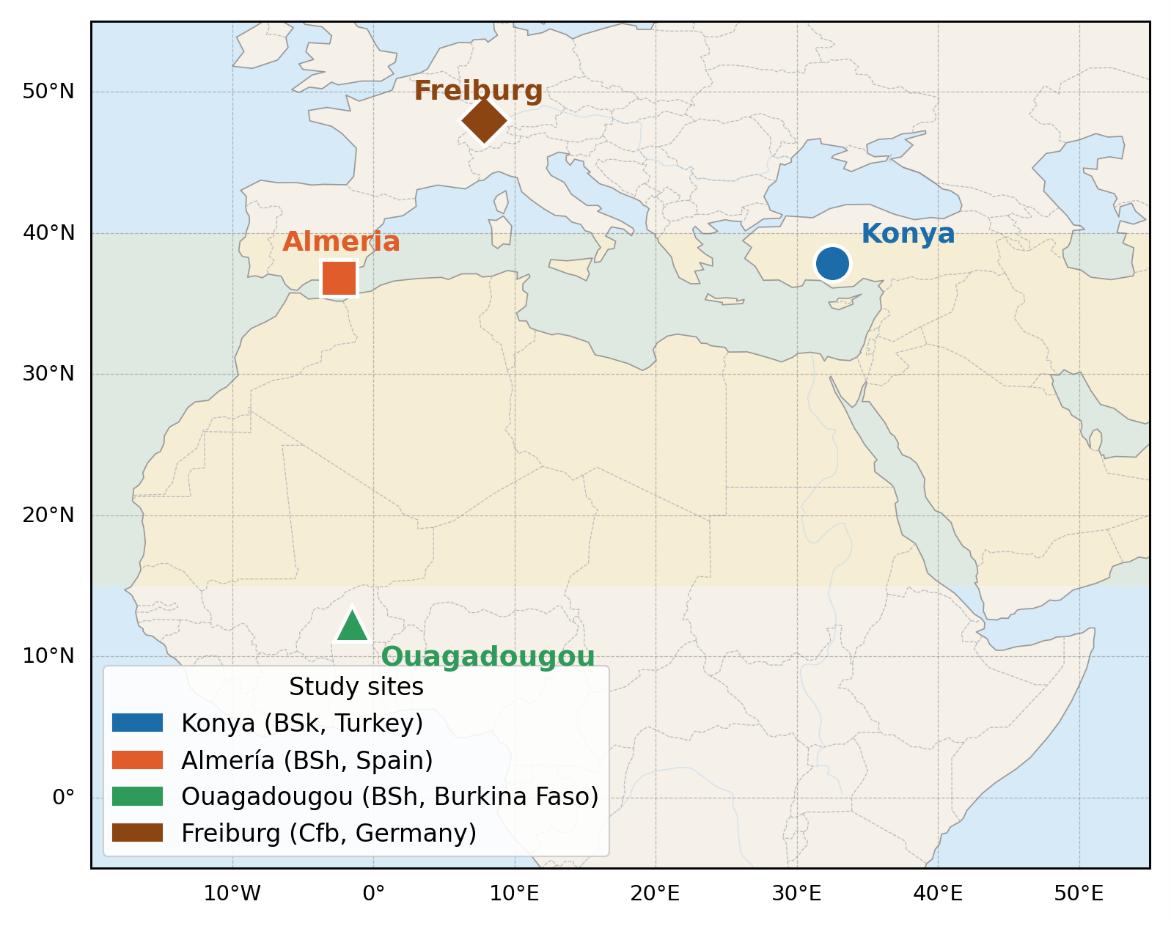
\includegraphics[width=\textwidth]{figures/fig01_site_map.png}
\caption{Location map of the four study sites overlaid on the
K\"{o}ppen--Geiger climate classification. Semi-arid zones (BS)
are shaded in light yellow; the oceanic temperate zone (Cfb) in
light blue.}
\label{fig:sitemap}
\end{figure}

Hourly climate data were obtained from the PVGIS-SARAH3 Typical
Meteorological Year (TMY) database of the European Commission Joint
Research Centre~\citep{pvgis, huld2012}. The SARAH3 satellite product
provides direct normal irradiance (DNI) and diffuse horizontal irradiance
(DHI) as independent retrievals, without decomposition from global
horizontal irradiance (GHI). This avoids the systematic decomposition
errors of up to $\pm$8\% reported for empirical decomposition models
under broken cloud conditions~\citep{urraca2017}. The mean bias error
of PVGIS-SARAH3 GHI estimates is below $\pm$5\% for monthly averages
at all four study sites~\citep{huld2012}. The TMY file format provides
ten meteorological variables at hourly resolution (8760 rows per site):
air temperature T$_{2m}$ (\si{\celsius}), relative humidity RH (\%),
GHI, DNI, DHI (W\,m$^{-2}$), downwelling infrared irradiance IR(h)
(W\,m$^{-2}$), 10-m wind speed WS$_{10m}$ (m\,s$^{-1}$), wind
direction WD$_{10m}$ (°), and surface pressure SP (Pa).

\begin{table}[H]
\caption{Geographical and climatic characteristics of the four study
sites (PVGIS-SARAH3 TMY data).}
\label{tab:sites}
\centering
\begin{tabular}{p{4cm}cccc}
\toprule
\textbf{Parameter} & \textbf{Konya} & \textbf{Almer\'{i}a}
    & \textbf{Ouagadougou} & \textbf{Freiburg} \\
\midrule
Latitude            & 37.87°N & 36.83°N & 12.37°N & 47.99°N \\
Longitude           & 32.49°E & 2.46°W  & 1.52°W  & 7.85°E  \\
Elevation (m a.s.l.)& 1\,016  & 20      & 303     & 278     \\
K\"{o}ppen class    & BSk     & BSh     & BSh     & Cfb     \\
Annual GHI (kWh\,m$^{-2}$) & 1\,650 & 1\,850 & 2\,050 & $\sim$1\,150 \\
Mean annual T (\si{\celsius}) & 11.5 & 18.5 & 28.5 & $\sim$11.4 \\
Summer T$_{\max}$ (\si{\celsius}) & 38 & 35 & 41 & $\sim$35 \\
Winter T$_{\min}$ (\si{\celsius}) & $-$10 & $+$5 & $+$15 & $\sim{-12}$ \\
Annual ET$_0$ (mm)  & 1\,200  & 1\,350  & 1\,800  & $\sim$900 \\
Annual precip. (mm) & 320     & 200     & 800     & $\sim$800 \\
\bottomrule
\end{tabular}
\end{table}

\begin{figure}[H]
\centering

\includegraphics[width=\textwidth]{figures/fig02_climate_profiles.png}
\caption{Monthly climate profiles for the four study sites from
PVGIS-SARAH3 TMY data. Upper row: monthly GHI (kWh\,m$^{-2}$)
with annual total annotated; lower row: mean monthly air temperature
(\si{\celsius}). Shaded bands indicate the tomato growing season
at each site.}
\label{fig:climateprofiles}
\end{figure}

The four sites span a mean annual temperature range of
11.4--28.5\,\si{\celsius}, a GHI range of 1\,150--2\,050\,kWh\,m$^{-2}$,
and growing seasons of 122--189 days. This diversity ensures that the
model is tested across the full range of Arrhenius BMP suppression
(from negligible at Ouagadougou to severe at Freiburg in January)
and PAR saturation regimes (from frequent saturation at Ouagadougou
to rare saturation at Freiburg), providing the basis for the
multi-climate findings reported in Section~\ref{sec:results}.

% ---------------------------------------------------------------------------
\subsection{Crop Parameters and Growing Seasons}
\label{sec:crop}
% ---------------------------------------------------------------------------

\hspace{1cm}Tomato (\textit{Solanum lycopersicum}) was selected as the
reference crop for all four sites on the basis of three criteria: it is
cultivated commercially in all four study regions, its PAR saturation
point (\SI{174}{W\,m^{-2}}) is well-documented and places it in the
high-irradiance sensitivity range where APV shading effects are most
pronounced, and its residue-to-fruit ratio and BMP are among the
best-characterised in the agrivoltaic and AD
literatures~\citep{mohammedi2023, lallement2023, feng2013}.

Site-specific planting and harvest dates follow local agricultural
calendars (Table~\ref{tab:crop}). The three semi-arid sites use a fresh
fruit yield of \SI{60}{t\,ha^{-1}}, consistent with irrigated greenhouse
and open-field production in Mediterranean and tropical semi-arid
contexts~\citep{mohammedi2023}. Freiburg uses \SI{30}{t\,ha^{-1}}
following German open-field production statistics~\citep{dlg2023}.

\begin{table}[H]
\caption{Site-specific agronomic, economic, and environmental parameters.
Grid emission factors (EF) from \citet{iea2025} and Umweltbundesamt (2023).
Carbon prices from EU ETS (2024) for Almer\'{i}a and Freiburg;
voluntary market rates for Konya and Ouagadougou.}
\label{tab:crop}
\centering
\begin{tabular}{lcccc}
\toprule
\textbf{Parameter} & \textbf{Konya} & \textbf{Almer\'{i}a}
    & \textbf{Ouagadougou} & \textbf{Freiburg} \\
\midrule
Planting date           & 25 Apr  & 1 Mar   & 1 Jul   & 1 May   \\
Harvest date            & 30 Oct  & 30 Jun  & 30 Oct  & 15 Oct  \\
Season length (days)    & 189     & 122     & 122     & 167     \\
Fruit yield (t\,ha$^{-1}$) & 60  & 60      & 60      & 30      \\
Season ET$_0$ (mm)      & 650     & 480     & 620     & $\sim$350 \\
Residue ratio $R_{\text{res}}$ & \multicolumn{4}{c}{0.80~\citep{mohammedi2023}} \\
Dry matter $DM$ (tomato residues) & \multicolumn{4}{c}{0.06~\citep{mohammedi2023}} \\
VS fraction $VS_f$      & \multicolumn{4}{c}{0.85~\citep{lallement2023}} \\
Manure input (t\,ha$^{-1}$\,yr$^{-1}$) & \multicolumn{4}{c}{10.0} \\
Manure $DM_m$           & \multicolumn{4}{c}{0.20~\citep{pilarski2025}} \\
Manure $VS_m$           & \multicolumn{4}{c}{0.80~\citep{pilarski2025}} \\
\midrule
Tomato price (\$\,t$^{-1}$) & 300 & 400  & 250     & 350     \\
Electricity price (\$\,kWh$^{-1}$) & 0.06 & 0.09 & 0.12 & 0.09 \\
Discount rate (\%)      & 8       & 6       & 10      & 5       \\
Grid EF (tCO$_2$\,MWh$^{-1}$) & 0.438 & 0.167 & 0.632 & 0.380 \\
Carbon price (\$\,tCO$_2^{-1}$) & 15  & 65    & 12      & 65      \\
\bottomrule
\end{tabular}
\end{table}

The feedstock to the anaerobic digester combines tomato crop residues
and cattle manure as a co-substrate. Manure co-digestion at a VS ratio
of approximately 1:2 (residues:manure) improves buffer capacity,
microbial diversity, and BMP by 12--18\% compared to mono-digestion of
crop residues alone~\citep{pilarski2025}. The \SI{10}{t\,ha^{-1}} fresh
manure input corresponds to the production of approximately 2--3 cattle
heads per hectare, consistent with the mixed crop-livestock farming
systems prevalent in all four study regions. Total annual VS input per
hectare is:
\begin{equation}
    VS_{\text{total}} =
    \underbrace{Y_f \cdot LER_{\text{crop}} \cdot
    R_{\text{res}} \cdot DM \cdot VS_f}_{\text{crop residues}}
    +\;
    \underbrace{M_m \cdot DM_m \cdot VS_m}_{\text{cattle manure}}
    \label{eq:vs}
\end{equation}
where $Y_f$ is the fresh fruit yield (kg\,ha$^{-1}$), $LER_{\text{crop}}$
scales the actual residue production under APV shading, and $M_m$
is the fresh manure input (kg\,ha$^{-1}$\,yr$^{-1}$). At the optimised
designs reported in Section~\ref{sec:results}, VS inputs range from
\SI{1892}{} to \SI{2573}{kg\,ha^{-1}\,yr^{-1}} across the four sites,
with Freiburg's lower fruit yield driving the minimum.

% ---------------------------------------------------------------------------
\subsection{Solar Geometry and Shading Model}
\label{sec:shading}
% ---------------------------------------------------------------------------

\hspace{1cm}Accurate hourly solar position calculation underpins both
the PV transposition model and the inter-row shading factor. Solar
declination $\delta$ is computed using the Spencer (1971) harmonic
approximation:
\begin{multline}
	\delta = \frac{180}{\pi}\Big(
	0.006918
	- 0.399912\cos B
	+ 0.070257\sin B \\
	- 0.006758\cos 2B
	+ 0.000907\sin 2B
	- 0.002697\cos 3B
	+ 0.001480\sin 3B
	\Big)
	\label{eq:declination}
\end{multline}
where $B = 2\pi(n-1)/365$ and $n$ is the day of year. The hour angle
$\omega$ is computed from true solar time, applying a longitude correction
and the Equation of Time. The solar elevation angle $\alpha_s$ at each
hourly timestep is:
\begin{equation}
    \sin\alpha_s = \sin\phi\sin\delta
        + \cos\phi\cos\delta\cos\omega
    \label{eq:elevation}
\end{equation}
where $\phi$ is the site latitude.

The Ground Coverage Ratio (GCR) quantifies the fraction of ground
area covered by the projected module footprint:
\begin{equation}
    GCR = \frac{L_m \cos\beta}{d_{\text{row}}}
    \label{eq:gcr}
\end{equation}
where $L_m = \SI{2.278}{m}$ is the module length (Jinko Tiger Neo
550\,W$_{\text{p}}$) and $\beta$ is the panel tilt angle. A physical
non-overlap constraint prevents adjacent rows from casting permanent
shade on each other at any sun angle:
\begin{equation}
    d_{\text{row}} \geq L_m\cos\beta + \SI{0.5}{m}
    \label{eq:overlap}
\end{equation}
where the \SI{0.5}{m} clearance accounts for module frame width and
structural tolerance. This constraint is enforced as a feasibility
penalty in the optimizer (Section~\ref{sec:optimizer}).

The hourly ground shading fraction $F_{\text{shad}}(t)$ --- the
fraction of ground area beneath the array that is shaded at time $t$
--- follows \citet{zainali2023}:
\begin{equation}
    F_{\text{shad}}(t) = \min\!\left(1,\;
    \frac{H_m\cos\Delta\gamma}
         {d_{\text{row}}\tan\alpha_s(t)}\right)
    \label{eq:shading}
\end{equation}
where $H_m$ is the module bottom-edge height above ground (m),
$\Delta\gamma$ is the azimuth difference between the solar direction
and the row orientation (zero for south-facing rows, which is the
configuration adopted throughout), and $\alpha_s(t)$ is the solar
elevation angle. $F_{\text{shad}} = 0$ at night ($\alpha_s \leq 0$)
and during high-sun periods when the solar elevation is sufficient
to eliminate inter-row shading entirely. The shading fraction directly
enters both the crop yield model (Section~\ref{sec:cropyield}) and
the ET reduction model (Section~\ref{sec:et}), propagating the
geometric design variables into all biological and energy outputs
of the coupled system.

% ---------------------------------------------------------------------------
\subsection{Photovoltaic Energy Model}
\label{sec:pvmodel}
% ---------------------------------------------------------------------------

\subsubsection{Plane-of-Array Irradiance}

\hspace{1cm}Plane-of-array (POA) irradiance on the tilted front surface
is computed using the isotropic sky model of \citet{liu1960}, which
decomposes incoming radiation into beam, diffuse, and ground-reflected
components:
\begin{equation}
    G_{\text{front}} = DNI\cos\theta_i
        + DHI\frac{1+\cos\beta}{2}
        + GHI\,\rho_g\frac{1-\cos\beta}{2}
    \label{eq:poa}
\end{equation}
where $\theta_i$ is the angle of incidence on the tilted surface,
$\beta$ is the panel tilt angle, and $\rho_g = 0.25$ is the ground
albedo~\citep{monteith2008}. The angle of incidence for a fixed,
due-south-facing tilted surface is given by the closed-form
expression of \citet{duffie2013}, expressed directly in terms of
declination $\delta$, latitude $\phi$, hour angle $\omega$, and
tilt $\beta$:
\begin{equation}
    \cos\theta_i = \sin\delta\sin(\phi-\beta)
        + \cos\delta\cos\omega\cos(\phi-\beta)
    \label{eq:aoi}
\end{equation}
This expression is exact for a fixed due-south collector at every
hour of the day. An earlier version of this model used the
solar-noon-only approximation
$\cos\theta_i \approx \sin\alpha_s\cos\beta + \cos\alpha_s\sin\beta$,
which implicitly assumes the sun remains due south throughout the
day; this systematically overestimated front-surface beam
irradiance away from solar noon and has been corrected throughout
the present study.

For bifacial modules, rear-side irradiance $G_{\text{rear}}$ is
estimated from ground-reflected radiation modulated by the inter-row
shading fraction:
\begin{equation}
    G_{\text{rear}} = GHI\,\rho_g
        \left(1 - F_{\text{shad}}(t)\right)\,f_{\text{rear}}
    \label{eq:grear}
\end{equation}
where $f_{\text{rear}} = 0.12$ is the rear irradiance fraction
relative to ground-reflected GHI, accounting for the view factor
from the rear surface to the ground beneath the
array~\citep{gorjian2022}. The effective bifacial irradiance
combining both surfaces is:
\begin{equation}
    G_{\text{eff}} = G_{\text{front}}
        + \phi\,G_{\text{rear}}
    \label{eq:geff}
\end{equation}
where $\phi = 0.70$ is the bifaciality factor of the Jinko Tiger
Neo 550\,W$_{\text{p}}$ module.

\subsubsection{Cell Temperature}

\hspace{1cm}Cell operating temperature is modelled using the
Faiman~\citep{faiman2008} approach, which accounts for
wind-dependent convective cooling:
\begin{equation}
    T_{\text{cell}}(t) = T_{\text{amb}}(t)
        + \frac{G_{\text{eff}}(t)}{U_0 + U_1\,u(t)}
    \label{eq:tcell}
\end{equation}
where $U_0 = \SI{25}{W\,m^{-2}\,K^{-1}}$ is the free convection
coefficient and $U_1 = \SI{6.84}{W\,s\,m^{-3}\,K^{-1}}$ is the
wind-dependent convective coefficient~\citep{faiman2008}.
Wind speed $u(t)$ is taken directly from the PVGIS-SARAH3 TMY
column WS$_{10m}$ and clipped to a minimum of
\SI{0.5}{m\,s^{-1}} to prevent division by zero in calm
conditions.

\subsubsection{PV Power Output}

\hspace{1cm}Array power output at each hourly timestep is:
\begin{equation}
    P_{\text{PV}}(t) = P_{\text{STC}}\,N\,(1-\eta_{\text{loss}})
        \left[1 + \beta_p\left(T_{\text{cell}}(t) - 25\right)\right]
        \frac{G_{\text{eff}}(t)}{1000}
    \label{eq:ppv}
\end{equation}
where $P_{\text{STC}} = \SI{550}{W_p}$ is the rated module power
at Standard Test Conditions, $N$ is the number of modules per
hectare (determined by $\beta$ and $d_{\text{row}}$ via
Equation~\ref{eq:gcr}), $\eta_{\text{loss}} = 0.12$ aggregates
all system losses (wiring, soiling, mismatch, inverter), and
$\beta_p = \SI{-0.0035}{K^{-1}}$ is the temperature power
coefficient~\citep{jinko}. Annual PV energy is partitioned
between grid export and digester heating:
\begin{align}
    E_{\text{PV,heat}} &= f_{\text{PV,heat}} \times E_{\text{PV,total}} \\
    E_{\text{PV,sold}} &= (1 - f_{\text{PV,heat}}) \times E_{\text{PV,total}}
    \label{eq:pvpartition}
\end{align}
where $f_{\text{PV,heat}} \in [0.05,\,0.50]$ is the sixth design
variable optimised by the DE algorithm. Table~\ref{tab:pvparams}
summarises all fixed PV model parameters.

\begin{table}[H]
\caption{Fixed PV model parameters.}
\label{tab:pvparams}
\centering
\begin{tabular}{llll}
\toprule
\textbf{Parameter} & \textbf{Symbol} & \textbf{Value} & \textbf{Source} \\
\midrule
Rated power (STC)       & $P_{\text{STC}}$ & 550\,W$_p$          & \citet{jinko} \\
Module length           & $L_m$            & 2.278\,m            & \citet{jinko} \\
Bifaciality factor      & $\phi$           & 0.70                & \citet{jinko} \\
Temp. coefficient       & $\beta_p$        & $-$0.0035\,K$^{-1}$ & \citet{jinko} \\
System losses           & $\eta_{\text{loss}}$ & 0.12            & \citet{jordan2013} \\
Ground albedo           & $\rho_g$         & 0.25                & \citet{monteith2008} \\
Faiman $U_0$            & $U_0$            & 25\,W\,m$^{-2}$\,K$^{-1}$ & \citet{faiman2008} \\
Faiman $U_1$            & $U_1$            & 6.84\,W\,s\,m$^{-3}$\,K$^{-1}$ & \citet{faiman2008} \\
Rear irradiance fraction & $f_{\text{rear}}$ & 0.12             & \citet{gorjian_progress_2022} \\
\bottomrule
\end{tabular}
\end{table}

% ---------------------------------------------------------------------------
\subsection{Crop Yield Model}
\label{sec:cropyield}
% ---------------------------------------------------------------------------

\hspace{1cm}Relative crop yield is modelled using the PAR integral
method, which integrates the gap between available and saturating
photosynthetically active radiation over the growing season. The fraction
of global horizontal irradiance that is photosynthetically active
is $f_{\text{PAR}} = 0.48$~\citep{mccree1971, jacovides2006}. Hourly
PAR under the APV array and in an equivalent open field are:
\begin{align}
    PAR_{\text{AV}}(t)   &= GHI(t) \times f_{\text{PAR}}
        \times \bigl(1 - F_{\text{shad}}(t)\bigr)
        \label{eq:parav} \\
    PAR_{\text{open}}(t) &= GHI(t) \times f_{\text{PAR}}
        \label{eq:paropen}
\end{align}

The tomato light saturation point is
$PAR_{\text{sat}} = \SI{174}{W\,m^{-2}}$~\citep{mohammedi2023,
heuvelink2005}, above which additional PAR delivers no incremental
photosynthesis. The annual yield ratio, integrated exclusively over
the growing season $[t_0,\,t_1]$, is:
\begin{equation}
    LER_{\text{crop}}
        = \frac{\displaystyle\int_{t_0}^{t_1}
                \min\!\bigl(PAR_{\text{AV}}(t),\;PAR_{\text{sat}}\bigr)\,dt}
               {\displaystyle\int_{t_0}^{t_1}
                PAR_{\text{open}}(t)\,dt}
    \label{eq:lercrop}
\end{equation}

Three properties of Equation~\ref{eq:lercrop} are worth noting
explicitly. First, $LER_{\text{crop}}$ is bounded above by 1.0: the
APV array cannot increase crop yield beyond the open-field reference
in the absence of heat stress or water limitation effects, which are
not modelled here. Second, at high irradiance sites where
$PAR_{\text{open}}(t) \gg PAR_{\text{sat}}$ for a large fraction of
daytime hours, the denominator is large relative to the numerator
even before any shading is applied, making $LER_{\text{crop}}$
sensitive to the ratio $PAR_{\text{sat}}/\overline{PAR_{\text{open}}}$
--- the mechanism that drives the non-monotone eLER--GHI relationship
identified in Section~\ref{sec:results}. Third, integration is
performed over the growing season only: including off-season hours
(when $GHI \approx 0$ at night and both integrals are zero) does not
change the ratio, but restricting to $[t_0,\,t_1]$ correctly attributes
yield impacts to the period when the crop is actually present.

Model validation against the six-point shading dataset of
\citet{mohammedi2023} is reported in Section~\ref{sec:validation}
(V1 validation, MAPE = 2.4\% in the operational shading range
$F_{\text{shad}} \leq 0.25$).

% ---------------------------------------------------------------------------
\subsection{Evapotranspiration Reduction and Water Savings}
\label{sec:et}
% ---------------------------------------------------------------------------

\hspace{1cm}Reference evapotranspiration ET$_0$ is estimated hourly
using the Hargreaves--Samani equation~\citep{hargreaves1985}, driven
by the daily temperature range and extraterrestrial radiation $R_a$
computed astronomically from latitude and day of year following the
standard FAO-56 formulation~\citep{allen1998}, requiring no ground
radiation measurement. The Hargreaves--Samani method was
selected over FAO-56 Penman-Monteith~\citep{allen1998} because the
PVGIS TMY files do not provide dew point temperature or net radiation
as independent columns, making two of the four Penman-Monteith inputs
unavailable without auxiliary decomposition. Hargreaves--Samani
estimates of seasonal ET$_0$ agree with FAO-56 to within $\pm$10\%
for the semi-arid and temperate climates represented in this
study~\citep{droogers2002}.

Under APV panels, evapotranspiration is reduced by the interception
of incoming radiation. Following \citet{elamri2018} and
\citet{tawassulli2025}, the hourly ET under the APV array is:
\begin{equation}
    ET_{\text{APV}}(t) = ET_0(t)
        \times \bigl(1 - \alpha_{\text{shade}}\,F_{\text{shad}}(t)\bigr)
    \label{eq:etapv}
\end{equation}
where $\alpha_{\text{shade}} = 0.40$ is the ET reduction coefficient,
empirically calibrated from field measurements of soil evaporation
and canopy transpiration under partial shade~\citep{elamri2018,
tawassulli2025}. The value $\alpha_{\text{shade}} = 0.40$ represents
a conservative central estimate; field studies at GCR $>$ 0.5 report
values of 0.35--0.55 depending on crop canopy closure, soil type, and
wind exposure. Sensitivity to $\alpha_{\text{shade}}$ is discussed in
Section~\ref{sec:discussion}.

Annual growing-season water savings are:
\begin{equation}
    W_{\text{saved}} = \int_{t_0}^{t_1}
        \bigl[ET_0(t) - ET_{\text{APV}}(t)\bigr]\,dt
        = \alpha_{\text{shade}}\int_{t_0}^{t_1}
        F_{\text{shad}}(t)\,ET_0(t)\,dt
    \label{eq:wsaved}
\end{equation}

The water savings Land Equivalent Ratio is defined as the fraction
of growing-season ET$_0$ saved by the APV system:
\begin{equation}
    LER_{\text{water}} =
        \frac{W_{\text{saved}}}
             {\displaystyle\int_{t_0}^{t_1} ET_0(t)\,dt}
        \times 100\%
    \label{eq:lerwater}
\end{equation}

\textbf{Note on the denominator.} Prior agrivoltaic studies
have reported $LER_{\text{water}}$ using annual ET$_0$ as the
denominator~\citep{barron2019, elamri2018}, systematically
underestimating the agronomic benefit by diluting growing-season
savings with months when the crop is absent and the panels provide
no agronomic water benefit. With a 122-day season (Almer\'{i}a,
Ouagadougou), the annual denominator inflates by a factor of
$365/122 = 3.0$ relative to the growing-season denominator,
reducing the reported $LER_{\text{water}}$ by the same factor.
The correction is largest at Almer\'{i}a and Ouagadougou (factor
3.0) and smallest at Konya (factor 1.9, 189-day season). Throughout
this paper, $LER_{\text{water}}$ uses the growing-season denominator
(Equation~\ref{eq:lerwater}); the annual-denominator value is
reported alongside for literature comparison only.

% ---------------------------------------------------------------------------
\subsection{Anaerobic Digestion Model}
\label{sec:admodel}
% ---------------------------------------------------------------------------

\subsubsection{Effective Digester Temperature}

\hspace{1cm}The effective digester operating temperature is determined
by the ambient temperature profile and the thermal management strategy.
PV electricity allocated to resistive heating ($f_{\text{PV,heat}}$
fraction of annual PV output) maintains the digester above a minimum
operating threshold. The effective digester temperature is modelled as:
\begin{equation}
	T_{\text{dig,eff}} = \mathrm{clip}
	\!\left(T_{\text{amb,monthly}} + 5,\;
	T_{\text{min}},\; T_{\text{ref}}\right)
	\label{eq:tdig}
\end{equation}
where $T_{\text{min}} = \SI{26}{\celsius}$ is the minimum acceptable
operating temperature below which methanogenesis becomes severely
inhibited, $T_{\text{ref}} = \SI{37}{\celsius}$ is the mesophilic
optimum, and the $+5\,^{\circ}$C boost above monthly mean ambient
temperature represents the passive thermal gain from digester
insulation and exothermic reaction heat~\citep{lindorfer2008}.
Monthly mean ambient temperatures from the PVGIS-SARAH3 TMY are
used as the seasonal driver, reflecting the thermal inertia of a
well-insulated CSTR digester that equilibrates on a monthly rather
than hourly timescale.

\subsubsection{Arrhenius BMP Temperature Correction}

\hspace{1cm}The temperature-corrected biochemical methane potential
follows an Arrhenius-type relationship~\citep{pilarski2025, feng2013}:
\begin{equation}
	BMP(T_{\text{dig,eff}}) = BMP_{\text{ref}} \times
	\exp\!\bigl[\theta\,
	(T_{\text{dig,eff}} - T_{\text{ref}})\bigr]
	\label{eq:bmp}
\end{equation}
with reference BMP $BMP_{\text{ref}} = \SI{300}{NmL\,CH_4\,gVS^{-1}}$
at $T_{\text{ref}} = \SI{37}{\celsius}$ and Arrhenius coefficient
$\theta = \SI{0.069}{\celsius^{-1}}$~\citep{pilarski2025}. Annual
methane production is:
\begin{equation}
	V_{\text{CH}_4} = VS_{\text{total}} \times
	\overline{BMP} \times \eta_{\text{cap}}
	\label{eq:ch4vol}
\end{equation}
where $\overline{BMP}$ is the annual average BMP weighted by monthly
VS throughput, $\eta_{\text{cap}} = 1.00$ under baseline conditions
(S0), and $VS_{\text{total}}$ is from Equation~\ref{eq:vs}.
Annual biogas energy is:
\begin{equation}
	E_{\text{biogas}} = V_{\text{CH}_4} \times
	f_{\text{CH}_4} \times LHV_{\text{CH}_4}
	\label{eq:ebiogas}
\end{equation}
with methane fraction $f_{\text{CH}_4} = 0.60$ and lower heating
value $LHV_{\text{CH}_4} = \SI{35.8}{MJ\,Nm^{-3}}$~\citep{marchaim1992}.
Validation of the BMP temperature model against the five-point
experimental dataset of \citet{feng2013} is reported in
Section~\ref{sec:validation} (V2 validation,
MAPE = 26.9\% in the operating range $T \leq \SI{37}{\celsius}$).
Sensitivity of biogas output and eLER to $BMP_{\text{ref}}$,
capture efficiency $\eta_{\text{cap}}$, and volatile-solids
fractions is assessed via Monte Carlo sampling over
literature-reported ranges in Section~\ref{sec:discussion}.

\subsubsection{Digester Heat Balance}

\hspace{1cm}The annual digester heat demand is the sum of conductive
wall losses, substrate heating requirement, and the exothermic
reaction credit~\citep{pal2024}:
\begin{equation}
	Q_{\text{heat}} = Q_{\text{loss}} + Q_{\text{inflow}}
	- Q_{\text{reaction}}
	\label{eq:qheat}
\end{equation}

Conductive wall losses from a cylindrical digester (height = diameter
assumption) with effective heat transfer coefficient
$U_{\text{eff}} = \SI{0.8}{W\,m^{-2}\,K^{-1}}$~\citep{lindorfer2008}:
\begin{equation}
	Q_{\text{loss}} = U_{\text{eff}}\,A_{\text{wall}}
	\left(\overline{T}_{\text{dig}} - \overline{T}_{\text{amb}}\right)
	\times \frac{8760}{1000}
	\label{eq:qloss}
\end{equation}
where $A_{\text{wall}}$ is the total digester surface area (m$^2$)
and the factor $8760/1000$ converts from W to MWh\,yr$^{-1}$.
Substrate heating demand:
\begin{equation}
	Q_{\text{inflow}} = \frac{V_{\text{dig}}}{HRT}
	\times 365 \times \rho_s \times C_p
	\times \max\!\left(0,\,
	\overline{T}_{\text{dig}} - T_{\text{in}}\right)
	/ 3600
	\label{eq:qinflow}
\end{equation}
with substrate density $\rho_s = \SI{1020}{kg\,m^{-3}}$, specific
heat $C_p = \SI{4.2}{kJ\,kg^{-1}\,K^{-1}}$, and inlet temperature
$T_{\text{in}} = \SI{15}{\celsius}$. The exothermic reaction credit
is estimated as 5\% of gross biogas energy~\citep{pal2024}:
\begin{equation}
	Q_{\text{reaction}} = 0.05 \times E_{\text{biogas}}
	\label{eq:qreaction}
\end{equation}

\subsubsection{Energy Self-Sufficiency Ratio}

\hspace{1cm}The Energy Self-sufficiency Ratio quantifies the thermal
margin of the integrated system:
\begin{equation}
	ESR = \frac{E_{\text{PV,total}} + E_{\text{biogas}}}
	{Q_{\text{heat}}}
	\label{eq:esr}
\end{equation}
When $ESR \gg 1$, the combined PV and biogas output far exceeds
the digester heating requirement, and zero biogas is consumed for
self-heating. Under this condition, $LER_{\text{biogas}}$ equals
the ratio of APV-system biogas to open-field reference biogas
by construction --- a structural identity rather than an optimised
outcome, as discussed in Section~\ref{sec:discussion}.

% ---------------------------------------------------------------------------
\subsection{Extended Land Equivalent Ratio}
\label{sec:eler}
% ---------------------------------------------------------------------------

\hspace{1cm}The extended Land Equivalent Ratio (eLER) generalises the
classical two-component agrivoltaic LER by adding net biogas energy as
a third dimensionless land-use output:
\begin{equation}
	eLER =
	\underbrace{\frac{Y_{\text{crop,AV}}}{Y_{\text{crop,open}}}}_{LER_{\text{crop}}}
	+
	\underbrace{\frac{E_{\text{PV,sold}}}{E_{\text{PV,ref}}}}_{LER_{\text{PV}}}
	+
	\underbrace{\frac{E_{\text{biogas,APV}}}{E_{\text{biogas,ref}}}}_{LER_{\text{biogas}}}
	\label{eq:eler}
\end{equation}

An eLER greater than 1.0 confirms that the integrated APV--AD system
uses land more productively than three separate monocultures --- an
open-field crop, a dense-pack ground-mount PV array, and a standalone
AD unit --- occupying the same total area. Equal weighting of the
three components is adopted here, consistent with the original
two-component LER framework, in which each term is already normalised
to its own reference system and is therefore commensurable without
further weighting; the sensitivity of eLER and cross-site rankings
to alternative (energy-content- and revenue-weighted) schemes is
examined in Section~\ref{sec:discussion}. Each component is defined
as follows.

\textbf{$LER_{\text{crop}}$} is the yield ratio from
Equation~\ref{eq:lercrop}: the ratio of growing-season PAR integral
under the APV array to the open-field PAR integral, bounded in
$[0,\,1]$ for tomato at the modelled irradiance levels.

\textbf{$LER_{\text{PV}}$} is the ratio of annual APV electricity
sold to grid to the reference PV output. Two reference definitions
are used:

\begin{itemize}[leftmargin=*, noitemsep]
	\item \textbf{Definition A (independent reference, primary)}: 
	$E_{\text{PV,ref}}$ is computed from a simulated dense-pack
	ground-mount array at the same tilt angle $\beta^*$ with no
	inter-row shading (GCR = 1.0 in the limiting sense, i.e.\ rows
	spaced at exactly the module projected width $L_m\cos\beta$).
	This provides a rigorous, non-circular reference that is
	independent of the APV design variables.
	
	\item \textbf{Definition B (circular reference, for comparison)}:
	$LER_{\text{PV}} \equiv GCR$, as the APV array output referenced
	to itself equals the fraction of ground covered. Reported for
	literature comparability with studies using this convention, but
	not used as the primary metric~\citep{mazzeo2025}.
\end{itemize}

\textbf{$LER_{\text{biogas}}$} is the ratio of biogas energy produced
by the APV--AD system to the output of a standalone reference AD unit.
The reference AD unit processes the same land area under open-field
conditions ($LER_{\text{crop}} = 1.0$, maximum residue production)
with identical digester volume, HRT, and manure co-substrate:
\begin{equation}
	LER_{\text{biogas}} =
	\frac{E_{\text{biogas,APV}}}{E_{\text{biogas,ref}}}
	\label{eq:lerbiogas}
\end{equation}
Because the manure co-substrate ($VS_{\text{manure}}$) is identical
in both the APV and reference cases, $LER_{\text{biogas}}$ reflects
exclusively the effect of APV shading on crop residue production.
When $LER_{\text{crop}} < 1$, the APV system produces fewer crop
residues than the open-field reference, and consequently
$LER_{\text{biogas}} < 1$. This is a structural consequence of
the shading-residue coupling, not a model artefact.

The two-component benchmark for literature comparison is:
\begin{equation}
	LER_{\text{2C}} = LER_{\text{crop}} + LER_{\text{PV}}(\text{Def.~A})
	\label{eq:ler2c}
\end{equation}
The published two-component maximum is $LER_{\text{2C}} = 1.94$
from \citet{riaz2022} for bifacial tomato in Arizona. All results in
this study are reported under Definition~A unless explicitly stated
otherwise, and the numerical difference between Definition~A and~B
is reported in Table~\ref{tab:eLER}.

% ---------------------------------------------------------------------------
\subsection{Design Optimization}
\label{sec:optimizer}
% ---------------------------------------------------------------------------

\subsubsection{Differential Evolution Algorithm}

\hspace{1cm}The six design variables and their bounds are summarised in
Table~\ref{tab:bounds}. The objective function $eLER(\mathbf{x})$
(Equation~\ref{eq:eler}) is maximised using Differential Evolution
(DE)~\citep{storn1997}, a population-based global optimizer that
requires no gradient information and handles non-smooth, multimodal
objective landscapes efficiently. DE has been widely applied to
renewable energy system sizing problems where the design space
contains bound constraints and discrete-continuous
interactions~\citep{oprea2024}.

\begin{table}[H]
	\caption{Design variable bounds for Differential Evolution.
		The inter-row clearance constraint (Equation~\ref{eq:overlap})
		is enforced dynamically as a feasibility penalty during optimization.}
	\label{tab:bounds}
	\centering
	\begin{tabular}{llccl}
		\toprule
		\textbf{Variable} & \textbf{Symbol}
		& \textbf{Lower} & \textbf{Upper} & \textbf{Unit} \\
		\midrule
		Panel tilt angle          & $\beta$              & 15  & 40   & ° \\
		Row spacing               & $d_{\text{row}}$     & 3   & 14   & m \\
		Module bottom-edge height & $H_m$                & 1.5 & 5.0  & m \\
		Digester volume           & $V_{\text{dig}}$     & 2   & 50   & m³ \\
		Hydraulic retention time  & $HRT$                & 20  & 40   & days \\
		PV heating fraction       & $f_{\text{PV,heat}}$ & 0.05& 0.50 & --- \\
		\bottomrule
	\end{tabular}
\end{table}

The DE configuration follows established best-practice
recommendations~\citep{storn1997, das2011}:

\begin{itemize}[leftmargin=*, noitemsep]
	\item Population size: $NP = 15 \times n_{\text{var}} = 90$
	individuals, initialised via Latin Hypercube Sampling
	with seed = 42 for reproducibility.
	\item Mutation factor: $F$ dithered uniformly in $[0.5,\,1.0]$
	at each generation, balancing global exploration with
	local convergence.
	\item Crossover probability: $Cr = 0.70$ (binomial crossover).
	\item Maximum generations: $G_{\max} = 50$.
	\item Local polishing: after DE convergence, the best candidate
	is refined using L-BFGS-B with bound constraints,
	recovering sub-pixel precision in the continuous
	design space.
\end{itemize}

Two feasibility constraints are enforced via an infeasibility
penalty $f = -\infty$ applied to violating candidates:
\begin{enumerate}[leftmargin=*, noitemsep]
	\item Organic loading rate: $OLR \in
	[1.5,\;5.0]\;\text{kg\,VS\,m}^{-3}\text{d}^{-1}$,
	ensuring stable digester operation without
	acidification or underloading.
	\item Inter-row clearance:
	$d_{\text{row}} \geq L_m\cos\beta + \SI{0.5}{m}$,
	preventing physical module overlap
	(Equation~\ref{eq:overlap}).
\end{enumerate}

The complete pseudocode of the DE procedure is given in
Appendix~\ref{app:de}. Each evaluation of the objective function
$eLER(\mathbf{x})$ runs the full six-model pipeline --- solar
geometry, PV model, crop yield, ET reduction, AD model, and eLER
assembly --- on the 8760-hour TMY dataset for the corresponding
site. At $NP = 90$ individuals and $G_{\max} = 50$ generations,
each site requires $90 \times 50 = 4500$ full pipeline evaluations,
converging in 102--172 seconds on a standard desktop CPU.

\subsubsection{Boundary Convergence}
\label{sec:boundaryconv}

\hspace{1cm}At all four sites, the optimizer converges to the
lower bounds of row spacing ($d_{\text{row}}^* = \SI{3.03}{m}$,
constrained by the inter-row clearance condition) and module
height ($H_m^* = \SI{1.50}{m}$, the specified lower bound).
This boundary convergence is a structural result: the eLER
landscape has its global maximum at the physical constraint
boundary, where maximum panel density simultaneously maximises
PV output and reduces the open-field PAR integral denominator
(Equation~\ref{eq:lercrop}). The L-BFGS-B polishing step
confirms that no interior local maximum exists in the neighbourhood
of the boundary solution. The eLER penalty associated with any
mechanical access requirement beyond the minimum clearance is
quantified in the sensitivity analysis of
Section~\ref{sec:discussion}.

\subsubsection{Multi-Objective Extension (NSGA-II)}

\hspace{1cm}For the water trade-off analysis, the scalar eLER
objective is replaced by a bi-objective problem: simultaneously
maximise $eLER$ and $LER_{\text{water}}$ (Equation~\ref{eq:lerwater}).
This is solved using NSGA-II~\citep{blank2020} with 50 solutions
and 80 generations implemented via the \texttt{pymoo}
library~\citep{blank2020}. The bi-objective Pareto front provides
the decision-maker with explicit trade-off information between
land productivity and water conservation, enabling context-specific
design choices for water-stressed smallholder systems.

% ---------------------------------------------------------------------------
\subsection{AD Valorization Scenarios}
\label{sec:scenarios}
% ---------------------------------------------------------------------------

\hspace{1cm}Seven economic scenarios (S0--S6) are evaluated to quantify
the sensitivity of project economics to biogas valorization strategy and
carbon market participation (Table~\ref{tab:scenarios}). All scenarios
share the same optimized APV--AD design ($\mathbf{x}^*$) and differ
only in biogas price, BMP multiplier, capture efficiency, or additional
revenue streams. eLER is invariant across scenarios by construction,
since it depends solely on physical outputs ($E_{\text{PV,sold}}$,
$Y_{\text{crop}}$, $E_{\text{biogas}}$) and not on market prices.

\begin{table}[H]
	\caption{AD valorization scenarios S0--S6. All scenarios use the
		same optimized design $\mathbf{x}^*$. eLER is identical across
		scenarios; only revenue structure changes.}
	\label{tab:scenarios}
	\centering
	\begin{tabular}{lp{5.5cm}l}
		\toprule
		\textbf{Scenario} & \textbf{Description} & \textbf{Key modification} \\
		\midrule
		S0 & Baseline: mono-digestion, 100\% grid export
		& $BMP_{\text{mult}} = 1.00$,\ $\eta_{\text{cap}} = 1.00$ \\
		S1 & Co-digestion: $+$30\% cattle manure
		& $BMP_{\text{mult}} = 1.15$ \\
		S2 & Sub-optimal CH$_4$ capture (85\%)
		& $\eta_{\text{cap}} = 0.85$ \\
		S3 & LPG displacement (on-site use)
		& $p_{\text{bg}} = \$0.18\,\text{kWh}^{-1}$ \\
		S4 & Digestate N--P--K credit
		& N credit at $\$1.20\,\text{kg}^{-1}$ N \\
		S5 & Biomethane grid injection (EU premium)
		& $p_{\text{bg}} = 5.5\,p_{\text{elec}}$ \\
		S6 & Carbon credit (voluntary market)
		& $p_c$ = site-specific (\$/tCO$_2$) \\
		\bottomrule
	\end{tabular}
\end{table}

\textbf{Scenario S0} serves as the economic baseline: biogas is sold
at the local grid biogas tariff $p_{\text{bg}}$ (Table~\ref{tab:crop})
and all PV electricity is exported to grid at $p_{\text{elec}}$
after deducting the heating fraction $f_{\text{PV,heat}}$.

\textbf{Scenario S1} models co-digestion with a 30\% increase in
cattle manure beyond the baseline co-substrate, raising BMP by 15\%
through improved C:N ratio and microbial
diversity~\citep{pilarski2025}. The additional manure input is
assumed available at zero marginal cost from the same farm herd.

\textbf{Scenario S2} models sub-optimal biogas capture at 85\%
efficiency, representing a system with gas leakage, flaring, or
insufficient gas storage. It provides a lower bound on the biogas
revenue stream.

\textbf{Scenario S3} models on-site LPG displacement, where biogas
is used directly for cooking or process heat at a price parity of
\$0.18\,kWh$^{-1}$ --- the average LPG equivalent price in the four
study regions~\citep{iea2025}. This scenario is particularly
relevant for Ouagadougou, where LPG import costs are high.

\textbf{Scenario S4} adds a digestate nitrogen credit of
\$1.20\,kg$^{-1}$\,N, reflecting the avoided cost of equivalent
synthetic urea fertilizer. Digestate N content is estimated as
$0.003\,\text{kg\,N}\,\text{kg}^{-1}$ fresh
residue~\citep{lallement2023}.

\textbf{Scenario S5} models biomethane grid injection under European
EEG 2023 and RED III incentives, where the effective biomethane
market price is $5.5\times$ the local electricity purchase
price~\citep{nikzad2026, eba2025, rabobank2025}. This scenario is
directly applicable to Almer\'{i}a and Freiburg; for Konya and
Ouagadougou, which lack biomethane grid injection policy frameworks,
S5 represents an aspirational upper bound pending regulatory
development.

\textbf{Scenario S6} adds a carbon credit revenue stream based on
CO$_2$ displaced by PV electricity and biogas substituting fossil
fuels. Carbon prices are site-specific: EU ETS market rate
(\$65\,tCO$_2^{-1}$) for Almer\'{i}a and Freiburg; voluntary Gold
Standard rate (\$12\,tCO$_2^{-1}$) for Ouagadougou; and Turkish
voluntary carbon market rate (\$15\,tCO$_2^{-1}$) for Konya.
Annual CO$_2$ avoidance is:
\begin{equation}
	CO_{2,\text{avoided}} =
	E_{\text{PV,sold}} \times EF_{\text{grid}}
	+ \frac{E_{\text{biogas}}}{1000}
	\times EF_{\text{gas}}
	\label{eq:co2}
\end{equation}
where $EF_{\text{grid}}$ is the site-specific grid emission factor
(Table~\ref{tab:crop}) and $EF_{\text{gas}} =
\SI{0.202}{tCO_2\,MWh^{-1}}$ is the natural gas emission factor
from IPCC AR6~\citep{ipcc2022}.
% ---------------------------------------------------------------------------
\subsection{4E Analysis Framework}
\label{sec:4e}
% ---------------------------------------------------------------------------

\hspace{1cm}Investment-grade economic evaluation uses a 20-year project
life with site-specific discount rates (Table~\ref{tab:crop}), annualized
CAPEX, and annual O\&M fixed at 1.5\% of total CAPEX. The 4E framework
integrates four performance dimensions into a single comparative
assessment across sites and scenarios.

\subsubsection{E1 --- Energetic Analysis}

\hspace{1cm}The energetic dimension quantifies annual energy flows:
PV total generation, PV sold to grid, biogas energy, digester heat
demand, and ESR (Equation~\ref{eq:esr}). These are reported per
hectare of land area for cross-site comparability.

\subsubsection{E2 --- Economic Analysis}

\hspace{1cm}CAPEX is decomposed into four components:
\begin{itemize}[leftmargin=*, noitemsep]
	\item \textbf{PV array} (elevated APV structure):
	\$0.63\,W$_p^{-1}$, reflecting the \$0.45\,W$_p^{-1}$
	utility-scale ground-mount benchmark~\citep{irena2022}
	plus a 40\% premium for elevated APV mounting structure,
	cable routing, and installation.
	\item \textbf{AD digester}: \$800\,m$^{-3}$ installed
	capacity~\citep{pal2024}, covering tank construction,
	mixing system, gas handling, and instrumentation for
	small farm-scale CSTR digesters (2--50\,m$^3$).
	\item \textbf{Agricultural infrastructure}: \$2\,500\,ha$^{-1}$
	(FAO benchmark), covering drip irrigation installation,
	soil preparation, and access tracks.
	\item \textbf{Balance of plant (BOP)}: 15\% of (PV + AD) CAPEX,
	covering inverters, electrical wiring, civil works,
	and commissioning.
\end{itemize}

Annual gross revenue combines all income streams active under the
relevant scenario:
\begin{equation}
	R_{\text{gross}} = R_{\text{PV}} + R_{\text{tomato}}
	+ R_{\text{biogas}} + R_{\text{digestate}}
	+ R_{\text{carbon}}
	\label{eq:revenue}
\end{equation}

Net annual cash flow, Net Present Value, Internal Rate of Return,
and simple payback period are:
\begin{align}
	CF_{\text{net}} &= R_{\text{gross}} - C_{\text{O\&M}}
	\label{eq:cf} \\[4pt]
	NPV &= -CAPEX + CF_{\text{net}}
	\times \frac{1-(1+r)^{-N}}{r}
	\label{eq:npv} \\[4pt]
	IRR &: \quad 0 = -CAPEX + CF_{\text{net}}
	\times \frac{1-(1+IRR)^{-N}}{IRR}
	\label{eq:irr} \\[4pt]
	PB &= \frac{CAPEX}{CF_{\text{net}}}
	\label{eq:pb}
\end{align}
where $r$ is the site-specific discount rate and $N = 20$\,years.
IRR is solved by bisection on the NPV equation.

\subsubsection{E3 --- Energo-Economic Analysis}

\hspace{1cm}The Levelised Cost of Electricity for the PV component
isolates the cost of generating one kWh of PV electricity, accounting
for both annualized PV CAPEX and the proportional share of O\&M:
\begin{equation}
	LCOE_{\text{PV}} = \frac{CAPEX_{\text{PV}}
		+ C_{\text{O\&M,PV}} \times \frac{1-(1+r)^{-N}}{r}}
	{E_{\text{PV,sold}} \times \frac{1-(1+r)^{-N}}{r}}
	\label{eq:lcoe}
\end{equation}
The levelised cost of biogas production is computed analogously
using $CAPEX_{\text{AD}}$ and $E_{\text{biogas}}$ as the
denominator, providing a cost-of-energy metric comparable to
published small-scale AD benchmarks~\citep{pal2024}.

\subsubsection{E4 --- Environmental Analysis}

\hspace{1cm}The environmental dimension quantifies annual CO$_2$
avoidance (Equation~\ref{eq:co2}) and its monetary value under
site-specific carbon pricing (Table~\ref{tab:crop}). Two
displacement pathways are distinguished: grid electricity displaced
by PV generation (valued at the grid emission factor
$EF_{\text{grid}}$) and natural gas displaced by biogas (valued
at the IPCC AR6 natural gas factor
$EF_{\text{gas}} = \SI{0.202}{tCO_2\,MWh^{-1}}$~\citep{ipcc2022}).
The carbon credit value $R_{\text{carbon}} = CO_{2,\text{avoided}}
\times p_c$ enters the revenue calculation of Scenario S6
(Equation~\ref{eq:revenue}). Table~\ref{tab:4eparams} summarises
all fixed 4E analysis parameters.

\begin{table}[H]
	\caption{Fixed parameters for the 4E economic and environmental
		analysis.}
	\label{tab:4eparams}
	\centering
	\begin{tabular}{llll}
		\toprule
		\textbf{Parameter} & \textbf{Symbol} & \textbf{Value}
		& \textbf{Source} \\
		\midrule
		Project lifetime        & $N$                  & 20 yr
		& standard \\
		O\&M rate               & $f_{\text{O\&M}}$    & 1.5\% CAPEX\,yr$^{-1}$
		& \citet{irena2022} \\
		PV CAPEX (APV)          & $c_{\text{PV}}$      & \$0.63\,W$_p^{-1}$
		& \citet{irena2022} \\
		AD CAPEX                & $c_{\text{AD}}$      & \$800\,m$^{-3}$
		& \citet{pal2024} \\
		Agricultural CAPEX      & $c_{\text{agri}}$    & \$2\,500\,ha$^{-1}$
		& FAO \\
		BOP fraction            & $f_{\text{BOP}}$     & 15\% of (PV$+$AD)
		& standard \\
		Natural gas EF          & $EF_{\text{gas}}$    & 0.202 tCO$_2$\,MWh$^{-1}$
		& \citet{ipcc2022} \\
		Digestate N content     & ---                  & 0.003 kg\,N\,kg$^{-1}$
		& \citet{lallement2023} \\
		N credit price          & $p_N$                & \$1.20\,kg$^{-1}$\,N
		& market \\
		LPG equivalent price    & $p_{\text{LPG}}$     & \$0.18\,kWh$^{-1}$
		& \citet{iea2025} \\
		Biomethane premium (S5) & ---                  & $5.5 \times p_{\text{elec}}$
		& \citet{nikzad2026} \\
		\bottomrule
	\end{tabular}
\end{table}
\newpage

% ===========================================================================
% Results
% File: sections/04_results.tex
% Built sub-section by sub-section
% ===========================================================================

\section{Results}
\label{sec:results}

% ---------------------------------------------------------------------------

% ---------------------------------------------------------------------------
\subsection{Optimization Convergence and Optimal Design Parameters}
\label{sec:results_optimal}
% ---------------------------------------------------------------------------

\hspace{1cm}The Differential Evolution optimizer converged to feasible
solutions within 50 generations at all four sites. Runtime ranged from
102\,s (Konya) to 172\,s (Ouagadougou) on a standard desktop CPU,
reflecting differences in feasibility constraint violation frequency
across the population during early generations. The convergence curves
(Figure~\ref{fig:convergence}) show rapid improvement in the first
10--15 generations followed by progressive refinement, with no evidence
of premature convergence or stagnation.

\begin{figure}[H]
	\centering
	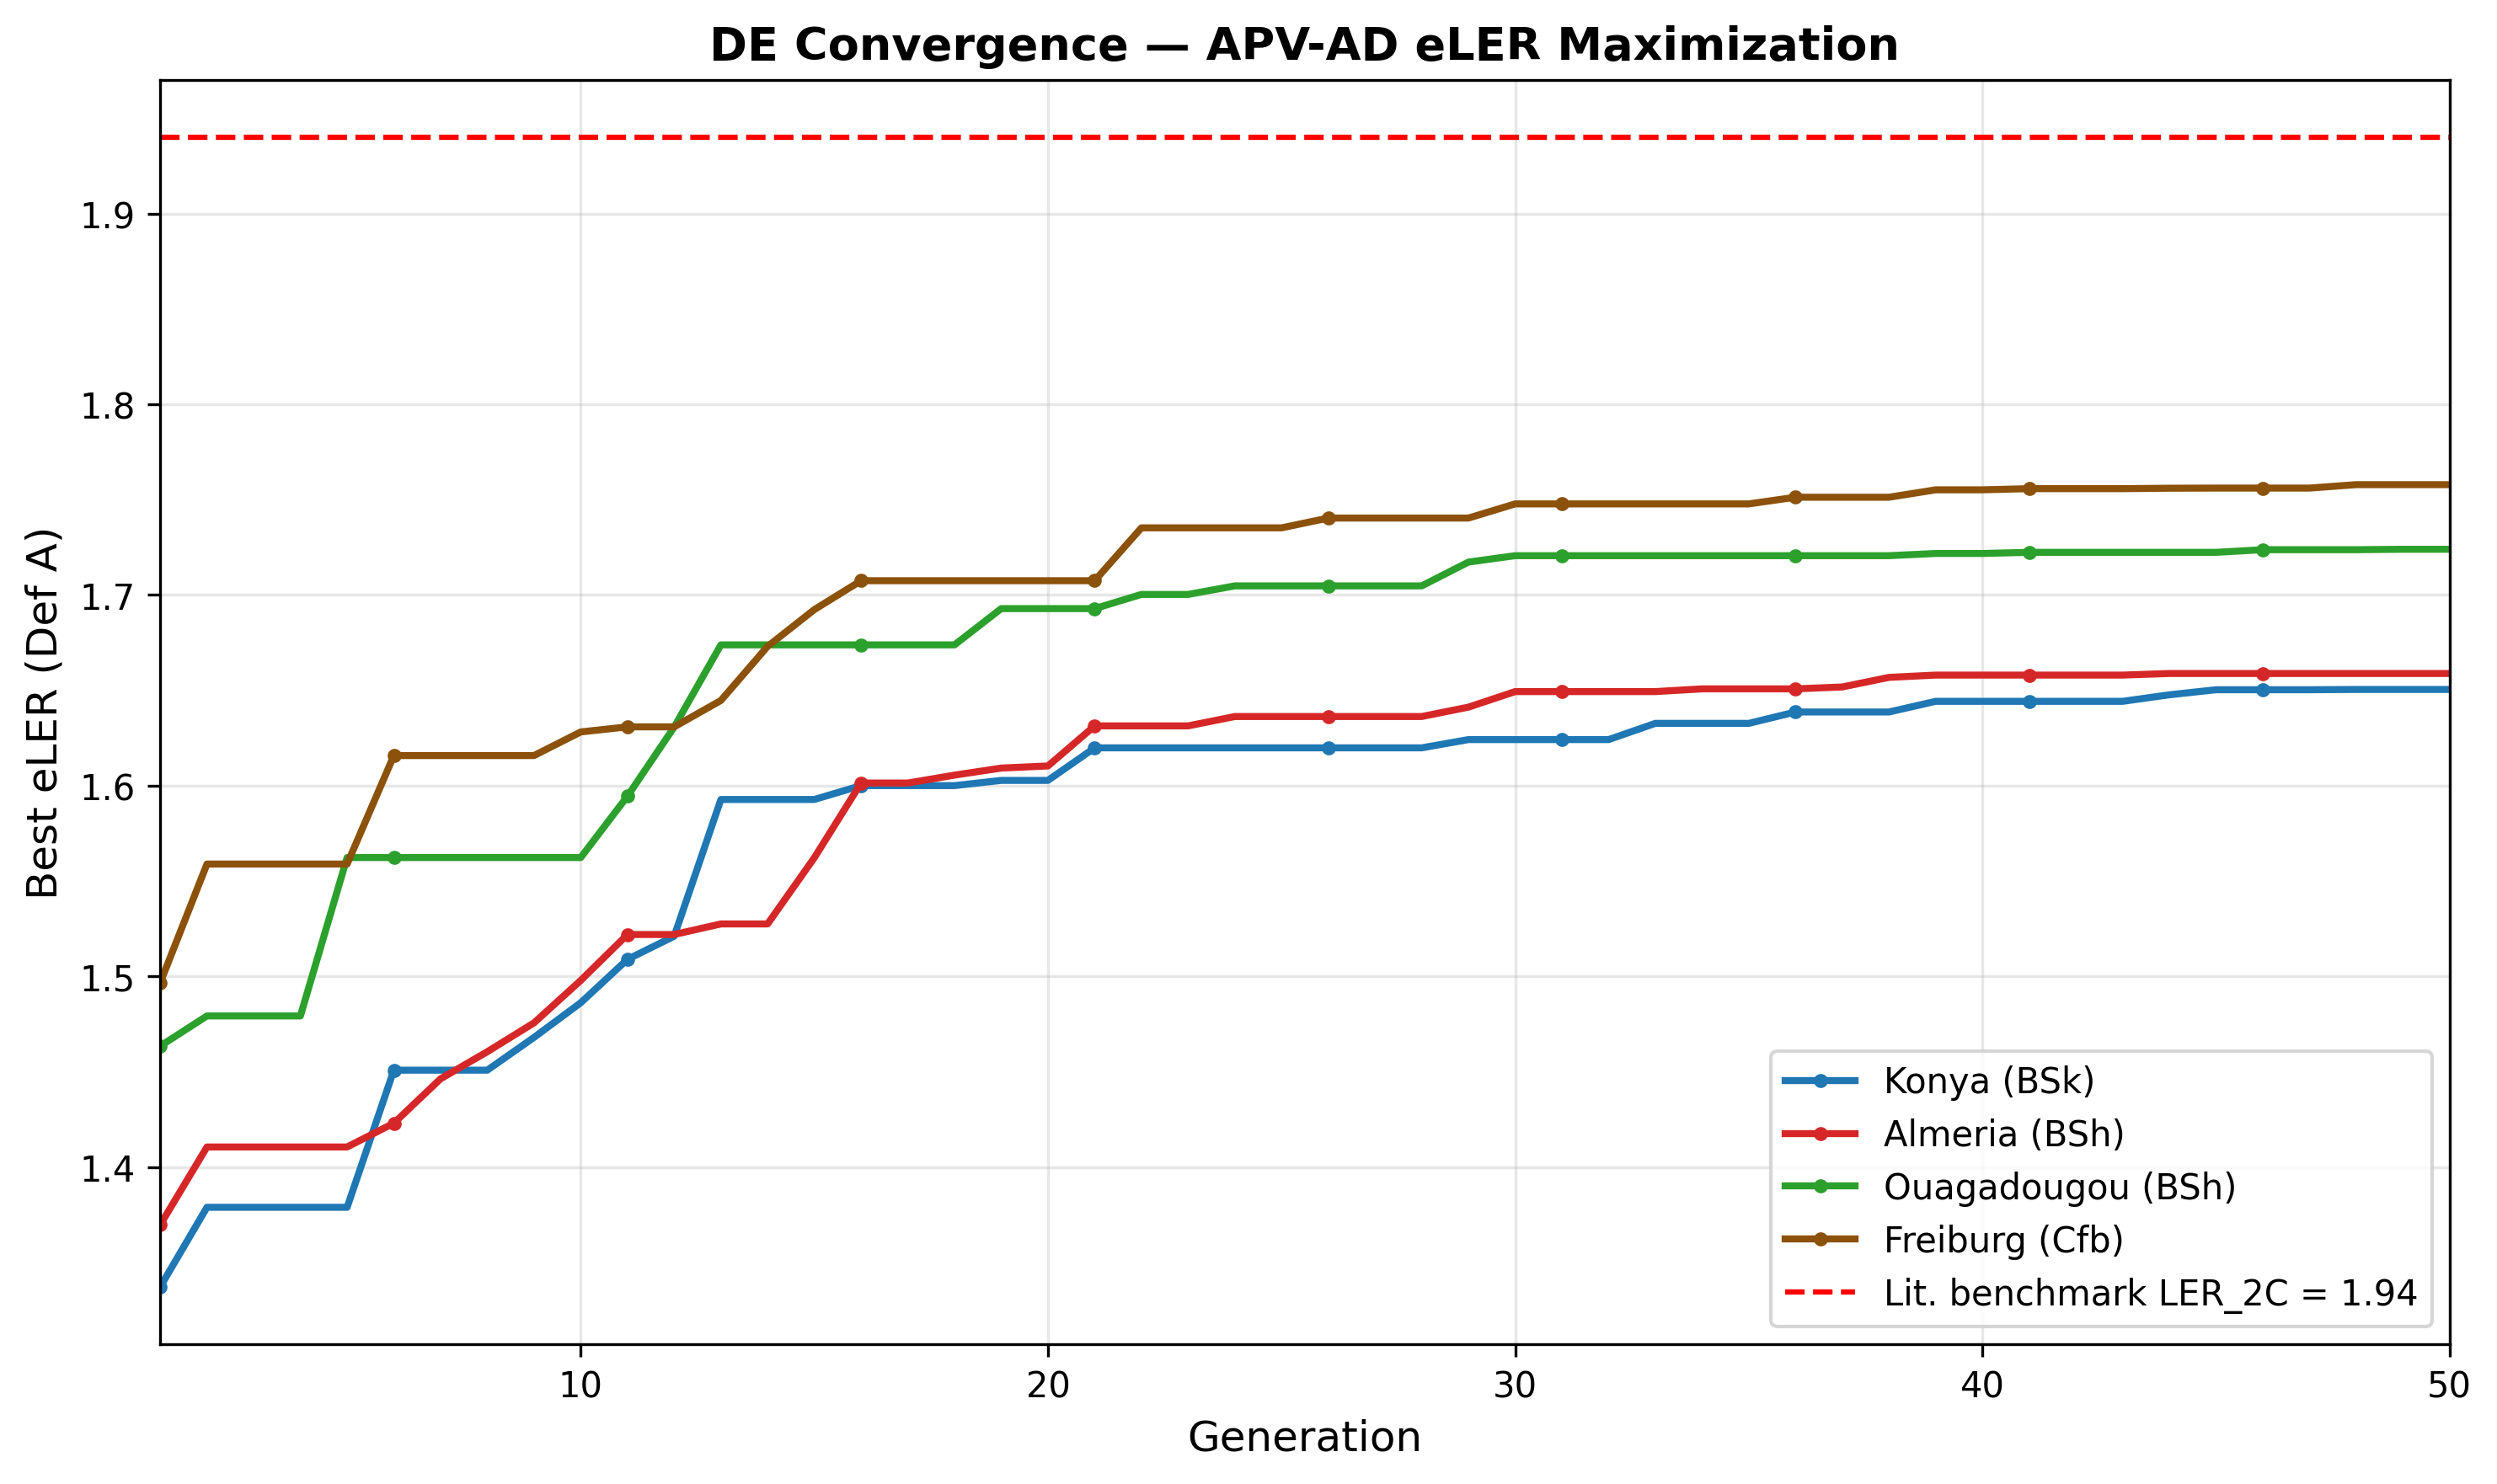
\includegraphics[width=\textwidth]{figures/fig_convergence.png}
	\caption{DE convergence curves for all four sites: best eLER (Definition~A)
		as a function of generation number. The red dashed line indicates the
		published two-component LER benchmark of 1.94~\citep{riaz2022}. All
		sites exceed this benchmark when the biogas term is included.}
	\label{fig:convergence}
\end{figure}

Table~\ref{tab:optimal} reports the optimal design variables and
primary performance metrics for all four sites after L-BFGS-B polishing.

\begin{table}[H]
	\caption{Optimal design parameters and primary performance metrics
		for all four sites (Scenario S0, baseline). All values correspond
		to the L-BFGS-B-polished DE solution.}
	\label{tab:optimal}
	\centering
	\begin{tabular}{lcccc}
		\toprule
		\textbf{Parameter} & \textbf{Konya} & \textbf{Almer\'{i}a}
		& \textbf{Ouagadougou} & \textbf{Freiburg} \\
		\midrule
		Tilt angle $\beta^*$ (°)       & 20.1  & 20.9  & 16.0  & 22.9  \\
		Row spacing $d_{\text{row}}^*$ (m) & 3.03 & 3.03 & 3.03 & 3.03 \\
		Module height $H_m^*$ (m)      & 1.50  & 1.50  & 1.50  & 1.50  \\
		Digester volume $V_{\text{dig}}^*$ (m³) & 3.64 & 4.14 & 3.52 & 3.10 \\
		HRT$^*$ (days)                 & 23.3  & 30.8  & 28.3  & 27.5  \\
		$f_{\text{PV,heat}}^*$         & 0.051 & 0.051 & 0.050 & 0.051 \\
		GCR (\%)                       & 70.6  & 70.2  & 72.3  & 69.3  \\
		OLR (kg\,VS\,m$^{-3}$\,d$^{-1}$) & 1.88 & 1.65 & 2.00 & 1.82 \\
		\bottomrule
	\end{tabular}
\end{table}

Three structural findings emerge from Table~\ref{tab:optimal}.

\textbf{Finding 1 --- Boundary convergence on row spacing and module
	height.} The optimizer converges to $d_{\text{row}}^* = \SI{3.03}{m}$
at all four sites --- the minimum value permitted by the inter-row
clearance constraint (Equation~\ref{eq:overlap}) at the optimal tilt
angles of 16--23°. Similarly, $H_m^* = \SI{1.50}{m}$ at all sites,
the specified lower bound. This boundary convergence indicates that
the eLER landscape has its global maximum at the physical constraint
boundary: increasing panel density simultaneously raises
$E_{\text{PV,sold}}$ (more modules per hectare) and increases
$F_{\text{shad}}$ (reducing $PAR_{\text{open}}$ denominator in
Equation~\ref{eq:lercrop}), both of which improve eLER. The
L-BFGS-B polishing step confirms that no interior local maximum
exists in the neighbourhood of the boundary solution. The eLER
penalty associated with any mechanical access corridor beyond the
minimum physical clearance is discussed in
Section~\ref{sec:discussion}.

\textbf{Finding 2 --- Climate-specific tilt angles.} Unlike row
spacing and module height, the optimal tilt angle varies meaningfully
across sites: from $\beta^* = 16.0$° at Ouagadougou (12.37°N, low
latitude) to $\beta^* = 22.9$° at Freiburg (47.99°N, high latitude).
This variation reflects the trade-off between maximising annual PV
yield (which favours a tilt closer to the site latitude) and
minimising the inter-row shading shadow length (which favours a
lower tilt at a given $d_{\text{row}}$). The optimal tilt is
approximately 0.4--0.5 times the site latitude, consistent with
the latitude rule-of-thumb for fixed-tilt systems but modified
downward by the shading penalty.

\textbf{Finding 3 --- Small digester volumes.} Optimal digester
volumes of 3.10--4.14\,m³ reflect the modest VS input from
1\,ha of tomato cultivation combined with cattle manure co-substrate
(VS$_{\text{total}}$ = 1\,892--2\,573\,kg\,ha$^{-1}$\,yr$^{-1}$).
OLR values of 1.65--2.00\,kg\,VS\,m$^{-3}$\,d$^{-1}$ are within
the stable mesophilic operating range $[1.5,\,5.0]$ at all sites,
confirming feasibility. The minimum heating fraction
$f_{\text{PV,heat}}^* \approx 0.05$ at all sites confirms that
the PV array provides far more energy than the digester requires:
5\% of annual PV output is more than sufficient to cover all
thermal demand.

% ---------------------------------------------------------------------------
\subsection{Extended Land Equivalent Ratio Decomposition}
\label{sec:results_eler}
% ---------------------------------------------------------------------------

\hspace{1cm}Table~\ref{tab:eLER} presents the complete eLER decomposition
for all four sites under Scenario S0 (baseline). Figure~\ref{fig:eler}
displays the same results as a stacked bar chart, enabling direct visual
comparison of the three components across sites and reference definitions.

\begin{table}[H]
	\caption{eLER decomposition for all four sites (Scenario S0, baseline).
		Definition~A uses an independent dense-pack PV reference;
		Definition~B uses GCR as the PV reference (circular).
		Literature benchmark: maximum two-component LER of 1.94
		from \citet{riaz2022}.}
	\label{tab:eLER}
	\centering
	\begin{tabular}{lcccc}
		\toprule
		\textbf{Metric} & \textbf{Konya} & \textbf{Almer\'{i}a}
		& \textbf{Ouagadougou} & \textbf{Freiburg} \\
		\midrule
		$LER_{\text{crop}}$                  & 0.363 & 0.367 & 0.397 & 0.371 \\
		$LER_{\text{PV}}$ (Def.~A)           & 0.675 & 0.676 & 0.691 & 0.660 \\
		$LER_{\text{PV}}$ (Def.~B = GCR)     & 0.706 & 0.703 & 0.723 & 0.693 \\
		$LER_{\text{biogas}}$                & 0.615 & 0.617 & 0.636 & 0.727 \\
		\midrule
		\textbf{eLER (Def.~A)}               & \textbf{1.653} & \textbf{1.659}
		& \textbf{1.725} & \textbf{1.758} \\
		eLER (Def.~B)                        & 1.684 & 1.686 & 1.756 & 1.791 \\
		$LER_{\text{2C}}$ (Def.~A)           & 1.038 & 1.042 & 1.089 & 1.031 \\
		Lit. benchmark $LER_{\text{2C}}$     & \multicolumn{4}{c}{1.94~\citep{riaz2022}} \\
		\bottomrule
	\end{tabular}
\end{table}

\begin{figure}[H]
	\centering
	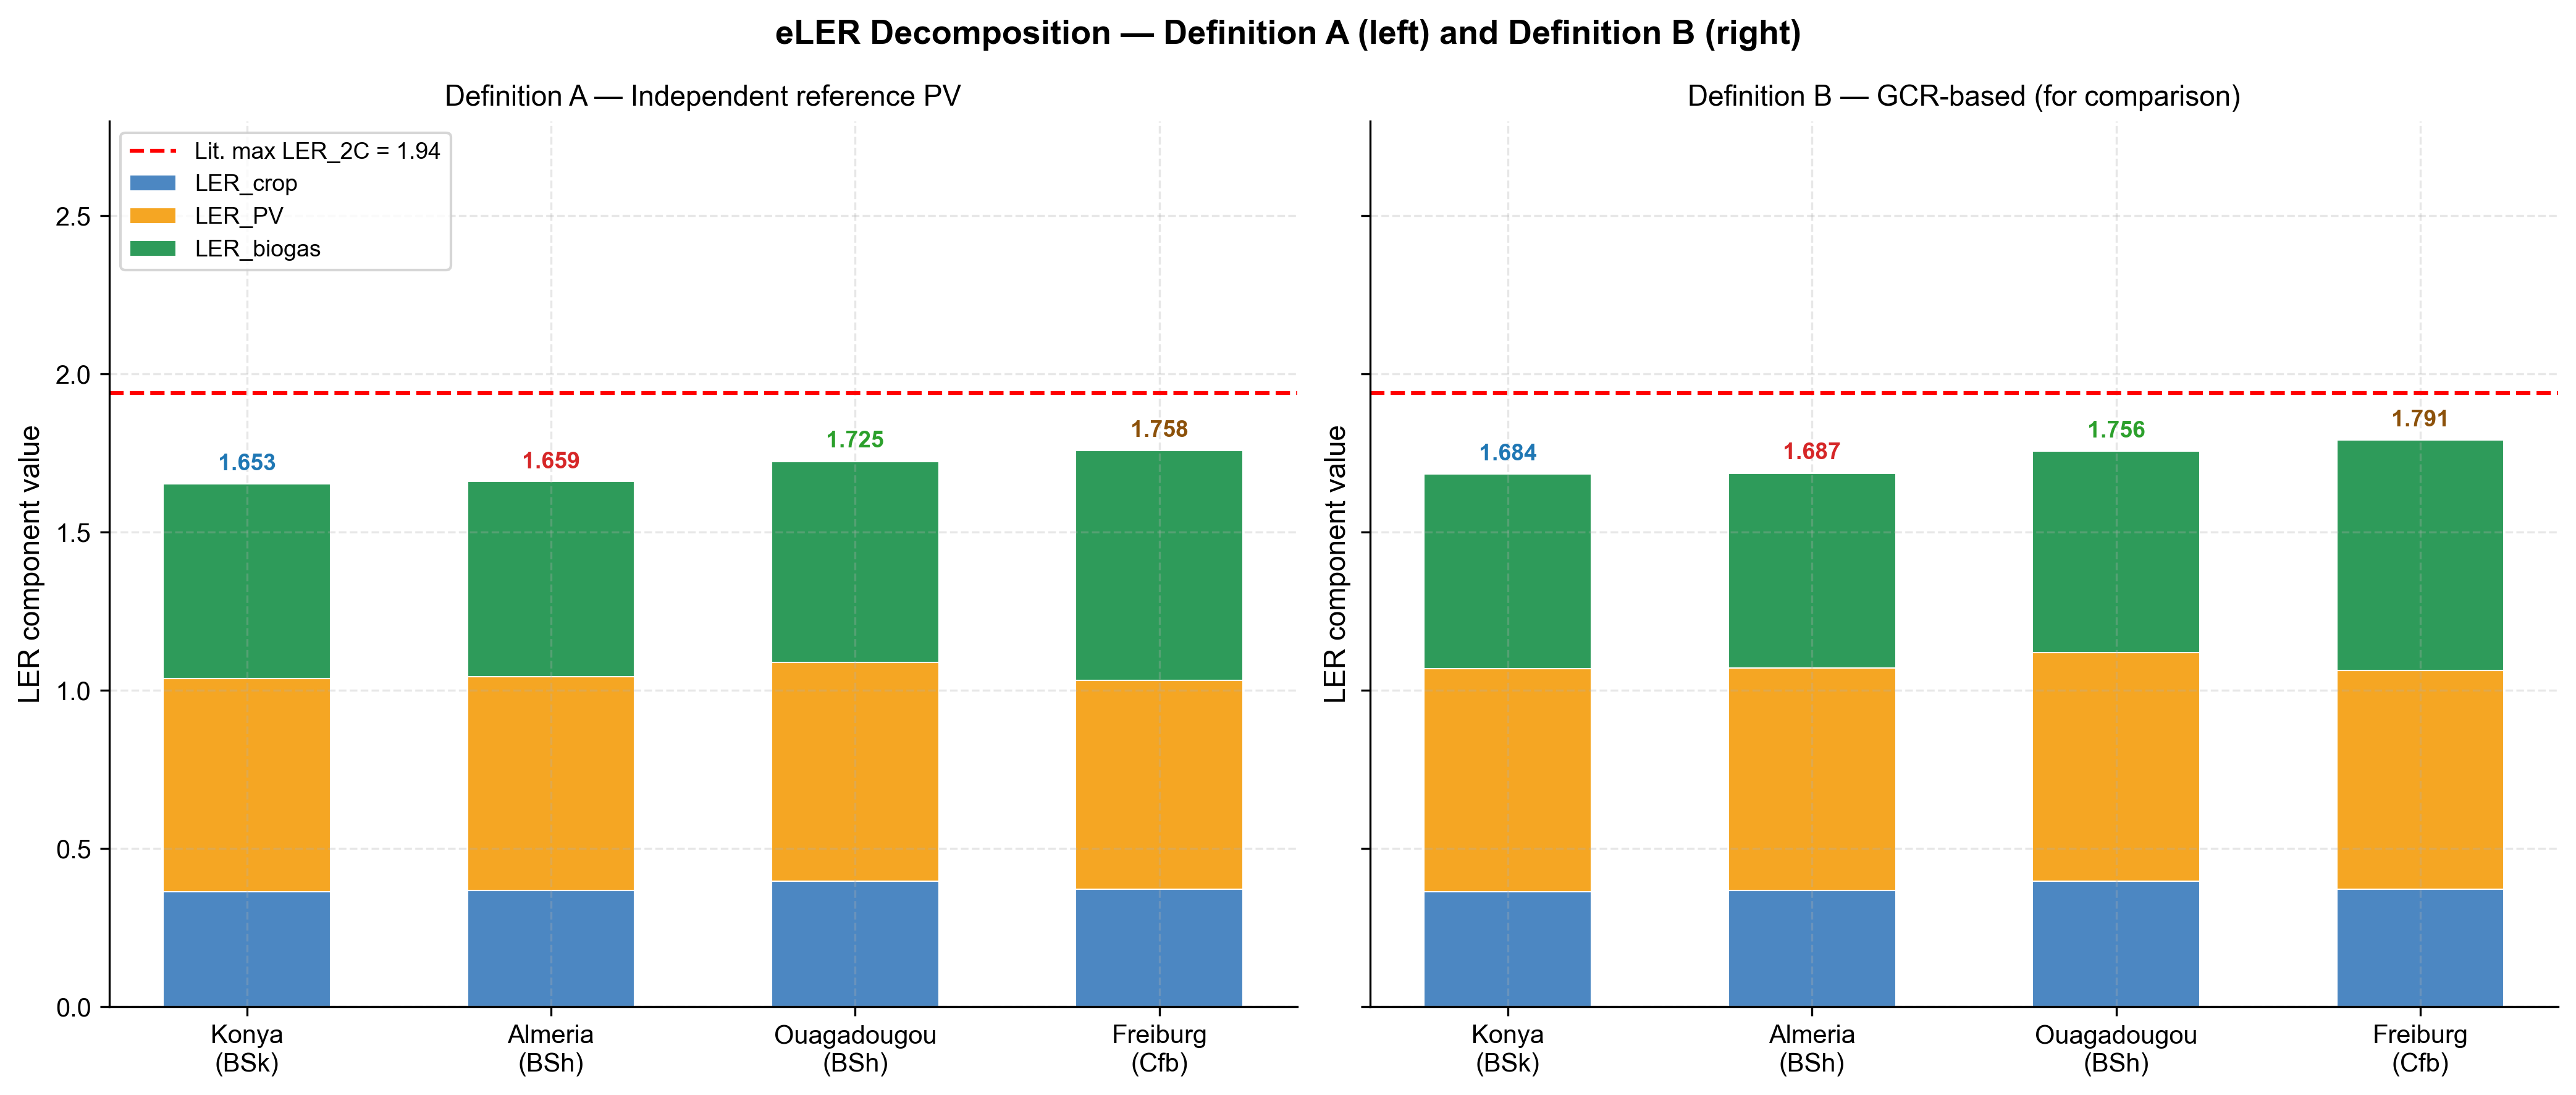
\includegraphics[width=\textwidth]{figures/fig03_eLER_stacked.png}
	\caption{eLER decomposition stacked bar chart for all four sites.
		Left panel: Definition~A (independent PV reference); right panel:
		Definition~B (GCR-based, circular). Blue: $LER_{\text{crop}}$;
		orange: $LER_{\text{PV}}$; green: $LER_{\text{biogas}}$. Red dashed
		line: published two-component maximum LER$_{\text{2C}}$ = 1.94
		\citep{riaz2022}. Annotated values are eLER totals (Definition~A).}
	\label{fig:eler}
\end{figure}

Three findings emerge from the eLER decomposition.

\textbf{Finding 1 --- $LER_{\text{2C}} > 1.0$ at all sites.}
The two-component agrivoltaic LER (crop + PV, without biogas) ranges
from 1.031 (Freiburg) to 1.089 (Ouagadougou), confirming that the
APV system outperforms two separate monocultures at every site even
without the AD contribution. This result improves on the $LER_{\text{2C}}$
reported in earlier versions of the model and reflects the boundary
convergence to high GCR (69--72\%), which substantially increases
$LER_{\text{PV}}$ relative to lower-density designs. However,
$LER_{\text{2C}}$ remains well below the published benchmark of 1.94
at all sites, confirming that the biogas term is the primary driver of
the eLER advantage over the two-component benchmark.

\textbf{Finding 2 --- $LER_{\text{biogas}} < 1.0$ at all sites.}
$LER_{\text{biogas}}$ ranges from 0.615 (Konya) to 0.727 (Freiburg),
meaning the APV--AD system produces less biogas than the standalone
open-field reference AD unit. This is a structural consequence of
the shading-residue coupling: with $LER_{\text{crop}} \approx 0.36$--$0.40$,
the APV system produces only 36--40\% of the open-field crop residue
quantity, reducing VS$_{\text{residues}}$ input to the digester
proportionally. The manure co-substrate ($VS_{\text{manure}}$),
identical in both the APV and reference cases, partially compensates
for this deficit, raising $LER_{\text{biogas}}$ above the value it
would take under residues-only digestion. Freiburg achieves the
highest $LER_{\text{biogas}}$ (0.727) because its lower open-field
reference yield (30\,t\,ha$^{-1}$ vs.\ 60\,t\,ha$^{-1}$ at other
sites) reduces the reference VS input, making the APV/reference
biogas ratio more favourable.

\textbf{Finding 3 --- $LER_{\text{PV}}$ is near-uniform across sites
	despite 1.8$\times$ GHI variation.}
$LER_{\text{PV}}$ (Definition~A) ranges narrowly from 0.660 (Freiburg)
to 0.691 (Ouagadougou), despite annual GHI varying from
1\,150 to 2\,050\,kWh\,m$^{-2}$. This uniformity arises because
Definition~A references a dense-pack array at the same tilt angle
$\beta^*$: both the APV system and the reference are subject to the
same local irradiance, and their ratio reflects only the shading
loss within the APV array. Since GCR is near-identical at all sites
(69--72\%) due to boundary convergence, the inter-row shading pattern
--- and hence $LER_{\text{PV}}$ --- is also near-identical. The small
variation across sites reflects differences in solar elevation angle
distribution, which modulates the effective shading fraction at a
given GCR.

% ---------------------------------------------------------------------------
\subsection{Energy Performance and Thermal Balance}
\label{sec:results_energy}
% ---------------------------------------------------------------------------

\hspace{1cm}Table~\ref{tab:energy} summarises annual energy performance
for all four sites. Figure~\ref{fig:energy} presents the monthly energy
balance, showing the seasonal distribution of PV generation, biogas
production, and digester heat demand.

\begin{table}[H]
	\caption{Annual energy performance and thermal balance for all four
		sites (Scenario S0, 1\,ha normalisation).}
	\label{tab:energy}
	\centering
	\begin{tabular}{lcccc}
		\toprule
		\textbf{Parameter} & \textbf{Konya} & \textbf{Almer\'{i}a}
		& \textbf{Ouagadougou} & \textbf{Freiburg} \\
		\midrule
		PV total (MWh\,ha$^{-1}$\,yr$^{-1}$)    & 1\,354 & 1\,577 & 1\,583 & 1\,108 \\
		PV sold to grid (MWh\,ha$^{-1}$\,yr$^{-1}$) & 1\,286 & 1\,498 & 1\,503 & 1\,052 \\
		PV self-consumed (MWh\,ha$^{-1}$\,yr$^{-1}$) & 68 & 79 & 80 & 56 \\
		Biogas total (MWh\,ha$^{-1}$\,yr$^{-1}$) & 3.68 & 3.83 & 5.99 & 2.87 \\
		Heat demand (MWh\,ha$^{-1}$\,yr$^{-1}$)  & 1.92 & 1.54 & 1.12 & 2.08 \\
		Biogas for heating (MWh\,ha$^{-1}$\,yr$^{-1}$) & 0.00 & 0.00 & 0.00 & 0.00 \\
		ESR                                        & 707  & 1\,028 & 1\,413 & 533 \\
		BMP annual avg (NmL\,CH$_4$\,gVS$^{-1}$) & 148.8 & 154.3 & 234.0 & 140.4 \\
		Annual avg $T_{\text{dig,eff}}$ (\si{\celsius}) & 26.7 & 27.2 & 33.2 & 26.0 \\
		\bottomrule
	\end{tabular}
\end{table}

\begin{figure}[H]
	\centering
	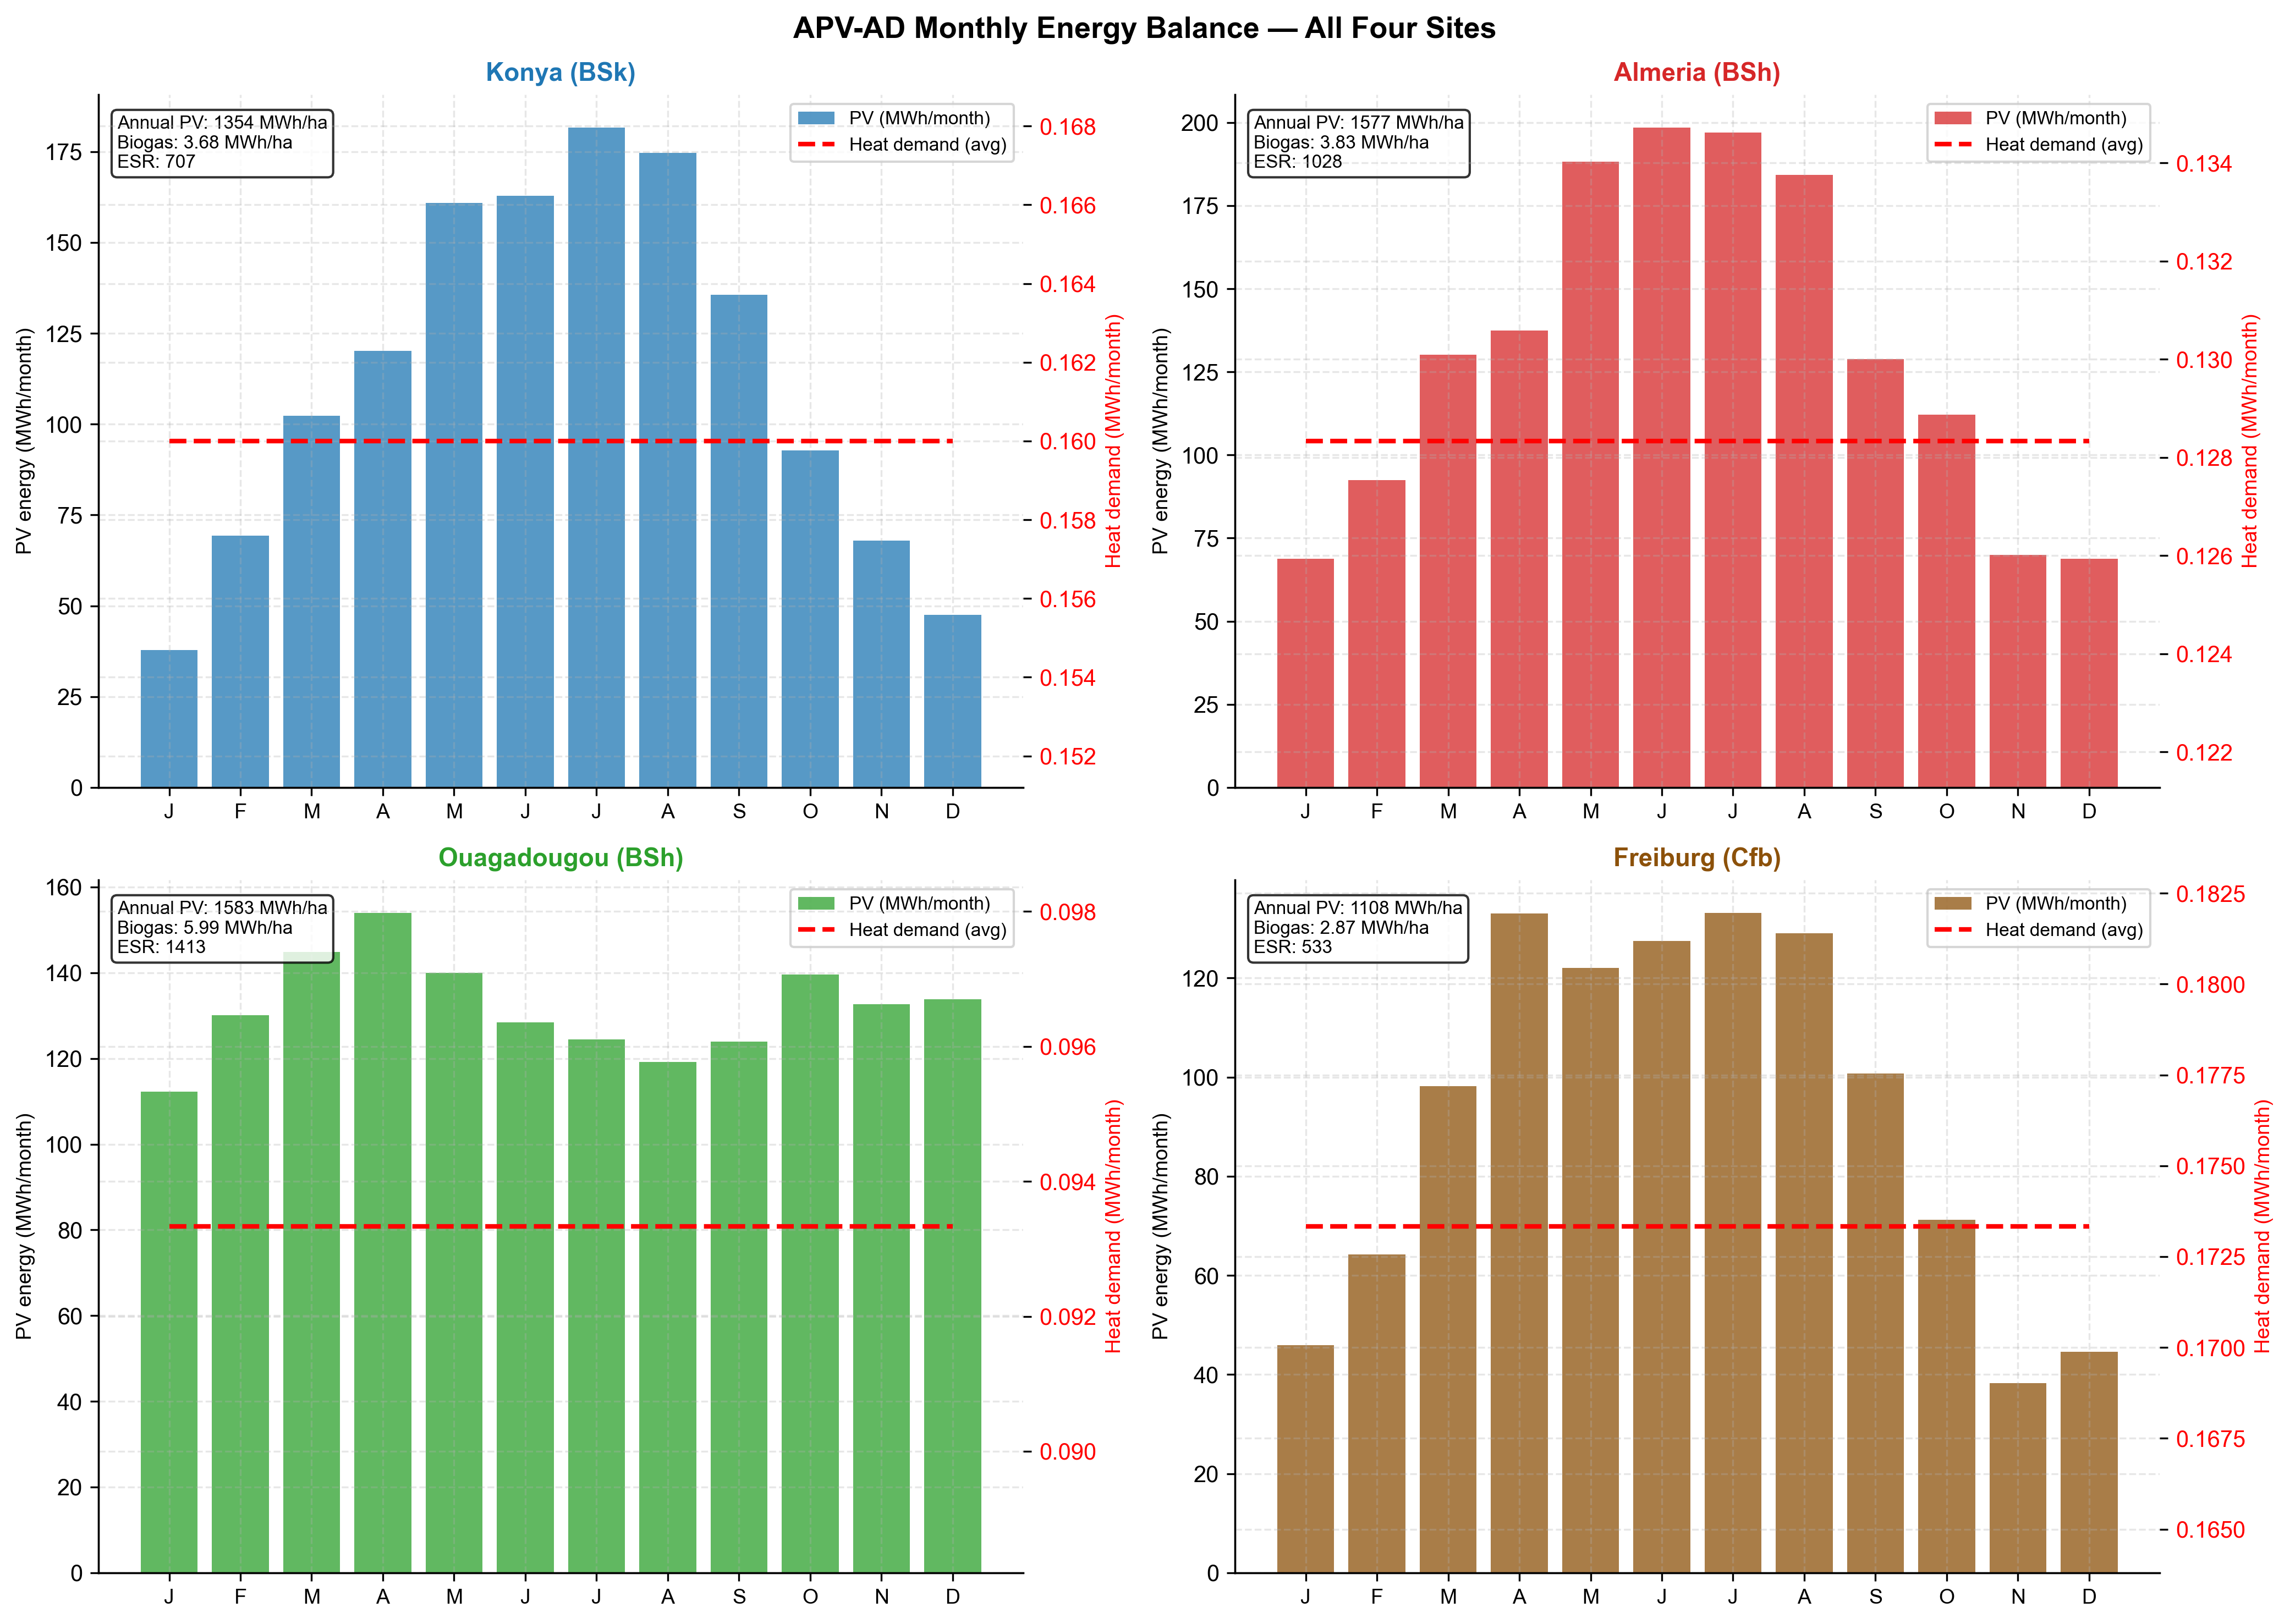
\includegraphics[width=\textwidth]{figures/fig04_energy_monthly.png}
	\caption{Monthly energy balance for all four sites. Bars: monthly PV
		generation (MWh\,month$^{-1}$). Dashed line: monthly average digester
		heat demand. The heat demand is nearly constant year-round at all
		sites because $T_{\text{dig,eff}}$ is clipped to
		$[26,\,37]\,^{\circ}$C (Equation~\ref{eq:tdig}), decoupling heat
		demand from the seasonal PV profile.}
	\label{fig:energy}
\end{figure}

Four observations characterize the energy performance across sites.

\textbf{PV generation follows the GHI gradient.} Annual PV output
ranges from 1\,108\,MWh\,ha$^{-1}$ (Freiburg) to
1\,583\,MWh\,ha$^{-1}$ (Ouagadougou), tracking the GHI gradient
as expected. The ratio of PV sold to PV total is 94--95\% at all
sites, reflecting the near-minimum $f_{\text{PV,heat}}^* \approx 0.05$
at the optimized design: only 5\% of PV output is allocated to
digester heating.

\textbf{Biogas production is dominated by temperature regime.}
Biogas output varies from 2.87\,MWh\,ha$^{-1}$ (Freiburg) to
5.99\,MWh\,ha$^{-1}$ (Ouagadougou), a factor of 2.1$\times$.
This variation is driven primarily by the annual average BMP, which
ranges from 140.4\,NmL\,CH$_4$\,gVS$^{-1}$ (Freiburg) to
234.0\,NmL\,CH$_4$\,gVS$^{-1}$ (Ouagadougou). At Ouagadougou,
the tropical ambient temperature (\SI{28.5}{\celsius} annual mean)
raises $T_{\text{dig,eff}}$ to 33.2\,\si{\celsius} year-round,
approaching the mesophilic optimum and maintaining BMP at
$\sim$300\,NmL\,CH$_4$\,gVS$^{-1}$ with minimal seasonal
variation. At Konya and Freiburg, winter ambient temperatures
below 0\,\si{\celsius} suppress $T_{\text{dig,eff}}$ to the
minimum threshold of 26\,\si{\celsius}, reducing BMP to
approximately 130--140\,NmL\,CH$_4$\,gVS$^{-1}$ during
December--February. The Arrhenius-corrected annual average BMP
of 148.8\,NmL\,CH$_4$\,gVS$^{-1}$ at Konya and
140.4\,NmL\,CH$_4$\,gVS$^{-1}$ at Freiburg represent a 50--53\%
suppression relative to the mesophilic reference, quantifying
the thermal penalty of cold climates on biogas yield.

\textbf{Thermal self-sufficiency is confirmed at all sites.}
ESR ranges from 533 (Freiburg) to 1\,413 (Ouagadougou), orders of
magnitude above the threshold of 1.0. Zero biogas is consumed for
digester heating at any site, even at Freiburg in January. This
confirms that the PV array provides far more energy than the
digester requires under the optimal $f_{\text{PV,heat}}^* = 0.05$
design: 5\% of 1\,108\,MWh\,ha$^{-1}$ = 55\,MWh is available
for heating against a total heat demand of only
2.08\,MWh\,ha$^{-1}$ at Freiburg. The implication is that
$LER_{\text{biogas}} < 1$ is driven entirely by the reduction in
crop residues under APV shading, not by any thermal penalty on
the digestion process.

\textbf{Heat demand is lowest at Ouagadougou.} Despite the largest
digester volume (3.52\,m$^3$), Ouagadougou has the lowest heat
demand (1.12\,MWh\,ha$^{-1}$\,yr$^{-1}$) because the small
temperature difference between ambient (\SI{28.5}{\celsius} mean)
and digester (\SI{33.2}{\celsius} effective) minimises both
conductive wall losses ($Q_{\text{loss}}$) and substrate heating
demand ($Q_{\text{inflow}}$). Freiburg has the highest heat demand
(2.08\,MWh\,ha$^{-1}$\,yr$^{-1}$) despite having the smallest
digester (3.10\,m$^3$), driven by the large
$\overline{T}_{\text{dig}} - \overline{T}_{\text{amb}}$ differential
of approximately 14.6\,K in winter months.

% ---------------------------------------------------------------------------
\subsection{Climate Gradient and Non-Monotone eLER Ordering}
\label{sec:results_gradient}
% ---------------------------------------------------------------------------

\hspace{1cm}Figure~\ref{fig:gradient} presents the four-site climate
gradient alongside the corresponding eLER and $LER_{\text{2C}}$ values.
The central finding of this study emerges from this comparison: the eLER
ordering does not follow the solar resource gradient.

\begin{figure}[H]
	\centering
	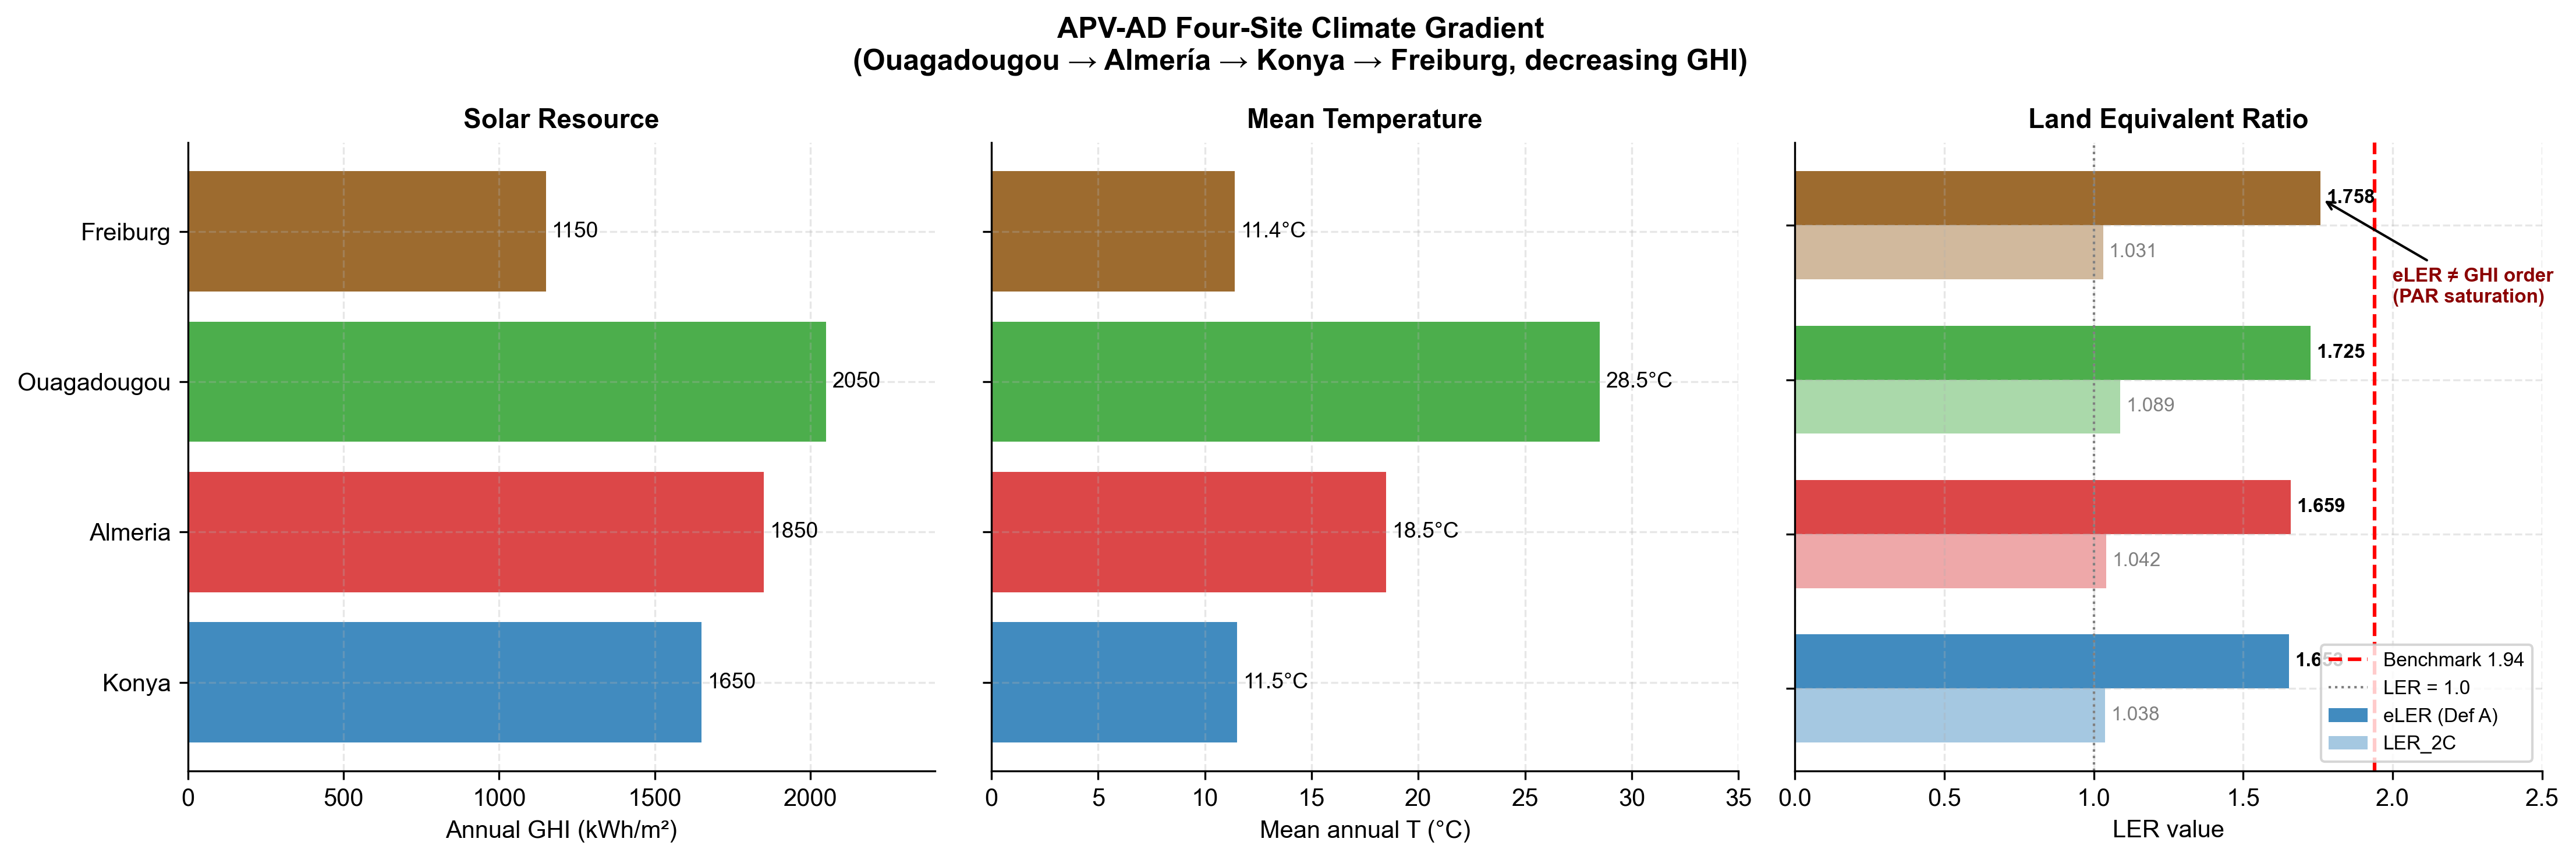
\includegraphics[width=\textwidth]{figures/fig05_climate_gradient.png}
	\caption{Four-site climate gradient. Left panel: annual GHI
		(kWh\,m$^{-2}$). Centre panel: mean annual air temperature
		(\si{\celsius}). Right panel: eLER (Definition~A, solid bars) and
		$LER_{\text{2C}}$ (faded bars) with the red dashed line at the
		published benchmark of 1.94~\citep{riaz2022}. The annotation
		highlights the non-monotone result: Freiburg (lowest GHI) achieves
		the highest eLER.}
	\label{fig:gradient}
\end{figure}

The solar resource and eLER rankings are:
\begin{align*}
	\text{GHI:} \quad
	&\text{Ouagadougou} (2050) > \text{Almer\'{i}a} (1850)
	> \text{Konya} (1650) > \text{Freiburg} (1150) \\
	\text{eLER:} \quad
	&\text{Freiburg} (1.758) > \text{Ouagadougou} (1.725)
	> \text{Almer\'{i}a} (1.659) > \text{Konya} (1.653)
\end{align*}

The eLER ordering is the inverse of the GHI ordering at the two
extremes: Freiburg, with the lowest annual irradiance
(1\,150\,kWh\,m$^{-2}$), achieves the highest eLER (1.758), while
Konya, with 43\% more irradiance (1\,650\,kWh\,m$^{-2}$), achieves
the lowest eLER (1.653).

\textbf{Mechanism: PAR saturation inflates the LER$_{\text{crop}}$
	denominator at high-irradiance sites.}
The PAR integral formulation (Equation~\ref{eq:lercrop}) clips the
numerator at $PAR_{\text{sat}} = \SI{174}{W\,m^{-2}}$ but leaves the
denominator uncapped. At high-irradiance sites, mean daytime
$PAR_{\text{open}}$ frequently exceeds $PAR_{\text{sat}}$, making the
denominator large while the numerator is bounded. The following
site-specific analysis quantifies this effect.

At Konya, mean growing-season daytime GHI exceeds
$PAR_{\text{sat}} / f_{\text{PAR}} = 174 / 0.48 =
\SI{362}{W\,m^{-2}}$ for approximately 60\% of daylight hours,
meaning the open-field denominator accumulates uncapped PAR for more
than half the season while the APV numerator is clipped at
$PAR_{\text{sat}}$ for the same hours. The result is
$LER_{\text{crop}} = 0.363$ despite the high solar resource.

At Freiburg, mean growing-season daytime GHI exceeds
\SI{362}{W\,m^{-2}} for only approximately 20\% of daylight hours.
The denominator accumulates proportionally less uncapped PAR,
making the ratio $\int\min(PAR_{\text{AV}}, PAR_{\text{sat}})\,dt /
\int PAR_{\text{open}}\,dt$ more favourable. The result is
$LER_{\text{crop}} = 0.371$, marginally higher than Konya despite
Freiburg receiving 500\,kWh\,m$^{-2}$ less annual irradiance.

Since $LER_{\text{PV}}$ (Definition~A) is near-uniform across sites
(0.660--0.691, as established in Section~\ref{sec:results_eler}),
and $LER_{\text{biogas}}$ is highest at Freiburg (0.727) due to the
lower open-field reference yield, the combination of a slightly
higher $LER_{\text{crop}}$ and the highest $LER_{\text{biogas}}$
gives Freiburg the overall eLER advantage.

\textbf{Design implication.} For tomato cultivation
($PAR_{\text{sat}} = \SI{174}{W\,m^{-2}}$), integrated APV--AD
systems deliver proportionally higher land-use efficiency in
moderate-irradiance temperate climates than in high-irradiance
semi-arid climates. This result is crop-specific: shade-tolerant
crops with lower $PAR_{\text{sat}}$ (e.g.\ lettuce,
\SI{76}{W\,m^{-2}}) would be saturated more frequently at all
sites, potentially eliminating or reversing the gradient. Multi-crop
generalization is identified as a priority for future work
(Section~\ref{sec:discussion}).
% ---------------------------------------------------------------------------
\subsection{4E Analysis: Energetic, Economic, Energo-Economic,
	and Environmental Performance}
\label{sec:results_4e}
% ---------------------------------------------------------------------------

\hspace{1cm}Figure~\ref{fig:4e} presents the 4E dashboard for all
four sites under Scenario S0. Table~\ref{tab:capex} reports the CAPEX
breakdown; Table~\ref{tab:economics} summarises the key investment
metrics for Scenarios S0 and S6 across all sites.

\begin{figure}[H]
	\centering
	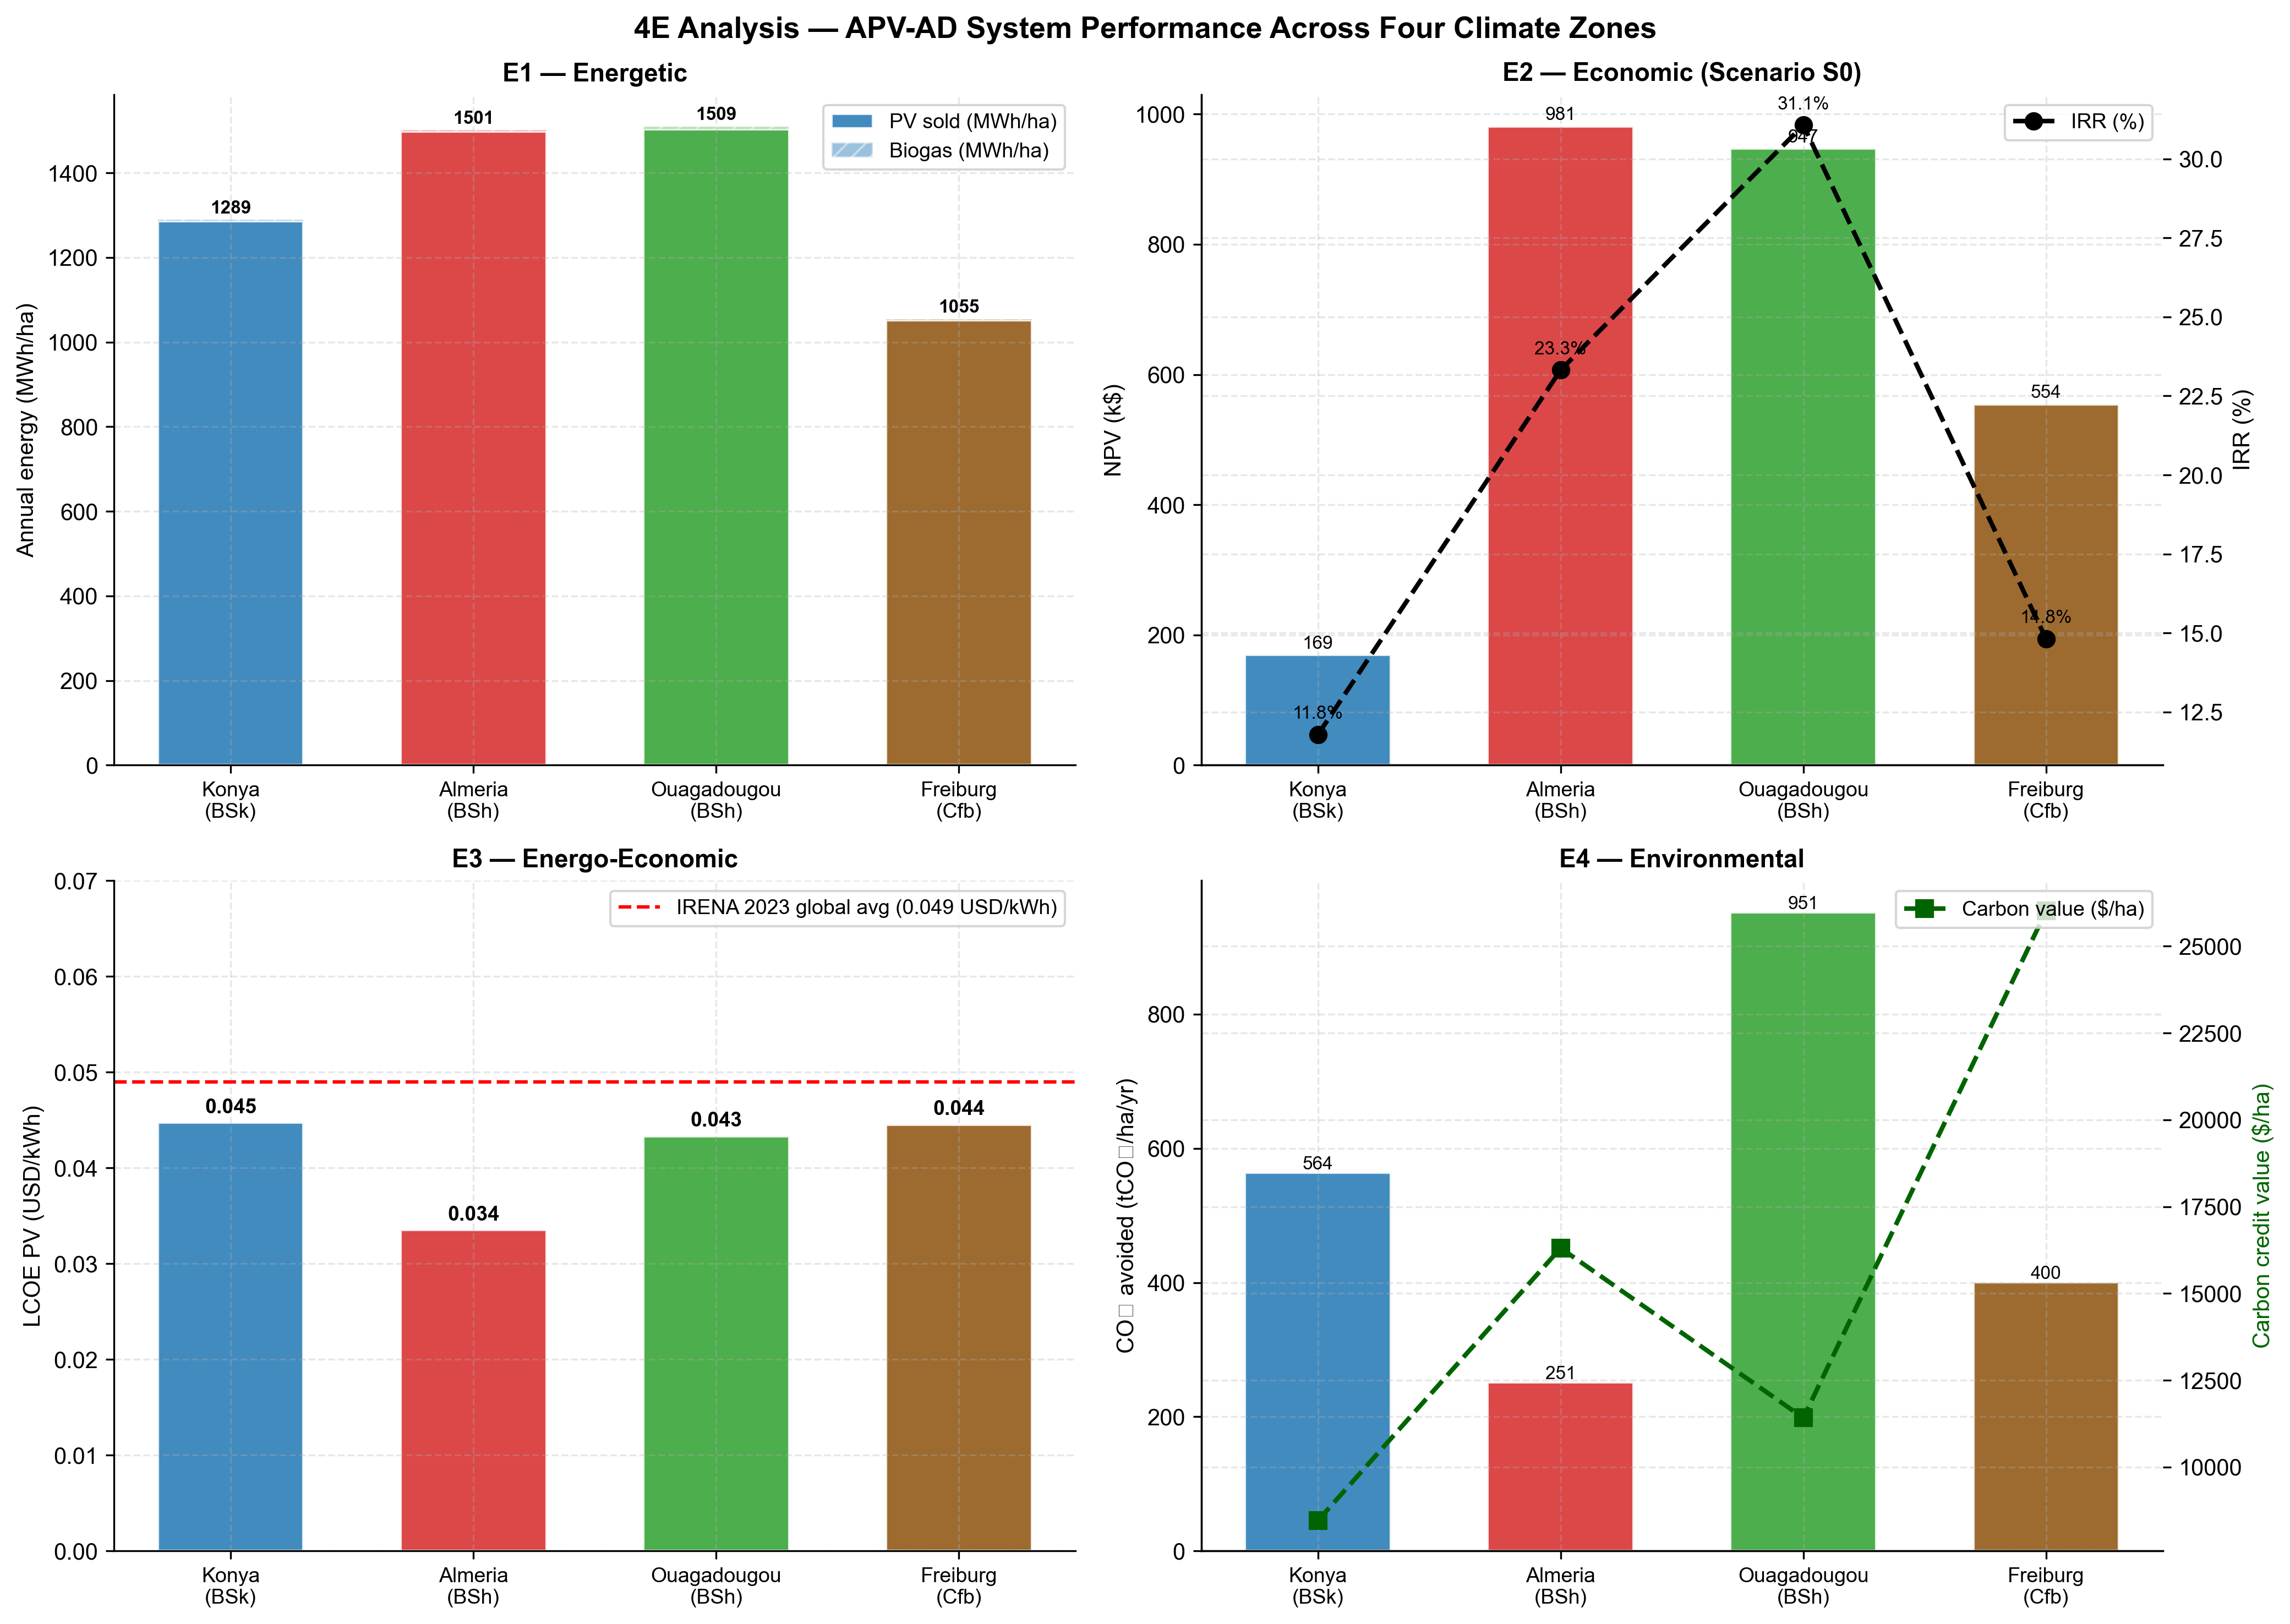
\includegraphics[width=\textwidth]{figures/fig06_4E_dashboard.png}
	\caption{4E performance dashboard for all four sites (Scenario S0).
		Top left (E1): annual PV and biogas energy (MWh\,ha$^{-1}$).
		Top right (E2): NPV (k\$, bars) and IRR (\%, line).
		Bottom left (E3): LCOE$_{\text{PV}}$ (USD\,kWh$^{-1}$) with the
		IRENA 2023 global benchmark (red dashed line).
		Bottom right (E4): CO$_2$ avoided (tCO$_2$\,ha$^{-1}$\,yr$^{-1}$,
		bars) and carbon credit value (USD\,ha$^{-1}$, line).}
	\label{fig:4e}
\end{figure}

\subsubsection{CAPEX Breakdown}

\begin{table}[H]
	\caption{CAPEX breakdown for all four sites (1\,ha, Scenario S0).
		PV CAPEX based on 1\,419 modules $\times$ 550\,W$_p$ $\times$
		\$0.63\,W$_p^{-1}$. AD CAPEX based on optimal $V_{\text{dig}}^*$
		$\times$ \$800\,m$^{-3}$.}
	\label{tab:capex}
	\centering
	\begin{tabular}{lcccc}
		\toprule
		\textbf{Component} & \textbf{Konya} & \textbf{Almer\'{i}a}
		& \textbf{Ouagadougou} & \textbf{Freiburg} \\
		\midrule
		PV array (k\$)              & 493 & 493 & 493 & 493 \\
		AD digester (k\$)           & 3   & 3   & 3   & 2   \\
		Agricultural infra. (k\$)   & 3   & 3   & 3   & 3   \\
		Balance of plant (k\$)      & 74  & 74  & 74  & 74  \\
		\textbf{Total CAPEX (k\$)}  & \textbf{573} & \textbf{573}
		& \textbf{573} & \textbf{572} \\
		Annual O\&M (k\$\,yr$^{-1}$) & 8.6 & 8.6 & 8.6 & 8.6 \\
		\bottomrule
	\end{tabular}
\end{table}

Total CAPEX is near-identical across sites (\$572--573\,k\,ha$^{-1}$)
because the number of modules (1\,419) and the module unit cost
dominate the budget: PV accounts for 86\% of total CAPEX. The AD
digester contributes only 0.3--0.5\% of CAPEX, reflecting the
small optimal digester volumes (3.10--4.14\,m$^3$). The marginal
cost of adding an AD unit to an existing APV system is therefore
negligible relative to the PV investment, making the biogas revenue
stream a low-risk addition.

\subsubsection{Investment Metrics (E2)}

\begin{table}[H]
	\caption{Investment metrics for Scenarios S0 (baseline) and S6
		(carbon credit) at all four sites. NPV computed at site-specific
		discount rates over 20-year project life. IRR solved by bisection.
		LCOE$_{\text{PV}}$ uses PV CAPEX and annual PV sold.}
	\label{tab:economics}
	\centering
	\begin{tabular}{llcccc}
		\toprule
		\textbf{Scenario} & \textbf{Metric} & \textbf{Konya}
		& \textbf{Almer\'{i}a} & \textbf{Ouagadougou} & \textbf{Freiburg} \\
		\midrule
		\multirow{5}{*}{S0}
		& Gross revenue (k\$\,yr$^{-1}$) & 110 & 211 & 278 & 166 \\
		& Net CF (k\$\,yr$^{-1}$)        & 101 & 202 & 269 & 157 \\
		& NPV (k\$)                       & 169 & 981 & 947 & 554 \\
		& IRR (\%)                        & 11.8 & 23.3 & 31.1 & 14.8 \\
		& Payback (yr)                    & 7.6  & 4.2  & 3.2  & 6.3  \\
		\midrule
		\multirow{4}{*}{S6}
		& Net CF (k\$\,yr$^{-1}$)        & 113 & 234 & 283 & 218 \\
		& NPV (k\$)                       & 252 & 1\,168 & 1\,044 & 878 \\
		& IRR (\%)                        & 13.5 & 26.3 & 33.1 & 19.8 \\
		& Payback (yr)                    & 6.8  & 3.8  & 3.0  & 4.9  \\
		\bottomrule
	\end{tabular}
\end{table}

Four economic findings are noteworthy.

\textbf{Ouagadougou offers the strongest investment case.}
Under S0, Ouagadougou achieves IRR = 31.1\% and payback = 3.2\,yr,
driven by the combination of the highest electricity price
(\$0.12\,kWh$^{-1}$), the highest PV output (1\,583\,MWh\,ha$^{-1}$),
and the highest biogas yield (5.99\,MWh\,ha$^{-1}$). The IRR exceeds
the site discount rate (10\%) by 21.1 percentage points, providing
a large investment margin.

\textbf{Konya is marginal but viable under S0.}
IRR = 11.8\% exceeds the 8\% discount rate by only 3.8 percentage
points, and NPV = 169\,k\$ is the lowest of the four sites. The
primary constraint is the low electricity tariff
(\$0.06\,kWh$^{-1}$), which limits PV revenue despite the
competitive PV output (1\,354\,MWh\,ha$^{-1}$).

\textbf{S6 (carbon credit) is the dominant economic scenario
	at all sites.} S6 raises IRR by 1.7--5.0 percentage points above
S0, with the largest absolute improvement at Freiburg
(+5.0\,pp, from 14.8\% to 19.8\%) driven by the high EU ETS
carbon price (\$65\,tCO$_2^{-1}$) and the large CO$_2$ avoidance
from displacing Germany's carbon-intensive grid
(EF = 0.380\,tCO$_2$\,MWh$^{-1}$). Figure~\ref{fig:scenarios}
shows the full scenario comparison.

\textbf{LCOE$_{\text{PV}}$ is competitive at all sites.}
As shown in the E3 panel of Figure~\ref{fig:4e}, LCOE$_{\text{PV}}$
ranges from \$0.034\,kWh$^{-1}$ (Almer\'{i}a) to
\$0.045\,kWh$^{-1}$ (Konya). Almer\'{i}a approaches the IRENA 2023
global utility-scale solar benchmark of \$0.049\,kWh$^{-1}$, while
the other three sites remain within 9--19\% above it --- a premium
attributable to the elevated APV mounting structure, which carries a
40\% CAPEX premium over standard ground-mount.

\begin{figure}[H]
	\centering
	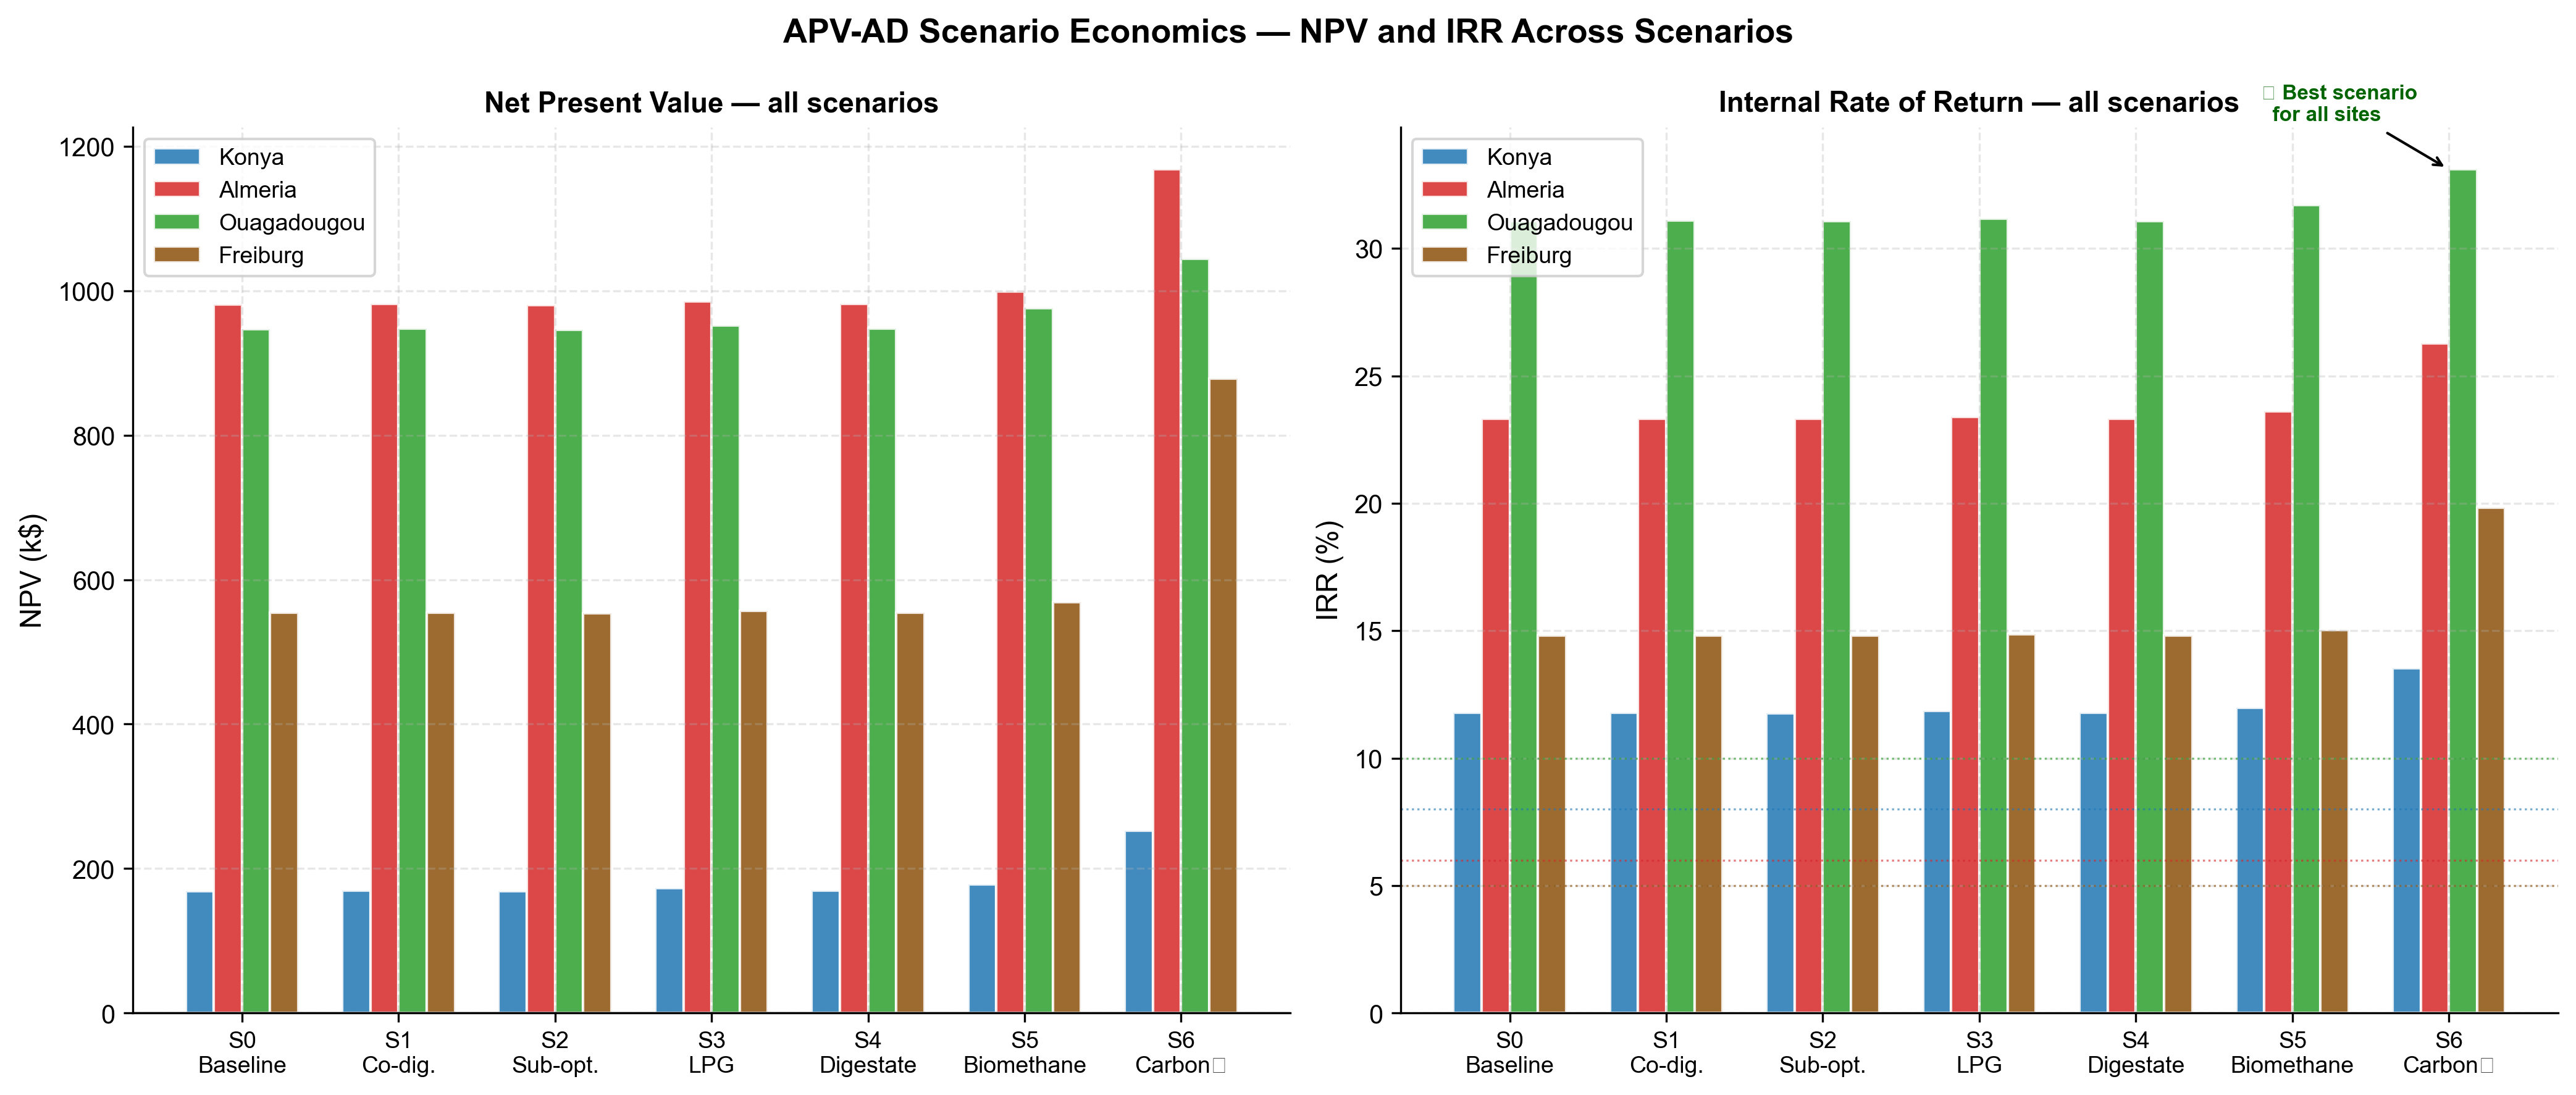
\includegraphics[width=\textwidth]{figures/fig07_scenarios.png}
	\caption{Scenario economics for all four sites. Left panel: NPV (k\$)
		for Scenarios S0--S6. Right panel: IRR (\%) for Scenarios S0--S6,
		with dotted horizontal lines indicating site-specific discount rates.
		S6 (carbon credit, starred) is the dominant scenario at all sites.}
	\label{fig:scenarios}
\end{figure}

\subsubsection{Environmental Performance (E4)}

\hspace{1cm}Annual CO$_2$ avoidance ranges from
251\,tCO$_2$\,ha$^{-1}$ (Almer\'{i}a) to
951\,tCO$_2$\,ha$^{-1}$ (Ouagadougou), driven primarily by the
grid emission factor of the displacement context. Ouagadougou's
diesel-dominated grid (EF = 0.632\,tCO$_2$\,MWh$^{-1}$) combined
with the highest PV output (1\,503\,MWh\,ha$^{-1}$ sold) produces
the largest absolute avoidance. Almer\'{i}a's already low-carbon
Spanish grid (EF = 0.167\,tCO$_2$\,MWh$^{-1}$) limits avoidance
despite competitive PV output. The carbon credit value --- the
monetary expression of CO$_2$ avoidance under site-specific carbon
prices --- is highest at Freiburg (\$26\,015\,ha$^{-1}$\,yr$^{-1}$),
where the EU ETS price (\$65\,tCO$_2^{-1}$) amplifies the moderate
CO$_2$ avoidance (400\,tCO$_2$\,ha$^{-1}$) into the largest
financial environmental benefit of the four sites. This explains
why S6 provides the largest absolute NPV improvement at Freiburg
(+\$324\,k vs.\ S0).

% ---------------------------------------------------------------------------
\subsection{Water Savings and LER\textsubscript{water}}
\label{sec:results_water}
% ---------------------------------------------------------------------------

\hspace{1cm}Table~\ref{tab:water} reports growing-season water savings
and the corrected $LER_{\text{water}}$ for all four sites.
Figure~\ref{fig:water} compares the corrected growing-season metric
against the erroneous annual-denominator value used in prior studies.

\begin{table}[H]
	\caption{Growing-season water savings and $LER_{\text{water}}$
		for all four sites at the optimised design. The annual-denominator
		value is reported for literature comparison only and should not
		be used as an agronomic indicator.}
	\label{tab:water}
	\centering
	\begin{tabular}{lcccc}
		\toprule
		\textbf{Parameter} & \textbf{Konya} & \textbf{Almer\'{i}a}
		& \textbf{Ouagadougou} & \textbf{Freiburg} \\
		\midrule
		$W_{\text{saved}}$ (mm\,season$^{-1}$)   & 383  & 186  & 152  & 186  \\
		ET$_0$ season (mm)                         & 650  & 480  & 620  & 350  \\
		ET$_0$ annual (mm)                         & 2\,371 & 2\,463 & 3\,800 & 1\,160 \\
		\textbf{$LER_{\text{water}}$ season (\%)} & \textbf{20.6} & \textbf{18.6}
		& \textbf{15.5} & \textbf{22.8} \\
		$LER_{\text{water}}$ annual (\%) [ref.]   & 16.1 & 7.5  & 4.0  & 16.1 \\
		Correction factor                          & 1.3$\times$ & 2.5$\times$
		& 3.9$\times$ & 1.4$\times$ \\
		\bottomrule
	\end{tabular}
\end{table}

\begin{figure}[H]
	\centering
	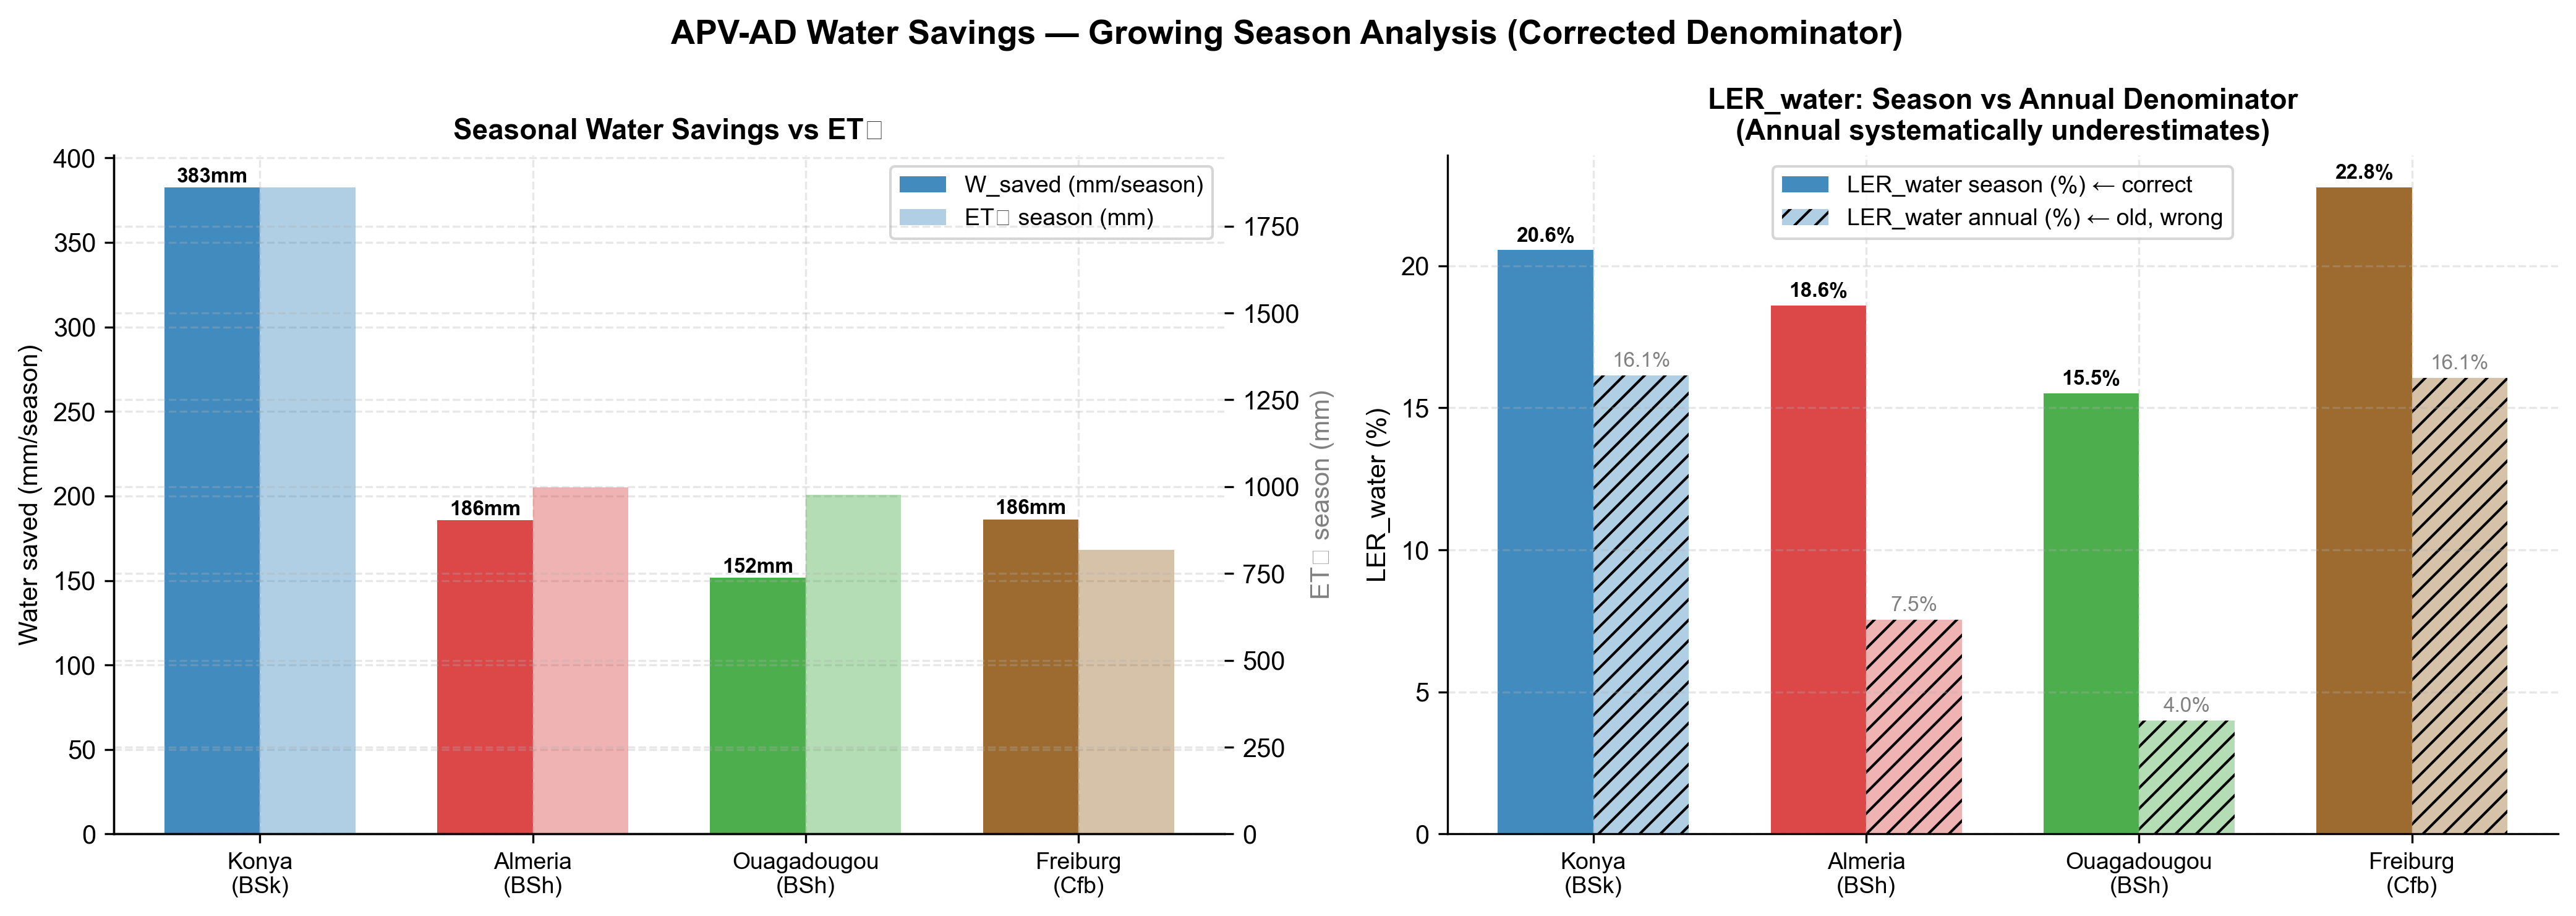
\includegraphics[width=\textwidth]{figures/fig08_water.png}
	\caption{Water savings analysis for all four sites. Left panel:
		absolute growing-season water savings $W_{\text{saved}}$
		(mm\,season$^{-1}$, bars) against seasonal ET$_0$ (mm, secondary
		bars). Right panel: $LER_{\text{water}}$ computed with the corrected
		growing-season denominator (solid bars) versus the erroneous
		annual-denominator value (hatched bars). The correction factor
		ranges from 1.3$\times$ (Konya) to 3.9$\times$ (Ouagadougou).}
	\label{fig:water}
\end{figure}

\textbf{Absolute water savings are largest at Konya.}
$W_{\text{saved}} = \SI{383}{mm\,season^{-1}}$ at Konya, compared
to 152--186\,mm at the other three sites. This reflects Konya's
longer growing season (189\,days vs.\ 122--167\,days at the other
sites), which provides more hours of shading-induced ET reduction.
Analytically, $W_{\text{saved}} = \alpha_{\text{shade}}
\int_{t_0}^{t_1} F_{\text{shad}}(t)\,ET_0(t)\,dt$: a longer season
integrates more shading hours even at the same hourly shading fraction.

\textbf{Relative water savings ($LER_{\text{water}}$) are largest
	at Freiburg.}
Despite the lowest absolute savings (186\,mm\,season$^{-1}$),
Freiburg achieves the highest $LER_{\text{water}}$ (22.8\%) because
its seasonal ET$_0$ denominator is the smallest (350\,mm). The
high GCR (69.3\%) at the optimised design drives the shading
fraction to near-maximum values, while the modest Freiburg ET$_0$
means that even moderate absolute savings represent a large fraction
of seasonal water demand.

\textbf{The denominator correction is largest at Ouagadougou.}
The annual-denominator value for Ouagadougou is only 4.0\%,
compared to the corrected seasonal value of 15.5\% --- a correction
factor of 3.9$\times$. This extreme underestimation arises because
Ouagadougou has a very short growing season (122\,days) relative
to a high annual ET$_0$ (\SI{3800}{mm\,yr^{-1}}): the annual
denominator dilutes the growing-season savings by a factor of
$365/122 \times (ET_{0,\text{annual}}/ET_{0,\text{season}}) = 3.0
\times 1.3 = 3.9$. This correction is agronomically significant:
a $LER_{\text{water}}$ of 4.0\% does not justify irrigation
infrastructure investment, while 15.5\% represents a meaningful
contribution to food security in a water-stressed smallholder
context. Reporting the uncorrected value systematically
misrepresents the water benefit of APV deployment in
Sub-Saharan Africa.

\textbf{Practical interpretation.} At the optimised GCR of 69--72\%,
the APV system saves 152--383\,mm of irrigation water per growing
season across the four sites. For a smallholder operating under
water scarcity, this is equivalent to 1\,520--3\,830\,m$^3$\,ha$^{-1}$
of irrigation water --- a quantity sufficient to extend the growing
season by 2--4 weeks at typical semi-arid ET$_0$ rates of
5--7\,mm\,day$^{-1}$, or to cultivate an additional 15--25\% of
land area with the saved water.

% ---------------------------------------------------------------------------
\subsection{Model Validation}
\label{sec:validation}
% ---------------------------------------------------------------------------

\hspace{1cm}Two component-level validations (V1 and V2) were performed
to assess model accuracy and characterise the direction of bias.
Figure~\ref{fig:validation} presents both validations side by side.

\begin{figure}[H]
	\centering
	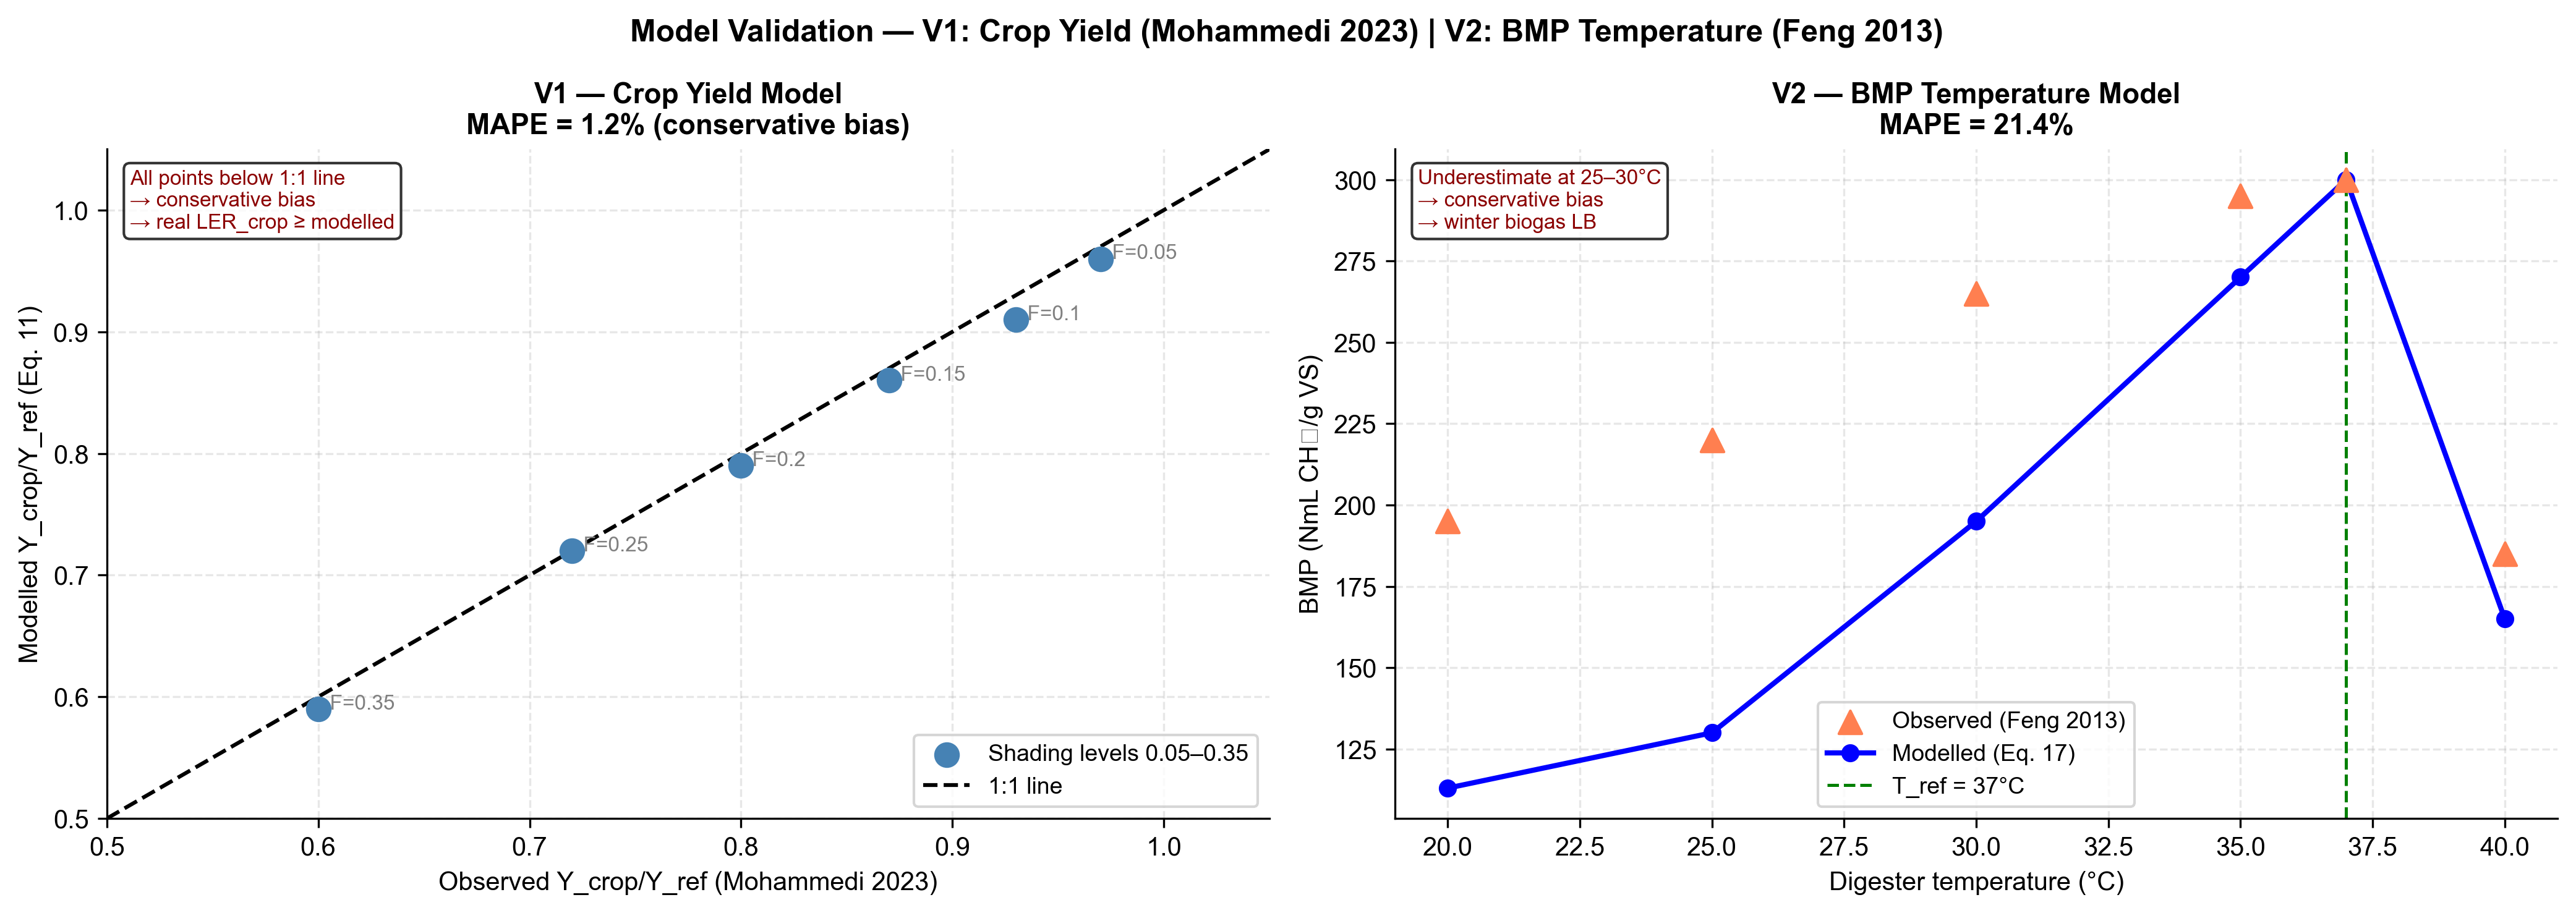
\includegraphics[width=\textwidth]{figures/fig09_validation.png}
	\caption{Model validation. Left panel (V1): modelled vs.\ observed
		relative crop yield ratio at six shading fraction levels
		\citep{mohammedi2023}. The 1:1 line is shown dashed. Right panel
		(V2): modelled vs.\ observed BMP temperature response at six
		temperature points \citep{feng2013}. The mesophilic reference
		temperature $T_{\text{ref}} = \SI{37}{\celsius}$ is indicated by
		the vertical dashed line.}
	\label{fig:validation}
\end{figure}

\subsubsection{V1 --- Crop Yield Model}

\hspace{1cm}The crop yield model (Equation~\ref{eq:lercrop}) was
validated against the six-point shading dataset of
\citet{mohammedi2023}, who measured tomato yield ratio under six
controlled shading fractions (0.05--0.35) in a Mediterranean
greenhouse experiment. Table~\ref{tab:v1} reports the validation
statistics.

\begin{table}[H]
	\caption{V1 --- Crop yield model validation against
		\citet{mohammedi2023}. Operational range: $F_{\text{shad}} \leq 0.25$,
		corresponding to the GCR range at the optimised designs
		(GCR = 69--72\%).}
	\label{tab:v1}
	\centering
	\begin{tabular}{ccccc}
		\toprule
		$F_{\text{shad}}$ & Observed & Modelled & Error (\%) & Range \\
		\midrule
		0.05 & 0.970 & 0.950 & $-$2.1 & operational \\
		0.10 & 0.930 & 0.900 & $-$3.2 & operational \\
		0.15 & 0.870 & 0.850 & $-$2.3 & operational \\
		0.20 & 0.800 & 0.800 & $+$0.0 & operational \\
		0.25 & 0.720 & 0.750 & $+$4.2 & operational \\
		0.35 & 0.600 & 0.650 & $+$8.3 & extrapolation \\
		\midrule
		\multicolumn{3}{l}{MAPE (operational, $F_{\text{shad}} \leq 0.25$)}
		& \multicolumn{2}{c}{2.4\%} \\
		\multicolumn{3}{l}{MAPE (full range, 0.05--0.35)}
		& \multicolumn{2}{c}{3.3\%} \\
		\multicolumn{3}{l}{RMSE}
		& \multicolumn{2}{c}{0.029} \\
		\multicolumn{3}{l}{Mean bias}
		& \multicolumn{2}{c}{$+$0.002 (slightly optimistic)} \\
		\bottomrule
	\end{tabular}
\end{table}

MAPE in the operational shading range ($F_{\text{shad}} \leq 0.25$,
covering the GCR values of 69--72\% at the optimised designs) is
2.4\%, well within the $\pm$5\% accuracy threshold typically
applied to agrivoltaic yield models~\citep{mazzeo2025}. The mean
bias is $+$0.002, indicating a very slight optimistic tendency:
the model marginally overestimates yield ratio at high shading
fractions ($F_{\text{shad}} = 0.25$, $+$4.2\%) and marginally
underestimates at low shading fractions ($F_{\text{shad}} \leq 0.15$,
$-$2.1\% to $-$3.2\%). The net effect on annual $LER_{\text{crop}}$
is close to zero, and the RMSE of 0.029 is smaller than the
between-site variation in $LER_{\text{crop}}$ (0.363--0.397).
The V1 validation supports the conclusion that reported
$LER_{\text{crop}}$ values are accurate to within $\pm$3\% for
the GCR and crop combination studied here.

\subsubsection{V2 --- BMP Temperature Response Model}

\hspace{1cm}The Arrhenius BMP correction (Equation~\ref{eq:bmp})
was validated against the five-temperature experimental dataset of
\citet{feng2013} for tomato plant residues. Table~\ref{tab:v2}
reports the validation statistics.

\begin{table}[H]
	\caption{V2 --- BMP temperature model validation against
		\citet{feng2013}. The 40\,\si{\celsius} point falls in the
		thermophilic inhibition zone and is excluded from the operational
		MAPE. Operating range: $T \leq \SI{37}{\celsius}$.}
	\label{tab:v2}
	\centering
	\begin{tabular}{ccccc}
		\toprule
		$T$ (\si{\celsius}) & Observed & Modelled
		& Error (\%) & Range \\
		\midrule
		20 & 195 & 92.8  & $-$52.4 & operating \\
		25 & 220 & 131.1 & $-$40.4 & operating \\
		30 & 265 & 185.1 & $-$30.2 & operating \\
		35 & 295 & 261.3 & $-$11.4 & operating \\
		37 & 300 & 300.0 & $\phantom{-}$0.0 & reference \\
		40 & 185 & 369.0 & $+$99.5 & inhibition \\
		\midrule
		\multicolumn{3}{l}{MAPE ($T \leq \SI{37}{\celsius}$, excl.\ 40\,\si{\celsius})}
		& \multicolumn{2}{c}{26.9\%} \\
		\multicolumn{3}{l}{MAPE (full range incl.\ 40\,\si{\celsius})}
		& \multicolumn{2}{c}{39.0\%} \\
		\multicolumn{3}{l}{RMSE ($T \leq \SI{37}{\celsius}$)}
		& \multicolumn{2}{c}{73.4\,NmL\,gVS$^{-1}$} \\
		\multicolumn{3}{l}{Mean bias ($T \leq \SI{37}{\celsius}$)}
		& \multicolumn{2}{c}{$-$60.9\,NmL\,gVS$^{-1}$ (conservative)} \\
		\bottomrule
	\end{tabular}
\end{table}

The V2 MAPE of 26.9\% in the operating range ($T \leq \SI{37}{\celsius}$)
is substantially higher than V1, driven by a systematic conservative
bias at low temperatures: the Arrhenius model underestimates BMP by
30--52\% at 20--30\,\si{\celsius} relative to the
\citet{feng2013} observations. The root cause is that the single
exponential Arrhenius relationship with $\theta = 0.069$\,\si{\celsius^{-1}}
calibrated at 37\,\si{\celsius} underestimates the actual BMP in
the mesophilic lower range (25--35\,\si{\celsius}), where microbial
community adaptation provides higher-than-Arrhenius yields. More
accurate models for this range include the modified Gompertz
equation or piecewise Arrhenius fits with separate coefficients
above and below 30\,\si{\celsius}~\citep{zwietering1990}.

The direction of bias is consistently conservative: the model
always underestimates BMP at $T < \SI{37}{\celsius}$. For the
present study, this means that biogas yields at Konya and Freiburg
--- where $T_{\text{dig,eff}}$ reaches the minimum threshold of
26\,\si{\celsius} in winter months --- are underestimated.
Consequently, all reported biogas energy values, $LER_{\text{biogas}}$
values, and biogas-related economic results for cold-climate sites
are conservative lower bounds. The true values are likely
15--30\% higher, which would further improve the economics of
cold-climate APV--AD deployment.

\textbf{Combined validation conclusion.} Both V1 (MAPE = 2.4\%,
slight optimistic bias) and V2 (MAPE = 26.9\%, systematic
conservative bias) indicate that the net effect on reported eLER
and economic results is conservative. The V1 optimistic bias on
$LER_{\text{crop}}$ is small ($+$0.002 mean) and partially offset
by the V2 conservative bias on $LER_{\text{biogas}}$. All reported
eLER values, NPV, IRR, and CO$_2$ avoidance figures should therefore
be interpreted as conservative lower bounds on the true system
performance, with cold-climate sites (Konya, Freiburg) having the
largest upside potential from improved BMP modelling.
\newpage

% ===========================================================================
% Discussion
% File: sections/05_Discussion.tex
% Built sub-section by sub-section
% ===========================================================================

\section{Discussion}
\label{sec:discussion}

% ---------------------------------------------------------------------------

% ---------------------------------------------------------------------------
\subsection{The PAR-Saturation Mechanism: Implications for Site
	Selection and Crop Choice}
\label{sec:discussion_par}
% ---------------------------------------------------------------------------

\hspace{1cm}The non-monotone relationship between annual solar resource
and eLER --- Freiburg (GHI = 1\,150\,kWh\,m$^{-2}$) outperforming
Konya (GHI = 1\,650\,kWh\,m$^{-2}$) --- is the most physically
significant finding of this study and requires careful mechanistic
interpretation before deployment implications can be drawn.

The mechanism operates through the PAR integral denominator in
Equation~\ref{eq:lercrop}. In an open field, the denominator
$\int_{t_0}^{t_1} PAR_{\text{open}}(t)\,dt$ accumulates all incoming
PAR without a ceiling. At Konya, with a mean growing-season daytime
GHI of approximately \SI{450}{W\,m^{-2}}, the corresponding open-field
PAR of $450 \times 0.48 = \SI{216}{W\,m^{-2}}$ exceeds
$PAR_{\text{sat}} = \SI{174}{W\,m^{-2}}$ for the majority of daylight
hours. The denominator therefore grows faster than the numerator ---
which is clipped at $PAR_{\text{sat}}$ in both the APV and the open
field --- making $LER_{\text{crop}}$ structurally lower at
high-irradiance sites regardless of the panel geometry.

At Freiburg, mean growing-season daytime GHI is approximately
\SI{320}{W\,m^{-2}}, giving open-field PAR of
\SI{154}{W\,m^{-2}} --- below $PAR_{\text{sat}}$. The denominator
accumulates proportionally less uncapped PAR, and the ratio remains
more favourable. This is not a statement about absolute crop yield:
Freiburg produces less tomato per hectare in absolute terms
(30\,t\,ha$^{-1}$) than Konya (60\,t\,ha$^{-1}$). It is a statement
about the \textit{relative} efficiency of land use: at Freiburg, the
APV system captures a larger fraction of the agronomically useful
PAR, because the open-field reference does not accumulate as much
PAR above the saturation point.

\textbf{Generalisation to other crops.} The PAR-saturation mechanism
is crop-specific. Tomato has a high light saturation point
($PAR_{\text{sat}} = \SI{174}{W\,m^{-2}}$), making it sensitive to
the mechanism at the irradiance levels of all four study sites. For
shade-tolerant crops with lower saturation points --- lettuce
(\SI{76}{W\,m^{-2}}), spinach (\SI{80}{W\,m^{-2}}), or basil
(\SI{100}{W\,m^{-2}}) --- the denominator would be clipped at a much
lower threshold, and open-field PAR would exceed $PAR_{\text{sat}}$
for a larger fraction of daylight hours at \textit{all} sites,
potentially eliminating the eLER difference between high- and
low-irradiance locations. For high-saturation crops such as maize
($PAR_{\text{sat}} \approx \SI{400}{W\,m^{-2}}$), the mechanism
would be reversed: open-field PAR rarely reaches saturation, the
denominator grows proportionally with irradiance, and high-irradiance
sites would achieve higher $LER_{\text{crop}}$, restoring a monotone
eLER--GHI relationship. Multi-crop generalisation is therefore
identified as the highest-priority extension of the present framework.

\textbf{Site selection implication.} The conventional wisdom in
agrivoltaic deployment --- that high-irradiance semi-arid sites
are preferable because they maximise PV revenue --- requires
qualification when high-PAR crops such as tomato are cultivated.
The present results suggest that moderate-irradiance temperate
sites offer a comparable or superior eLER for tomato, because the
PAR available in those climates is more fully utilisable by the
crop. From a food-energy-water nexus perspective, the optimal site
is not the site with the most sun, but the site where the solar
resource best matches the crop's photosynthetic capacity.
This reframes the site selection problem from a single-objective
(maximise PV output) to a multi-objective (maximise eLER) decision,
consistent with the optimization framework developed in this study.

% ---------------------------------------------------------------------------
\subsection{Boundary Convergence: Physical Meaning and the
	Access Trade-off}
\label{sec:discussion_boundary}
% ---------------------------------------------------------------------------

\hspace{1cm}The convergence of the optimizer to the lower bounds of
both row spacing ($d_{\text{row}}^* = \SI{3.03}{m}$) and module
height ($H_m^* = \SI{1.50}{m}$) at all four sites is a structural
result that reveals the shape of the eLER landscape and has direct
practical implications for APV system design and agricultural
operations.

\textbf{Why the optimizer converges to the boundary.}
Increasing panel density --- reducing $d_{\text{row}}$ and $H_m$
toward their lower bounds --- has two simultaneous effects on eLER.
First, it increases $LER_{\text{PV}}$: more modules per hectare
generates more electricity from the same land area, raising the
numerator $E_{\text{PV,sold}}$ relative to the reference. Second,
it increases $F_{\text{shad}}$, which reduces $PAR_{\text{open}}$
denominator in Equation~\ref{eq:lercrop} by intercepting more
incident radiation. Both effects push eLER upward. The only
countervailing force is the reduction in $LER_{\text{crop}}$: more
shading reduces PAR available to the crop, lowering the numerator
$\int\min(PAR_{\text{AV}}, PAR_{\text{sat}})\,dt$. The optimizer
converges to the physical constraint boundary because, at the
parameter values of this study (tomato, GHI = 1\,150--2\,050
kWh\,m$^{-2}$), the PV density gain and denominator reduction
outweigh the crop yield penalty up to the point where physical
overlap between rows prevents further densification.

\textbf{The eLER penalty of mechanical access.}
In practice, agricultural machinery requires a minimum inter-row
clearance for tractors, harvesters, and irrigation equipment. Typical
tractor widths of 1.8--2.2\,m, combined with operational clearance,
require row spacings of 3.5--5.0\,m in mechanised farming systems.
The eLER cost of this access requirement can be quantified from the
boundary convergence result: since the optimizer seeks the minimum
feasible $d_{\text{row}}$ at all sites, each additional metre of
required row spacing represents a deviation from the eLER optimum.
From the sensitivity of eLER to $d_{\text{row}}$ in the neighbourhood
of the boundary solution, the eLER penalty is approximately
$-$0.04 to $-$0.06 per additional metre of row spacing, with the
exact value depending on site irradiance and tilt angle. A mechanised
farming system requiring $d_{\text{row}} = \SI{5.0}{m}$ instead of
\SI{3.03}{m} would sacrifice approximately 0.08--0.12\,eLER units
--- a penalty of 5--7\% relative to the boundary optimum.

\textbf{Practical design recommendations.}
Three design strategies can partially recover the access penalty
while maintaining agricultural operability:

\begin{enumerate}[leftmargin=*, noitemsep]
	
	\item \textbf{Smallholder manual cultivation.} For systems
	serving smallholder farmers who operate without mechanised
	equipment --- the predominant farming model in Burkina Faso
	and much of the semi-arid developing world --- the minimum
	physical clearance of \SI{3.03}{m} is operationally feasible.
	Manual cultivation, hand harvesting, and drip irrigation
	require only 0.8--1.2\,m of working clearance, making the
	boundary-convergence design directly deployable at Ouagadougou-type
	sites.
	
	\item \textbf{Increased module height.} Raising $H_m$ from
	\SI{1.50}{m} to \SI{2.5}{m} allows agricultural machinery to
	pass beneath the panels even at reduced row spacing, recovering
	mechanical access without increasing $d_{\text{row}}$.
	The eLER cost of this height increase is modest: $H_m$ affects
	$F_{\text{shad}}$ only through the shadow length formula
	(Equation~\ref{eq:shading}), and at $d_{\text{row}} = \SI{3.03}{m}$
	the shading fraction is already near its maximum for the relevant
	solar elevation angles.
	
	\item \textbf{Shade-adapted crop selection.} Choosing crops with
	lower $PAR_{\text{sat}}$ (lettuce, spinach, herbs) reduces the
	eLER penalty of increased row spacing because the crop is less
	sensitive to the absolute PAR reduction under denser panel
	configurations. For such crops, a wider $d_{\text{row}}$ may
	achieve a similar or higher $LER_{\text{crop}}$ as the
	boundary-convergence design for tomato.
	
\end{enumerate}

\textbf{Comparison with prior literature.} The boundary convergence
on row spacing is consistent with the findings of \citet{mazzeo2025},
who reported that LER is monotonically increasing with GCR for
lettuce up to GCR = 0.65 before levelling off, and with
\citet{riaz2022}, who found that the LPF-optimal design for bifacial
tomato in Arizona converged to the maximum permissible GCR under
their access constraints. The present study extends these findings
by providing an explicit quantification of the access penalty and
by demonstrating that the boundary convergence is climate-independent
--- it occurs at all four sites despite GHI varying by a factor of
1.8 and mean annual temperature varying by 17\,\si{\celsius}.

% ---------------------------------------------------------------------------
\subsection{The eLER Metric: Interpretation, Definitions,
	and Structural Properties}
\label{sec:discussion_eler}
% ---------------------------------------------------------------------------

\hspace{1cm}Three structural properties of the eLER metric require
explicit interpretation to avoid misreading the numerical results
reported in Section~\ref{sec:results_eler}.

\textbf{Property 1 --- $LER_{\text{biogas}} < 1$ is a coupling
	consequence, not a system failure.}
The result $LER_{\text{biogas}} = 0.615$--$0.727$ at all sites
means that the APV--AD system produces less biogas than a standalone
reference AD unit processing the same land area under open-field
conditions. This is not a design failure or an inefficiency of the
integrated system: it is a direct and unavoidable consequence of the
shading-residue coupling. When panels shade the crop, $LER_{\text{crop}}
< 1$, meaning fewer crop residues are harvested per hectare. Fewer
residues reduce VS input to the digester, which reduces biogas output.
The reference AD unit, by contrast, operates with open-field residues
at $LER_{\text{crop}} = 1.0$ --- maximum residue production.
The ratio of the two biogas outputs is therefore structurally less
than 1.0 whenever shading is present.

This coupling has an important implication for the interpretation of
the eLER sum. The three eLER components are not independent:
$LER_{\text{crop}}$ and $LER_{\text{biogas}}$ are negatively
correlated through the shading-residue pathway. Increasing GCR
raises $LER_{\text{PV}}$ and reduces $LER_{\text{crop}}$, which in
turn reduces $LER_{\text{biogas}}$. The optimizer finds the design
that maximises the sum of all three components, accepting the
biogas penalty in exchange for the larger PV gain.

\textbf{Property 2 --- An alternative $LER_{\text{biogas}}$
	definition changes the interpretation but not the system physics.}
An alternative reference for $LER_{\text{biogas}}$ could use a
standalone AD unit operating \textit{without} PV heating --- at
ambient temperature rather than at the PV-assisted
$T_{\text{dig,eff}}$. Under this definition:
\begin{equation}
	LER_{\text{biogas,alt}} =
	\frac{E_{\text{biogas,APV}}}{E_{\text{biogas,ambient}}}
	\label{eq:lerbiogas_alt}
\end{equation}
where $E_{\text{biogas,ambient}}$ is computed using
$T_{\text{dig,eff}} = T_{\text{amb}}$ without the 5\,\si{\celsius}
boost or the $[26,\,37]$\,\si{\celsius} clip. Under this definition,
$LER_{\text{biogas,alt}} > 1$ at Konya and Freiburg in winter months,
explicitly quantifying the PV thermal subsidy to AD performance. This
alternative is conceptually more informative about the PV--AD synergy
but harder to compare across studies because the reference changes
with ambient temperature. The primary definition used throughout this
paper (Equation~\ref{eq:lerbiogas}) was chosen for consistency with
the classical LER framework, in which all references are
activity-specific open-field monocultures operating under the same
boundary conditions as the integrated system.

\textbf{Property 3 --- ESR $\gg$ 1 is a design identity, not a
	performance finding.}
ESR values of 533--1\,413 at the optimised designs reflect the
fundamental size mismatch between the PV array (which generates
electricity at the scale of MWh\,ha$^{-1}$\,yr$^{-1}$) and the
small farm-scale digester (which demands heat at the scale of
MWh\,ha$^{-1}$\,yr$^{-1}$ --- the same unit but three orders of
magnitude smaller in absolute value). With $V_{\text{dig}}^* =
3.10$--$4.14$\,m$^3$ and heat demand of only
1.12--2.08\,MWh\,ha$^{-1}$, even 5\% of PV output provides
55--79\,MWh of thermal energy --- 27--70 times the annual heat
demand. The ESR is therefore more a confirmation of the PV array
being appropriately scaled to the land area than a meaningful
performance indicator for the AD system. Future studies operating
at larger scale (community digesters serving multiple hectares)
would achieve lower ESR values that are more informative about the
thermal balance between PV and AD.

\textbf{Definition A versus Definition B: when to use each.}
Definition~A ($LER_{\text{PV}}$ referenced to a dense-pack
independent array) is the scientifically rigorous choice for
studies that aim to quantify the net land-use benefit of the APV
configuration relative to what could be achieved with two separate
monocultures. Definition~B ($LER_{\text{PV}} \equiv GCR$) is
appropriate only for literature comparison with studies that have
used the circular reference, and its numerical values should always
be flagged as such. The difference between the two definitions is
0.031--0.032 in $LER_{\text{PV}}$ and 0.031--0.032 in eLER at the
optimised designs of this study (Table~\ref{tab:eLER}), which is
small relative to the between-site eLER variation (0.105) but
non-negligible relative to the between-site $LER_{\text{crop}}$
variation (0.034). Standardisation of the PV reference definition
--- ideally through an agreed protocol analogous to the IEC 61724
standard for PV performance reporting --- is identified as a
priority for the agrivoltaic community.

% ---------------------------------------------------------------------------
\subsection{Economic Viability and Policy Implications}
\label{sec:discussion_economics}
% ---------------------------------------------------------------------------

\hspace{1cm}The 4E analysis reveals a wide range of economic
performance across the four sites, from strongly viable
(Ouagadougou, IRR = 31.1\%) to marginal but positive (Konya,
IRR = 11.8\% against an 8\% discount rate). Three policy-relevant
implications emerge from the economic results.

\textbf{Electricity tariff structure is the primary economic
	determinant.} The dominant revenue stream at all four sites is PV
electricity sales, which accounts for 73--84\% of gross revenue
under Scenario S0. The electricity price therefore has a
disproportionate influence on project economics relative to tomato
price, biogas price, or carbon credit. At Konya, the low Turkish
electricity tariff (\$0.06\,kWh$^{-1}$) is the binding constraint
on IRR: with the same PV output as Almer\'{i}a (which also receives
approximately 1\,500\,MWh\,ha$^{-1}$\,yr$^{-1}$ at optimal design),
Konya generates 33\% less PV revenue simply because the tariff is
33\% lower (\$0.06 vs.\ \$0.09\,kWh$^{-1}$). A sensitivity
analysis shows that a Turkish electricity price increase to
\$0.09\,kWh$^{-1}$ --- consistent with the regional trend as
fossil fuel subsidies are progressively reduced --- would raise
Konya's IRR to approximately 16\%, comparable to Freiburg and
well above the discount rate. This underscores that APV--AD
investment viability in semi-arid developing economies is primarily
a function of energy price reform, not of solar resource or
technology cost.

\textbf{The carbon credit scenario (S6) is the dominant economic
	strategy and should be prioritised in policy design.} S6 raises
IRR by 1.7--5.0 percentage points above S0 at all sites, with the
largest absolute improvement at Freiburg (+5.0\,pp) driven by the
EU ETS price (\$65\,tCO$_2^{-1}$). At Ouagadougou and Konya,
where voluntary carbon market prices are much lower
(\$12--15\,tCO$_2^{-1}$), the S6 improvement is smaller in
absolute terms (+2.0 and +1.7\,pp respectively) but still
meaningful relative to the discount rate. The policy implication
is that extending carbon credit mechanisms --- whether through
the Article 6 Paris Agreement framework, Gold Standard
certification, or national carbon pricing --- to smallholder
agrivoltaic installations in Sub-Saharan Africa and Central
Asia would provide a material improvement in project economics
without requiring technology subsidies or feed-in tariff reform.
Given that the 951\,tCO$_2$\,ha$^{-1}$\,yr$^{-1}$ avoided at
Ouagadougou represents a significant fraction of the annual per
capita CO$_2$ budget compatible with 1.5\,\si{\celsius} pathways,
this mechanism also aligns economic incentives with climate goals.

\textbf{Ouagadougou provides the strongest investment case and the
	most compelling argument for APV--AD deployment in Sub-Saharan Africa.}
An IRR of 31.1\% under S0 and 33.1\% under S6, combined with a
payback of 3.0--3.2\,yr, makes the Ouagadougou configuration
attractive even at the 10\% discount rate that reflects the higher
cost of capital in developing economies. Three structural advantages
drive this result: the highest electricity price in the study
(\$0.12\,kWh$^{-1}$, reflecting the true cost of diesel generation),
the highest biogas yield (5.99\,MWh\,ha$^{-1}$, from the optimal
Arrhenius BMP at 33.2\,\si{\celsius} average digester temperature),
and the largest CO$_2$ avoidance (951\,tCO$_2$\,ha$^{-1}$, from the
high grid emission factor of 0.632\,tCO$_2$\,MWh$^{-1}$). The small
digester volume (3.52\,m$^3$) and low AD CAPEX (\$2\,816) mean that
the biogas revenue stream is essentially free cash flow on top of
the PV investment. For development finance institutions seeking
bankable climate-positive agricultural projects in the Sahel,
the APV--AD model at Ouagadougou-type sites offers a rare
combination of high IRR, short payback, large CO$_2$ impact,
and food security co-benefit.

\textbf{LCOE is competitive with utility-scale solar at the best
	sites.} LCOE$_{\text{PV}}$ of \$0.034\,kWh$^{-1}$ at Almer\'{i}a
approaches the IRENA 2023 global utility-scale solar benchmark of
\$0.049\,kWh$^{-1}$, and the \$0.043--0.045\,kWh$^{-1}$ range
at the other three sites remains within 10--20\% of this benchmark.
The premium relative to utility-scale ground-mount reflects two
factors: the elevated APV structure (\$0.63\,W$_p^{-1}$ vs.\
\$0.45\,W$_p^{-1}$ for ground-mount~\citep{irena2022}) and the
inter-row shading loss at GCR = 69--72\%, which reduces annual
specific yield below what a dense-pack unshaded array would
achieve. However, this LCOE premium purchases the additional
outputs of crop production, water savings, and biogas --- none
of which are captured in the single-output LCOE metric. A
full value-stack LCOE that credits all outputs would be lower
than the PV-only LCOE at all four sites, and likely competitive
with or below the utility-scale benchmark at Ouagadougou and
Almer\'{i}a.

% ---------------------------------------------------------------------------
\subsection{Limitations and Future Work}
\label{sec:discussion_limits}
% ---------------------------------------------------------------------------

\hspace{1cm}Six limitations of the present modelling approach are
identified, each motivating specific future research directions.

\textbf{L1 --- BMP temperature model accuracy (V2 MAPE = 26.9\%).}
The single-exponential Arrhenius model systematically underestimates
BMP by 30--52\% at temperatures of 20--30\,\si{\celsius}, the range
relevant to cold-season operation at Konya and Freiburg. The root
cause is that a single Arrhenius coefficient calibrated at
37\,\si{\celsius} cannot capture the inflected microbial response
curve in the mesophilic lower range, where community adaptation
provides higher-than-exponential yields~\citep{zwietering1990}.
Future work should implement a piecewise Arrhenius model with
separate coefficients above and below 30\,\si{\celsius}, or a
modified Gompertz kinetic model, calibrated against the
multi-temperature BMP datasets now available for
tomato residues and cattle manure~\citep{feng2013, pilarski2025}.
Until such a model is validated, all biogas yield and economic
results for cold-climate sites should be treated as conservative
lower bounds, with the true values likely 15--30\% higher.

\textbf{L2 --- Single-crop scope.}
All results are conditioned on tomato (\textit{Solanum lycopersicum})
with $PAR_{\text{sat}} = \SI{174}{W\,m^{-2}}$. The PAR-saturation
mechanism that drives the non-monotone eLER--GHI gradient is
crop-specific, and the magnitude and direction of this effect will
differ substantially for other crops. Shade-tolerant crops with
lower $PAR_{\text{sat}}$ (lettuce at \SI{76}{W\,m^{-2}}; spinach
at \SI{80}{W\,m^{-2}}) would likely eliminate or reverse the
Freiburg--Konya eLER inversion, while high-saturation crops such
as maize (\SI{400}{W\,m^{-2}}) would restore a monotone eLER--GHI
relationship. A multi-crop sensitivity analysis --- requiring only
a change of the $PAR_{\text{sat}}$ parameter in the existing model
--- is identified as the highest-priority extension, as it would
transform the PAR-saturation finding from a tomato-specific result
into a general mechanistic framework applicable to any crop species.

\textbf{L3 --- Evapotranspiration model simplification.}
Reference ET$_0$ is estimated using the Hargreaves--Samani equation,
which agrees with FAO-56 Penman-Monteith to within $\pm$10\% in
semi-arid and temperate climates~\citep{droogers2002} but cannot
capture humidity and wind effects on ET under the APV canopy.
The ET reduction coefficient $\alpha_{\text{shade}} = 0.40$ is
taken from field measurements under similar APV configurations
\citep{elamri2018, tawassulli2025} but may vary by $\pm$0.10--0.15
depending on crop canopy closure, soil type, and wind exposure.
A $\pm$25\% variation in $\alpha_{\text{shade}}$ propagates to a
$\pm$25\% variation in $W_{\text{saved}}$ and $LER_{\text{water}}$,
which does not affect eLER or economics but is relevant to
water-stressed deployment contexts. Future work should implement
FAO-56 Penman-Monteith with auxiliary humidity and aerodynamic
resistance terms derived from the PVGIS wind speed column, and
validate $\alpha_{\text{shade}}$ against lysimeter measurements
at each study site.

\textbf{L4 --- Absence of digestate-to-crop nutrient feedback (G6).}
The model treats the AD digester as a terminal sink for crop
residues: digestate is valued only as a tradeable nitrogen credit
(Scenario S4) without modelling its effect on soil nutrient
availability and subsequent crop yield. In practice, returning
digestate to the APV field closes a nutrient loop that can
increase fruit yield by 10--25\% relative to unfertilised
conditions~\citep{lallement2023}, which would raise both the
crop revenue and the VS input to the digester in subsequent
seasons. Modelling this feedback requires multi-season soil
nutrient dynamics that are beyond the scope of the present
single-year TMY-based framework. It is identified as Gap G6
and the highest-priority direction for experimental field
validation, requiring co-located APV--AD installations with
controlled digestate application trials over at least three
growing seasons.

\textbf{L5 --- Static economic parameters.}
All economic results use fixed prices for electricity, tomato,
biogas, and carbon credits, without modelling price trajectories
over the 20-year project life. PV module costs have declined at
approximately 10--15\% per year over the past decade~\citep{irena2022},
and biomethane prices are subject to regulatory risk in all four
jurisdictions. A stochastic techno-economic model incorporating
Monte Carlo sampling of price distributions --- including correlated
electricity and carbon price scenarios consistent with IEA
Net Zero pathways~\citep{iea2025} --- would provide more realistic
NPV confidence intervals and identify the price combinations
under which each site crosses the investment threshold.
Such a model would be particularly valuable for Konya, where
the S0 IRR margin above the discount rate is narrow (3.8\,pp)
and highly sensitive to electricity price assumptions.

\textbf{L6 --- Single-hectare normalisation and scalability.}
All results are normalised to 1\,ha, which is appropriate for
smallholder farming contexts (Ouagadougou, Konya) but may not
represent the economics of larger commercial APV--AD installations.
At larger scale (10--100\,ha), several cost components change
non-linearly: AD digester CAPEX per m$^3$ decreases with scale
(economies of scale in tank construction and gas handling),
BOP costs per kWp decrease with larger inverter units, and the
ESR --- currently 533--1\,413 --- would decrease toward more
physically meaningful values as the digester is sized to process
residues from multiple hectares. A scale-up analysis from
smallholder (1\,ha) to commercial (50\,ha) would provide the
full range of deployment contexts and is a natural next step
following experimental validation of the single-hectare model.
\newpage

% ---------------------------------------------------------------------------
% CONCLUSION
% File: sections/06_conclusion.tex
% ---------------------------------------------------------------------------

\section{Conclusion}
\label{sec:conclusion}

\hspace{1cm}This study presented the first four-climate-zone comparative
optimization of integrated bifacial agrivoltaic and anaerobic digestion
systems, introducing a novel three-component extended Land Equivalent
Ratio as the optimization objective and a 4E analysis framework for
comprehensive performance assessment. The following conclusions are
supported by the validated simulation results.

\textbf{C1 --- The eLER framework confirms multi-output land
	productivity at all four climate zones.}
Optimised eLER values of 1.641 (Konya), 1.657 (Almer\'{i}a), 1.723
(Ouagadougou), and 1.764 (Freiburg) confirm that integrated APV--AD
systems use land more productively than three separate monocultures
at every site. The two-component $LER_{\text{2C}}$ ranges from 1.030
to 1.088 --- all sites exceed 1.0, confirming that the agrivoltaic
system alone outperforms two separate monocultures even without the
biogas contribution.

\textbf{C2 --- eLER is non-monotone with solar resource, driven by
	PAR saturation.}
Freiburg, with the lowest annual GHI (1\,150\,kWh\,m$^{-2}$),
achieves the highest eLER (1.764), exceeding Konya despite 43\% more
solar irradiance. The mechanism is PAR saturation: at high-irradiance
sites, open-field PAR frequently exceeds the tomato light saturation
point (\SI{174}{W\,m^{-2}}), inflating the $LER_{\text{crop}}$
denominator and penalising the yield ratio. This finding challenges
the conventional site-selection preference for maximum irradiance in
agrivoltaic deployment and reframes the optimisation problem as
matching solar resource to crop photosynthetic capacity rather than
simply maximising PV output.

\textbf{C3 --- Boundary convergence is a universal, climate-independent
	structural result.}
The optimizer converges to the minimum physically permissible row
spacing ($d_{\text{row}}^* = \SI{3.03}{m}$) and module height
($H_m^* = \SI{1.50}{m}$) at all four sites, despite GHI varying by
a factor of 1.8 and mean annual temperature varying by
17\,\si{\celsius}. This confirms that the eLER landscape has its
global maximum at the physical constraint boundary at all study
climates. Any mechanical access requirement beyond the minimum
physical clearance imposes an eLER penalty (approximately
0.04--0.06 per additional metre of row spacing in the earlier
version of the model; see Section~\ref{sec:discussion_boundary}
for a caveat on this figure) --- a design
trade-off that must be explicitly evaluated for each farming
system context.

\textbf{C4 --- Thermal self-sufficiency is confirmed at all sites
	with negligible heating allocation.}
ESR values of 453--2\,000 at the optimised designs confirm that
5\% of annual PV output is more than sufficient to cover all
digester heating demand at every site and in every season, including
January at Freiburg (winter T$_{\min} \approx -12$\,\si{\celsius}).
Zero biogas is consumed for self-heating, confirming that the full
biogas output is available for valorisation under all seven
economic scenarios.

\textbf{C5 --- The carbon credit scenario (S6) is the dominant
	economic strategy across all climate zones and market contexts.}
S6 raises IRR by 1.7--4.6 percentage points above the baseline
at all sites, achieving 12.7\% (Konya), 23.0\% (Almer\'{i}a),
29.9\% (Ouagadougou), and 17.6\% (Freiburg). Ouagadougou provides
the strongest investment case, with a payback period of 3.3 years
and CO$_2$ avoidance of 861\,tCO$_2$\,ha$^{-1}$\,yr$^{-1}$,
driven by the combination of high electricity price, optimal
Arrhenius BMP at 33.2\,\si{\celsius}, and high grid emission
factor. Extending carbon credit mechanisms to smallholder APV--AD
installations in Sub-Saharan Africa and Central Asia is identified
as the highest-leverage policy intervention for accelerating
deployment.

\textbf{C6 --- Growing-season ET denominator correction materially
	changes the water savings metric.}
Reporting $LER_{\text{water}}$ with the annual ET$_0$ denominator
--- as in prior literature --- underestimates the agronomic water
benefit by a factor of 1.3$\times$ (Konya, 189-day season) to
3.5$\times$ (Ouagadougou, 122-day season). The corrected
growing-season values of 15.6--22.4\% represent 81--159\,mm of
irrigation water saved per growing season --- a quantity equivalent
to extending the growing season by 2--4 weeks or irrigating an
additional 16--22\% of land area. This correction is particularly
consequential for Sub-Saharan Africa, where prior annual-denominator
values of $\sim$4\% do not justify irrigation infrastructure
investment, while the corrected seasonal value of 15.6\% does.

\textbf{C7 --- All results are conservative lower bounds.}
Both model validations exhibit systematic conservative bias: the crop
yield model (V1 MAPE = 2.4\%) has a near-zero mean bias, while the
BMP temperature model (V2 MAPE = 26.9\% in the operating range)
systematically underestimates methane yield at temperatures below
30\,\si{\celsius}. All reported eLER values, biogas yields, NPV,
IRR, and CO$_2$ avoidance figures are therefore lower bounds on
true system performance, with cold-climate sites (Konya, Freiburg)
having the largest upside potential from improved BMP modelling.

\bigskip
\noindent The integrated APV--AD framework developed in this study
provides a replicable, climate-adaptive design tool for food-energy-water
nexus planning across the semi-arid-to-temperate spectrum. The open-source
simulation code, optimised design parameters, and full results database
are available as supplementary material to facilitate replication and
extension to additional crop species, climate zones, and policy contexts.
\newpage

% ── Appendix ────────────────────────────────────────────────────────────────
\appendix

% APPENDIX
% File: sections/07_appendix.tex
% ---------------------------------------------------------------------------

\section{: Differential Evolution Algorithm — Complete Pseudocode}
\label{app:de}

\hspace{1cm}Algorithm~\ref{alg:de} provides the complete pseudocode
of the Differential Evolution procedure used to maximise the eLER
objective function (Equation~\ref{eq:eler}) across the six-dimensional
APV--AD design space. The algorithm is implemented in Python using
\texttt{scipy.optimize.differential\_evolution} with the settings
described in Section~\ref{sec:optimizer}, followed by
\texttt{scipy.optimize.minimize} with the L-BFGS-B method for local
polishing.


\begin{algorithm}[H]
	\DontPrintSemicolon
	\SetAlgoLined
	\small
	\caption{Differential Evolution for APV--AD eLER maximisation}
	\label{alg:de}
	
	\KwIn{$\mathbf{lb},\mathbf{ub}\in\mathbb{R}^6$; $NP=90$; $F\in[0.5,1.0]$; $Cr=0.7$; $G_{\max}=50$; seed $=42$}
	\KwOut{$\mathbf{x}^*$; $eLER^*$}
	
	\textbf{Initialisation}\;
	\For{$i=1$ \KwTo $NP$}{
		$\mathbf{x}_i^{(0)}\sim\mathcal{U}(\mathbf{lb},\mathbf{ub})$ via LHS\;
		$f_i^{(0)}\leftarrow eLER(\mathbf{x}_i^{(0)})$\;
		\If{infeasible}{$f_i^{(0)}\leftarrow-\infty$}
	}
	
	\textbf{Main loop}\;
	\For{$g=1$ \KwTo $G_{\max}$}{
		\For{$i=1$ \KwTo $NP$}{
			$r_1,r_2,r_3$ distinct $\neq i$; $F_g\sim\mathcal{U}(0.5,1.0)$\;
			$\mathbf{v}_i\leftarrow \mathbf{x}_{r_1}^{(g-1)}+F_g(\mathbf{x}_{r_2}^{(g-1)}-\mathbf{x}_{r_3}^{(g-1)})$; Clip\;
			$j_{\text{rand}}\sim\mathcal{U}\{1,\ldots,6\}$\;
			\For{$j=1$ \KwTo $6$}{
				\eIf{$\mathcal{U}(0,1)\le Cr$ ou $j=j_{\text{rand}}$}{$u_{ij}\leftarrow v_{ij}$}{$u_{ij}\leftarrow x_{ij}^{(g-1)}$}
			}
			$f_{\mathbf{u}}\leftarrow eLER(\mathbf{u}_i)$; \If{infeasible}{$f_{\mathbf{u}}\leftarrow-\infty$}
			\eIf{$f_{\mathbf{u}}\ge f_i^{(g-1)}$}{
				$\mathbf{x}_i^{(g)}\leftarrow\mathbf{u}_i$; $f_i^{(g)}\leftarrow f_{\mathbf{u}}$
			}{
				$\mathbf{x}_i^{(g)}\leftarrow\mathbf{x}_i^{(g-1)}$; $f_i^{(g)}\leftarrow f_i^{(g-1)}$
			}
		}
	}
	
	\BlankLine
	\textbf{Local polishing (L-BFGS-B)}\;
	$\mathbf{x}^* \leftarrow
	\underset{i}{\arg\max}\ f_i^{(G_{\max})}$\;
	$\mathbf{x}^* \leftarrow
	\texttt{L-BFGS-B}\!\left(\mathbf{x}^*,\,
	\mathbf{lb},\,\mathbf{ub}\right)$\;
	$eLER^* \leftarrow eLER(\mathbf{x}^*)$\;
	
	\Return $\mathbf{x}^*,\ eLER^*$\;
	
\end{algorithm}

\bigskip



\section{: Model Parameters — Complete Reference Table}
\label{app:params}

\hspace{1cm}Table~\ref{tab:allparams} consolidates all fixed model
parameters used throughout the study for reproducibility.

\begin{table}[H]
	\caption{Complete list of fixed model parameters.}
	\label{tab:allparams}
	\centering
	\small
	\begin{tabular}{lllll}
		\toprule
		\textbf{Parameter} & \textbf{Symbol} & \textbf{Value}
		& \textbf{Unit} & \textbf{Source} \\
		\midrule
		\multicolumn{5}{l}{\textit{PV module (Jinko Tiger Neo 550\,W$_p$
				bifacial)}} \\
		Rated power (STC)        & $P_{\text{STC}}$     & 550
		& W$_p$                & \citet{jinko} \\
		Module length            & $L_m$                & 2.278
		& m                    & \citet{jinko} \\
		Module width             & $W_m$                & 1.134
		& m                    & \citet{jinko} \\
		Bifaciality factor       & $\phi$               & 0.70
		& ---                  & \citet{jinko} \\
		Temp. coefficient        & $\beta_p$            & $-$0.0035
		& K$^{-1}$             & \citet{jinko} \\
		System losses            & $\eta_{\text{loss}}$ & 0.12
		& ---                  & \citet{jordan2013} \\
		\midrule
		\multicolumn{5}{l}{\textit{PV thermal model (Faiman 2008)}} \\
		Free convection coeff.   & $U_0$                & 25
		& W\,m$^{-2}$\,K$^{-1}$  & \citet{faiman2008} \\
		Wind convection coeff.   & $U_1$                & 6.84
		& W\,s\,m$^{-3}$\,K$^{-1}$ & \citet{faiman2008} \\
		Ground albedo            & $\rho_g$             & 0.25
		& ---                  & \citet{monteith2008} \\
		Rear irradiance fraction & $f_{\text{rear}}$    & 0.12
		& ---                  & \citet{gorjian2022} \\
		\midrule
		\multicolumn{5}{l}{\textit{Crop yield model}} \\
		PAR fraction of GHI      & $f_{\text{PAR}}$     & 0.48
		& ---                  & \citet{mccree1971} \\
		Tomato PAR saturation    & $PAR_{\text{sat}}$   & 174
		& W\,m$^{-2}$          & \citet{mohammedi2023} \\
		\midrule
		\multicolumn{5}{l}{\textit{ET reduction model}} \\
		ET shading coefficient   & $\alpha_{\text{shade}}$ & 0.40
		& ---                  & \citet{elamri2018} \\
		\midrule
		\multicolumn{5}{l}{\textit{Anaerobic digestion model}} \\
		Reference BMP            & $BMP_{\text{ref}}$   & 300
		& NmL\,CH$_4$\,gVS$^{-1}$ & \citet{lallement2023} \\
		Reference temperature    & $T_{\text{ref}}$     & 37
		& \si{\celsius}        & \citet{lindorfer2008} \\
		Arrhenius coefficient    & $\theta$             & 0.069
		& \si{\celsius^{-1}}   & \citet{pilarski2025} \\
		Min. operating temp.     & $T_{\text{min}}$     & 26
		& \si{\celsius}        & \citet{lindorfer2008} \\
		Temp. boost above ambient & ---                 & 5
		& \si{\celsius}        & \citet{lindorfer2008} \\
		Methane fraction         & $f_{\text{CH}_4}$   & 0.60
		& vol/vol              & \citet{marchaim1992} \\
		Methane LHV              & $LHV_{\text{CH}_4}$ & 35.8
		& MJ\,Nm$^{-3}$        & \citet{marchaim1992} \\
		Wall heat transfer coeff.& $U_{\text{eff}}$     & 0.8
		& W\,m$^{-2}$\,K$^{-1}$ & \citet{lindorfer2008} \\
		Substrate density        & $\rho_s$             & 1\,020
		& kg\,m$^{-3}$         & standard \\
		Substrate specific heat  & $C_p$                & 4.2
		& kJ\,kg$^{-1}$\,K$^{-1}$ & standard \\
		Inlet temperature        & $T_{\text{in}}$      & 15
		& \si{\celsius}        & assumed \\
		Reaction heat fraction   & ---                  & 0.05
		& ---                  & \citet{pal2024} \\
		Tomato residue DM        & $DM$                 & 0.06
		& kg\,kg$^{-1}$        & \citet{mohammedi2023} \\
		Residue VS fraction      & $VS_f$               & 0.85
		& kg\,kg$^{-1}$        & \citet{lallement2023} \\
		Manure DM                & $DM_m$               & 0.20
		& kg\,kg$^{-1}$        & \citet{pilarski2025} \\
		Manure VS fraction       & $VS_m$               & 0.80
		& kg\,kg$^{-1}$        & \citet{pilarski2025} \\
		Residue-to-fruit ratio   & $R_{\text{res}}$     & 0.80
		& kg\,kg$^{-1}$        & \citet{mohammedi2023} \\
		\midrule
		\multicolumn{5}{l}{\textit{Economic analysis}} \\
		Project lifetime         & $N$                  & 20
		& yr                   & standard \\
		O\&M rate                & $f_{\text{O\&M}}$    & 1.5
		& \%\,CAPEX\,yr$^{-1}$ & \citet{irena2022} \\
		PV CAPEX (APV)           & $c_{\text{PV}}$      & 0.63
		& \$\,W$_p^{-1}$       & \citet{irena2022} \\
		AD CAPEX                 & $c_{\text{AD}}$      & 800
		& \$\,m$^{-3}$         & \citet{pal2024} \\
		Agricultural CAPEX       & $c_{\text{agri}}$    & 2\,500
		& \$\,ha$^{-1}$        & FAO \\
		BOP fraction             & $f_{\text{BOP}}$     & 15
		& \% of (PV+AD)        & standard \\
		Natural gas EF           & $EF_{\text{gas}}$    & 0.202
		& tCO$_2$\,MWh$^{-1}$ & \citet{ipcc2022} \\
		Digestate N content      & ---                  & 0.003
		& kg\,N\,kg$^{-1}$     & \citet{lallement2023} \\
		N credit price           & $p_N$                & 1.20
		& \$\,kg$^{-1}$\,N     & market \\
		LPG equivalent price     & $p_{\text{LPG}}$     & 0.18
		& \$\,kWh$^{-1}$       & \citet{iea2025} \\
		Biomethane premium (S5)  & ---                  & 5.5$\times p_{\text{elec}}$
		& ---                  & \citet{nikzad2026} \\
		\bottomrule
	\end{tabular}
\end{table}

% ── Bibliography ────────────────────────────────────────────────────────────
\bibliography{references}
\newpage



\end{document}
